\documentclass[11pt]{article}
 
%%%% Packages
\input{sections/2023_HV_geo_seg_0_packages.tex}

%%%%% Front matter

%%% Title 
\title{\vspace{-5pt}\textbf{On the Margins of Geographic Market Segmentation in the EU}\thanks{The data was obtained from Aimark.}}

%%% Autors 
\author{
	\begin{tabular}{c@{\extracolsep{50pt}}c}
	\textbf{Joris Hoste}\thanks{Electronic Adress: \texttt{joris.hoste@kuleuven.be}} & 
	\textbf{Frank Verboven}\thanks{Electronic Adress: \texttt{frank.verboven@kuleuven.be}} \\
	KU Leuven & KU Leuven \\
	& CEPR
	\end{tabular}}

%%% Data 
\vspace{40pt}
\date{\today \\ \vspace{10pt} \textsc{[Preliminary version, please do not circulate]}}


%%%%% Body of the paper
%%% Tuning parameters for word splitting
\tolerance=1
\emergencystretch=\maxdimen
\hyphenpenalty=10 
\hbadness=10000

%%%% Document
\begin{document}
 
% Set line spacing
\setstretch{1.2}

% Title + abstract
\maketitle
\begin{abstract}
	\begin{spacing}{1}
        We analyze the degree of geographic market integration in European final goods markets. We propose a unifying framework to analyze geographic market segmentation both in terms of Law of One Price (LOP) deviations and choice set differences. To this end, we decompose regional cost-of-living differences into (1) LOP deviations, (2) pure taste differences and (3) choice set differences. In turn, we detect geographic market segmentation by considering terms whether LOP deviations and choice set differences are larger across international region pairs compared to intranational pairs. Using regionally disaggregate consumption data on 68 fast-moving consumer goods, we estimate that overall cost-of-living differences across Belgium, France, Germany and the Netherlands are more than seven times larger compared to intranational region pairs. Roughly 60\% of the cost-of-living differences are explained by pure taste differences and the other 40\% by the margins of geographic market segmentation. While choice set differences account for 38\% of the variation, LOP deviations explain a mere 2\%. Our results highlight the importance of choice set differences relative to LOP deviations as margins of geographic market segmentation and the presence of large cross-country taste differences across European countries.
    \end{spacing}
\end{abstract}

\begin{spacing}{1}
	\noindent\textbf{JEL codes}: D12, F15 and R32\\
\noindent\textbf{Keywords}: Market segmentation, Cost-of-living, Law of One Price deviations, Taste differences and Choice set variation
\end{spacing}

% table of contents
\newpage
\begin{spacing}{1}
	\tableofcontents{}
\end{spacing}

% Introduction 
\newpage 
\linenumbers
\section{Introduction}  

Understanding the presence of geographic market segmentation and the process towards geographically integrated international markets has been a question of central importance to both researchers and policymakers. For instance, the European Single Market (ESM) intends to forge a geographically integrated market from the national goods markets of its member states. A geographically integrated market is a market in which, beyond the costs associated with physically moving the product to the destination market, geography or the nationality of the buyer does not affect the terms at which producers sell their products (see \citet{Flam1992} and \citet{Goldberg1997}). Conversely, if geography or the nationality of the buyer has residual predictive power for the terms at which transactions take place, markets are geographically segmented. Prior work has relied on two strategies to assess whether markets are geographically segmented. One strategy is to investigate whether prices of identical products differ significantly more across countries than across regions of the same country (e.g. \citet{Engel1996} and \citet{Goldberg1997}). Comparing Law of One Price (LOP) deviations across countries to LOP deviations across regions of the same country, \citet{Beck2020} and \citet{Fontaine2020} find considerably higher deviations across countries in Europe. Another strategy is to investigate to what extent trade shares discontinuously fall at national borders (\citet{McCallum1995}). For instance, \citet{Santamaria2023} show that trade shares are substantially lower when goods cross a national European border compared to when they only cut across a regional border.

Conceptually, neither approach is fully satisfactory to measure the presence of goods market segmentation. First, the presence of LOP deviations is not a necessary condition for market segmentation. If fixed market entry costs were the only international trade costs, only the most competitive firms would sell outside their domestic market but it would not necessarily imply that these firms geographically price discriminate.\footnote{In a \citet{Melitz2003} model with no variable trade cost, markets are segmented because choice sets differ, but firms do not price-to-market if consumers are equally price-sensitive.} Thus, even though LOP deviations could be zero, market segmentation still arises through selection into geographic markets.\footnote{In fact, \citet{Cavallo2014} \cite{Beck2020} can only compute LOP deviations for a limited set of observations in their respective datasets.} Second, the presence of a large border effect for trade shares is not a sufficient condition for market segmentation. When consumer tastes are home-biased, trade between international region pairs is lower compared to trade among intranational region pairs regardless of the size of border-related trade costs. This is because if consumer tastes are home-biased, trade between international region pairs is lower compared to trade among intranational region pairs regardless of the size of border-related trade costs.

This paper analyzes geographic market segmentation across final good markets of various European countries (Belgium, France, Germany and the Netherlands) and addresses the aforementioned measurement concerns. To this end, we construct a dataset from samples of households that report their expenditure on all product varieties within 68 fast-moving consumer goods (FMCG) categories. We observe product variety-level prices, quantities, and firm identifiers, all at a fine regionally disaggregate level. We measure geographic market segmentation with a two-step approach. First, borrowing insights from existing theory, we construct cost-of-living differences across all region pairs in our sample and decompose them into (1) LOP deviations, (2) differences in consumer taste and (3) choice set differences. Second, we detect the presence of geographic market segmentation by estimating whether LOP deviations and choice set differences are larger for international region pairs, region pairs separated by a national border, relative to comparable intranational region pairs, which are region pairs within the same country. In this way, our approach addresses the aforementioned concerns by considering both LOP deviations and choice set differences as margins of market segmentation while filtering out differences in consumer taste as a residual source of cost-of-living differences.

Before outlining our two-step approach, we provide reduced-form evidence that both LOP deviations and choice set differences are larger across international region pairs compared to intranational pairs. In particular, the standard deviation of log price differences for identical product varieties within product category-region pair-year cells is, on average, 16\% larger for international pairs relative to intranational pairs. While price differences are considerable, so are choice set differences. At the same time, the share in terms of the number of barcodes that are sold in both regions is on average 75\% for intranational pairs but is below 25\% in most cases for international pairs. Expressing choice set overlap in terms of expenditure or at the firm-level paints a similar picture.

To jointly analyze the role of LOP deviations and choice set differences as margins of geographic goods market segmentation, we specify a structural model of demand that guides the estimation of regional cost-of-living differences. We model preferences as a nested CES utility system, with one nest at the product variety level and the other at the firm level. We choose to work within the family of nested CES demand system as it is the workhorse framework to analyze the effects of changes or differences in choice sets\footnote{See \citet{Feenstra1994}, \citet{Broda2006}, \citet{Handbury2015}, \citet{Romer1990} and \citet{Jaravel2019} in international trade, urban economics and macroeconomics respectively.} while providing a good fit for the type of scanner data we work with.\footnote{More specifically, \citet{Dellavigna2019} shows that the implied log quantity-log price relationship fits the price and quantity data well. In addition, \citet{Hottman2016} shows how the nested CES-preference system is flexible enough to account for many empirical patterns that characterize an economy populated by heterogeneous multi-product firms.} We rely on insights from \citet{Redding2020} and obtain, under a normalization of the region-specific geometric average taste level, an expression for regional cost-of-living differences at the product category level that depends on (1) unweighted average LOP deviations, (2) average differences in market share on common varieties and common firms and (3) choice set differences. Importantly, even though average taste levels across regions are normalized, average differences in common market shares still capture mean-preserving differences in consumer tastes. To this expression, we add and subtract a restricted cost-of-living index for common firms and barcodes to which the general expression collapses when taste differences are zero. This allows us to decompose regional cost-of-living differences at the product category level into (1) LOP deviations, now corrected for substitution effects, (2) pure taste differences and (3) choice set differences. 

The importance of taste differences and choice set differences crucially depends on the elasticities of substitution at the product variety and firm level, which we allow to vary across product categories. To estimate the product variety level elasticities, we capitalize on the fact that we also observe at which retail store purchases were made. While stores provide frequent sales and promotions over time, they tend to price uniformly across regions within the same country. After flexibly accounting for seasonal variation in prices and quantities, we instrument product variety level prices with prices of the same product in the same chain but in a different region. We recover a distribution of elasticities of substitution with a 10\%-90\% range of $[-4.77,-1.15]$ across product categories. To estimate the elasticities of substitution at the firm level, we rely on the structure of the nested preference structure. In particular, the firm-level price index can be decomposed into a part that depends on the unweighted geometric average across product-variety level prices within the firm-level nest and a term that captures dispersion in market shares across product varieties within the same firm-level nest. Conditional on a specific fixed effect, the second term is uncorrelated with the firm-level demand shock and we use it to instrument firm-level prices. Doing so, we obtain an estimated distribution of firm-level elasticities of substitution with a range 10\%-90\% range of $[-4.84,-1.71]$.  

With these elasticities in hand, we construct regional cost-of-living differences by first computing the three margins within product category-region pair-year cells and then by calculating the variance of the log cost-of-living differences across product categories within each region pair-year cell. The variance of regional cost-of-living differences is on average 0.12 for intranational pairs. In line with the motivating evidence, the variance of cost-of-living differences for international pairs is roughly 8 times larger compared to the average variance for intranational pairs. To understand the importance of each of the three components in determining the overall cost-of-living differences, we exactly decompose the variance of cost-of-living differences across the three components by distributing the covariance terms equally. Intranational cost-of-living differences are predominantly driven by differences in consumer taste. LOP deviations and choice set differences are quite muted for intranational pairs and explain less than 10\% of the cost-of-living variation. For international regional pairs, LOP deviations, choice set differences and differences in consumer taste are all larger compared to intranational region pairs. Choice set differences and differences in consumer taste explain the bulk of elevated cost-of-living differences for international pairs.

To be able to detect geographic market segmentation from regional cost-of-living differences, we take two more steps. First, the decomposition of cost-of-living differences highlights that, besides LOP deviations and choice set differences, cost-of-living differences also capture pure taste differences. As heterogeneity in preferences is traditionally considered to be outside of the scope of international integration policies, we solely focus on LOP deviations and choice set differences as margins of geographic market segmentation.\footnote{In our view, sustained LOP deviations and choice set differences can occur because of variable trade costs, such as transport costs, border-related costs or differences in distribution margins, and because of fixed market entry costs.} Second, according to the definition of geographic market segmentation, we should only focus on cost-of-living differences that are not related to the costs associated with physically moving goods to different markets. As international region pairs are characterized by greater geographic differences, for instance in terms of physical distance, compared to intranational region pairs, one should compare cost-of-living differences between international and intranational pairs with similar geographic differences.\footnote{The larger distance between international and intranational region pairs can lead to increased cost-of-living differences through transport-induced cost differences (e.g. \citet{Donaldson2018}) or distance-induced selection (e.g. \citet{Hummels2004})} To this end, we follow \citet{Santamaria2021} and construct samples of comparable international and intranational region pairs by estimating the probability that a region pair is an international region pair, and thus separated by a national border, based on geographic determinants.\footnote{With geographic differences we refer to differences in terms of distance, remoteness, elevation differences, shared river basins, and their higher-order interactions.} 

Controlling for geographic differences across region pairs reduces the differences in cost-of-living differences between intranational and international region pairs, but only to a limited extent. Whereas the cost-of-living differences are roughly 8 times larger unconditional on geographic differences, they are a little over 7 times as large conditional on geographic differences.\footnote{As cost-of-living differences intranational region pairs are quite similar conditional and unconditional on geographic differences, the main difference comes from excluding international region pairs which have propensity scores of being separated by a national border close to one.} Above all, we find that a little under 60\% of the increase in cost-of-living differences for international region pairs relative to intranational pairs is explained by pure taste differences. This result implies that trade data alone is unlikely to be very informative about geographic goods market segmentation. Also, a little over 40\% of the increased cost-of-living differences can be attributed to margins associated with market segmentation. Out of the remaining 40\% of the higher cost-of-living differences, 95\% are due to choice set differences and only 5\% of these differences are explained by LOP deviations. 

% \citet{Flam1992} speculates that the bands in which price differences may remain across European markets compared to US markets would be larger because of larger differences in tastes and less labor mobility. In this way, for goods facing higher transport costs larger price differences may remain. While \citet{Santamaria2021,Santamaria2022} show that goods trade (through trucks) is still very nationally segmenteed, \citet{Head2021} find that internal trade barriers among EU-countries are at the level of US states. So, it seems that different datasets and methods have arrived at different conclusions.

We contribute to three strands of literature. Methodologically, our paper is related to the extensive literature on measuring inflation and cost-of-living differences using ideal price indices, using the family of CES preference systems in particular. Building on the work of \citet{Sato1976} and \citet{Vartia1976}, estimating the gains from trade and welfare-relevant inflation figures have made considerable strides by accounting for changes in product variety (e.g. \citet{Feenstra1994} and \citet{Broda2006}) and by incorporating changes in consumer tastes (\citet{Redding2020}), comparatively little is known about how important geographic market segmentation is in explaining spatial cost-of-living differences. \citet{Handbury2015} and \citet{Feenstra2020} measure intranational variation in cost-of-living and \cite{Argente2021} and \citet{Cavallo2022} quantify international variation in cost-of-living levels. However, there is no prior work that combines intra- and international variation which is crucial to understand the role of geographic market segmentation (\citet{Anderson2004}) and this paper fills this gap.

Second, we complement a substantial literature that infers international trade costs from international price differences, or LOP deviations, starting with \citet{Engel1996} and \citet{Goldberg1997}. Moving from aggregate to increasingly detailed price data allowed the literature to overcome measurement issues due to aggregation and confirm the continued presence of large differences on the US-Canada border (see \citet{Broda2008}, \citet{Gorodnichenko2009} and \citet{Gopinath2011}) and across European countries (e.g. \citet{Cavallo2014}, \citet{Fontaine2020} and \citet{Beck2020}). At the same time, focusing on increasingly detailed data also uncovered large underlying choice set differences. To date, there is no study accounting for both LOP deviations and choice set differences as margins of geographic goods market segmentation. We develop a unified framework encompassing both margins and illustrate that focusing on LOP deviations provides a very limited view of the current level of market segmentation across European consumer goods markets. 

Finally, we contribute to a large literature that aims to measure market segmentation by estimating border effects for trade shares. In a seminal contribution, \citet{McCallum1995} established that the US-Canada border led to substantially larger reductions in goods trade than regional borders. Increasingly sophisticated methods were developed to measure national border effects appropriately (\citet{Anderson2003} and \citet{Santamaria2021}), but it is unclear what these border effects imply for geographic market segmentation when heterogeneity in consumer taste is substantial. We measure border effects in terms of cost-of-living differences and separate differences in consumer taste from the two margins that reflect geographic goods market segmentation. We find that variation in consumer taste is substantial which implies that border effects for trade shares only partly reflect geographic goods market segmentation. 

Section \ref{sec:data} introduces the dataset and section \ref{sec:reduced_form} provides motivating evidence for moving beyond LOP deviations when studying market segmentation. Section \ref{sec:theory} introduces the structural framework we use to compute and decompose cost-of-living differences into the three components. Section \ref{sec:struc_est} provides the estimates of the elasticities of substitution. Section \ref{sec:border_effects_eu} estimates which part of the elevated cost-of-living differences can be attributed to geographic market segmentation in goods markets and section \ref{sec:conclusion} provides some concluding remarks. 


% Data section
\section{Data}\label{sec:data}
To execute the analysis we rely on household-level scanner data comprising 68 FMCG categories from Belgium, France, Germany and the Netherlands. In each country, a market research firm provides a panel of households with a scanning device to register for each purchased barcode the number of units bought, the total volume purchased and the total tax-inclusive monetary value of the transaction.\footnote{The market research firm in Belgium, Germany and the Netherlands is GfK. In France, the data is gathered by Kantar. We were granted access to the data by AIMARK (Advanced International Marketing Knowledge).} In addition, buyers report the retail chain in which the product was purchased. We focus on a relatively stable period from 2010 until 2019, omitting the trough of the financial crisis and the start of the COVID-19 pandemic. We now provide more detail on the construction of the sample, and the dimensions and suitability of the data.

We restrict attention to Belgium, France, Germany and the Netherlands for two reasons. First, this group of countries is probably among the most integrated countries in the Common Market. All countries were founding partners of the European Economic Area, they have always partaken in the successive integration efforts to form the Common Market and they use the Euro as their currency. For this reason, our results likely provide a conservative estimate of the degree of market segmentation across countries in the Common Market as other countries have either joined at a later stage or use a different local currency. Second, focusing on countries that share the same currency makes relying on cost-of-living differences, or real exchange rate variation, appealing to assess the degree of geographic goods market segmentation. When countries have fluctuating nominal exchange rates, imperfections in financial markets or monetary policy shocks can induce variation in nominal exchange rates which in turn spill into real exchange rates when nominal prices are sticky (see \citet{Heathcote2014} and \citet{Itskhoki2021}). Like \citet{Berka2018}, we choose to focus on a set of countries that share the same currency to ensure that real exchange rate variation is mostly determined by real factors and not by financial or monetary ones. 

We focus on a set of 68 FMCG product categories, ranging from food, alcoholic and non-alcoholic beverages to personal care items that jointly represent around 15\% in total final consumer spending. In all countries, the raw data contain more than the 68 product categories we include, but we limit the set of product categories for two reasons (see Table \ref{tab: app_data_prod_cat_excluded}). First, we only keep product categories that are consumed by more than 5\% of the households in all countries. Second, product categories such as medicines and first aid products are omitted because the extent to which consumers can access them through retail stores differs across countries.\footnote{For instance, the distribution of these products is much more regulated in Belgium compared to the Netherlands.} Still, our sample covers most of the recorded expenditure as the excluded product categories never account for more than 11\% of total expenditures in any of the countries when taken together (Table \ref{tab: app_bars_firms_barcode_type}). Figure \ref{fig: app_data_prod_cat_overview} shows the distribution of expenditure shares across the included product categories.

The transaction data records purchases at the barcode level and associates each barcode with an 8- or 13-digit EAN code.\footnote{One example of a product variety is a 6-pack 330ML Can Coca-Cola Regular. Generally, barcodes carry a 13-digit identifier. However, there is a small set of product varieties that are sold in small packages, e.g. spices or small shampoo bottles or that are individually sold, e.g. small soda bottles. These product varieties will have a smaller 8-digit identifier.} We combine package information obtained from the barcode descriptions with information about units sold, volume sold and expenditure to compute quantity consumed in terms of metric units (number of liters, kilograms or units consumed) and unit prices in terms of prices per liters, kilograms and units.\footnote{As barcode descriptions are provided by the local affiliate of the market research firms, there are a limited number of cases in which the exact barcode description for identical barcodes differs across countries. In these cases, we assume that this is due to measurement error and associate each barcode with one package size across countries such that price differences do not stem from differences in package size.} When studying the degree of geographic market segmentation, scanner data offer three distinct advantages. First, observing barcode-level or product variety-level prices ensures that LOP deviations do not stem from differences in unobserved product characteristics. Since barcodes are inexpensive to acquire and retailers base their inventory systems on barcodes there are operational incentives to associate distinct product varieties with unique barcodes. Also, the EAN system is globally managed through GS1 and therefore two different firms will not be able to sell two different product varieties under the same EAN code.\footnote{GS1 is a global non-profit company that is in charge of, among other things, allocating unique EAN barcodes. They make sure that EAN codes are unique such that products can easily be identified by their EAN barcode} Second, in addition to product variety-level prices, scanner data also record product variety-level data on physical quantities. Observing both variables at the same time is essential to estimate a structural model of demand and separate spatial differences in tastes from spatial differences in LOP deviations and choice sets. Finally, within the selected product categories, scanner data provide a complete picture of the overall consumption basket. This makes identifying both shared or traded varieties and purely local alternatives possible.\footnote{Note that this is in stark contrast to the set of papers that rely on international trade data to study the relationship between market integration and differences in or changes in choice sets (e.g. \citet{Broda2006}, \citet{Kehoe2013} and \citet{Cavallo2022}). International trade data usually provides a detailed picture of the choice set comprising shared or traded varieties, but measuring domestic choice set is much harder, even though it is often more important than the choice set comprising shared or traded varieties (see \citet{Eaton2011}). One reason why this is particularly hard is that trade data is usually reported according to the Harmonized System classification, and domestic production and sales data are usually reported according to industry classifications such as the NACE or ISIC systems. See \citet{Amiti2019} for an application of matching trade and domestic price data.} In addition, because all countries in the sample use the same barcode system to define product varieties, consumption baskets are comparable across both intranational and international region pairs. 

While barcodes identify individual product varieties, it is possible that very similar product varieties, potentially even the same product variety, carry different barcodes across countries. Firms might deliberately offer different barcodes across countries to limit parallel imports by distributors or distributors might attach different barcodes to product varieties when they repackage products before selling to final consumers.\footnote{A recent example is antitrust procedure AT.40134 by the European Commission against AB Inbev. The European Commission fined Ab Inbev after it changed the labeling on beer sold to the Netherlands to prevent it from being offered in Belgium. Besides, it is well-known that the Belgian retail chain Colruyt repackages many products before selling them in their stores.} Hence, relying solely on the set of common barcodes across countries to study choice set differences across international region pairs could paint an inconsistent picture. To overcome this issue, we associate each barcode with a firm identifier by matching barcodes to firms using data from GS1 who provided us with a mapping from barcodes to firm identifiers.\footnote{See \citet{Hottman2016} for a similar approach and appendix \ref{app:data_bars_firms} for more detail on the exact procedure we use to overcome the aforementioned issues.} Table \ref{tab: app_bars_firms_barcode_type} indicates that we can allocate a firm identifier for around 75\% to 85\% of all expenditures depending on the country.\footnote{Usually, when we cannot allocate a firm identifier this is because the barcode did not follow the 13-digit EAN standard or because product variety does not have an associated brand. Non-standard 13 EAN-digit are prevalent in Belgium, Germany and the Netherlands in product categories that contain a large share of fresh produce, e.g. fresh vegetables, fresh meat, etc. .} In this way, we can study choice set differences across geographic markets both at the product variety-level and at the firm-level. To check the quality of the firm identifier, we replicate the descriptive statistics on the firm size distribution documented by \cite{Hottman2016} in Tables \ref{tab: app_bars_firms_avg_size} - \ref{tab: app_bars_firms_size_nupcs}.\footnote{More specifically, we document statistics about the overall firm size distribution, the upper tail of the distribution and within firm dispersion in expenditure across different barcodes.} We find that these empirical patterns are very similar across countries and closely replicate the patterns reported by \citet{Hottman2016} for US scanner data. By specifying a preference structure with nests at the product variety and firm level, our preference structure is flexible enough to capture the empirical regularities that characterize the heterogeneous multi-product firms that make up our dataset.

We link household characteristics to each purchase through a unique household identifier reported in transaction data. Crucially, we observe the region of residence and the ZIP code of the household. We combine the region of residence and ZIP-code data to establish their region of residence at the NUTS2 level and determine product variety-level prices, quantities and choice sets at a fine spatially disaggregate level. As we quantify the degree of geographic market segmentation across regions in terms of the yearly cost-of-living differences, we need to ensure that we have a representative picture of the consumption baskets of consumers in the different regions. To minimize the impact of measurement error through occasional consumption or consumers that rotate in and out of the sample in the middle of the year, we only include consumers in a given year if they register transactions in each quarter of the year. Depending on the country, the main sample includes between 3,200 and 23,348 households each year accounting for 60\%-91\% of total recorded expenditure within the select product categories (see Table \ref{tab: app_households_excluded}). Figures \ref{fig: app_data_households_bar_year} - \ref{fig: app_data_households_stores_year} illustrate that the distributions of weekly shopping trips, the number of weekly purchases and the number of purchased barcodes are very similar across countries for the set of consumers that we focus on. This provides some assurance that we are comparing consumption baskets across countries for consumers with very similar overall purchase behavior. To ensure that we measure choice sets in a region as completely as possible, we use the full sample of households when determining the set of available product varieties and firms. 

As mentioned before, the transaction data also record the retail chain at which the purchase was made. There are roughly six store types included in the data. Grocery stores (e.g. Carrefour Hyper, Hyper U) and hypermarkets (e.g. GB, Super U) are food and non-food supermarkets which are not discounters. Hypermarkets and grocery stores are large and mid-sized supermarkets respectively. Discounters are stores with an everyday low-price strategy (e.g. Aldi, Lidl). Convenience stores are smaller stores that have a limited assortment and focus on quick purchases. This group consists of the small store formats of larger retail chains (e.g. Carrefour Express, U Express), kiosks (e.g. 7-Eleven, Relay) and petrol stations (e.g. Total, Esso). Drugstores are stores that focus on mostly non-food items (e.g. Hema, MAC, KIKO). Finally, specialist stores are stores that tend to stock a limited number of product categories and are made up of bakers, liquor stores, butchers, etc. . Whereas specialist stores are often small independent stores that sell within one or two product categories, drugstores are often chains that sell across a wider set of product categories. We exclude cross-border transactions and online purchases that were made at an online retailer with no brick-and-mortar counterpart. Table \ref{tab: app_data_stores_overview} provides an overview of the importance of the different stores across countries and shows that most purchases are made at brick-and-mortar stores. Hence, omitting cross-border transactions and online purchases still leaves us with a very comprehensive picture of overall consumption baskets within the selected product categories. 

To account for geographic differences across NUTS2 regions, we complement the consumption data with geographical data from three separate data sources. First, we use concordance tables from Eurostat to match ZIP codes and regions to their corresponding NUTS2-level.\footnote{After administrative reforms in 2016, France changed their NUTS-classifications. Because the regional variable in the French dataset corresponds to the NUTS2-level of the pre-2016 NUTS2 version, we use the 2013 version of the NUTS regions throughout the paper.} In addition, we use data from Eurostat's GISCO services to obtain longitudes and latitudes for each of the ZIP codes. We determine the population-weighted centroids of each NUTS2 region and compute great circle distances between them. Second, we obtain elevation data from the US Geological Survey at the 30arc seconds level to determine the elevation differences between NUTS2 regions. Finally, the European Environmental Agency provides the region of river basins from which we construct whether the NUTS2 regions share a river basin. 

% Reduced-form evidence
\section{Reduced-form evidence}\label{sec:reduced_form}

In this section, we confirm the empirical relevance of LOP deviations and choice set differences as margins of geographic market segmentation. We confirm that price differences for identical product varieties are larger across international region pairs compared to intranational pairs. Importantly, there are also substantial differences in the set of barcodes and firms that are commonly available to consumers between intranational and international pairs. 

\subsection{LOP Deviations}
To compute LOP deviations, we first aggregate the data to the product variety-NUTS2 region-year level and by computing average prices within each cell. Then, we compute for each product variety purchased in a given year the log price differences between all NUTS2 region pairs for which there exists a price observation in both regions. Figure \ref{fig: app_redform_dp_unw_p} shows that the distribution of LOP deviations is centered around zero with most mass falling in between $-0.25$ and $0.25$ log points. To understand whether LOP deviations are larger across international region pairs versus intranational pairs, we compute the standard deviation LOP deviations within product category-region pair-year cells across product varieties.\footnote{In contrast to \citet{Gopinath2011} and \citet{Beck2020} who focus on absolute log price deviations, we choose to compute standard deviations as the measure of dispersion to be consistent with section \ref{sec:border_effects_eu}.} Figure \ref{fig: redform_lop} shows the conditional distribution of the standard deviations for international pairs in red and intranational region pairs in gray. Price dispersion is larger for international region pairs as the conditional distribution for international pairs as both its mode and tail are shifted to the right compared to the distribution for intranational pairs. While a little under 70\% of LOP deviations fall between $[-0.124,0.124]$ for intranational pairs, this spread rises to $[-0.281,0.281]$ for international pairs.

\begin{figure}[H]
    \centering
    \caption{Standard deviation of LOP deviations}
    \label{fig: redform_lop}
    \scalebox{0.90}{\input{figures/descriptives/P1_2_3_2_2_sd_nr.tex}}
     \parbox{\textwidth}{
        \begin{spacing}{1} 
            {\footnotesize 
            \textit{Notes}: This figure plots the conditional distributions of the standard deviation of log LOP deviations across NUTS2-region pairs. The unit of observation is a product category-NUTS2 region pair steps. We bin the standard deviation of log price differences within product category-region pairs-year cells into 40 separate bins and compute for each bin the number of observations that fall into each bin. Finally, we winsorize the standard deviations at a standard deviation of 1.}
        \end{spacing}}
 \end{figure} 

To see whether the increased price dispersion reflects geographic market segmentation, we need to account for the fact that international region pairs are also more distant from one another compared to intranational region pairs. To this end, we follow \citet{Engel1996} and estimate: 
\begin{linenomath*}
    \begin{equation}\label{eq:border_effect_prices}
        \sigma_{pll',t} = \beta B_{ll'} + \gamma d_{ll'} + \theta_l + \theta_{l'} +
                    \lambda_{p,t} + \varepsilon_{pll',t}
    \end{equation}
\end{linenomath*}
\noindent where 

\begin{linenomath*}
    \begin{equation*}
        \sigma_{pll',t} \equiv 
            \sqrt{
                \frac{1}{N^{ll'}_{p}}
                \sum_{i \in \mathcal{B}^{ll'}_{p}} \left(\text{log}\left(p_{il',t}/p_{il,t}\right) - \widehat{\mathbb{E}_{pll',t}}\left[\text{log}\left(p_{il',t}/p_{il,t}\right)\right]
                \right)^2
            }
    \end{equation*}
\end{linenomath*}
is the standard deviation of log LOP deviations for region pair $ll'$ within product category $p$ in year $t$. We include a border dummy $B_{ll'}$ which is one when region pair $ll^{'}$ is an international pair and zero otherwise. To control for the distance between region pairs, we include $d_{ll'}$ which is the log of the population-weighted great circle distance between the regions. We focus on variation across region pairs within product category-year observations by including product category-year fixed effects. Finally, we add region fixed effects $\theta_l$ and $\theta_{l'}$ to account for the fact that certain regions might be characterized by always higher price dispersion.\footnote{Regions with disproportionally large urban centers might always have higher prices and therefore always larger price differences with any other region.}

We present the baseline OLS estimates in columns (1)-(3) of Table \ref{tab: border_effects_sd}. Column (1) shows the results when we estimate equation \ref{eq:border_effect_prices} and only include log distance $d_{ll'}$. In this case, a 100\% increase in the distance between two regions leads to a statistically significant increase in the variance of log LOP differences of 8.4ppt. In line with Figure \ref{fig: redform_lop}, column (2) shows that the standard deviation of log price differences is 15ppt larger for international pairs compared to international pairs when we only include the border dummy. Finally, in column (3) we include both distance and the border dummy. Whereas the distance effect drops considerably, the border effect remains large and precisely estimated at 15.4ppt.\footnote{Reassuringly, these border effects are quantitatively in line with the RDD estimates from \citet{Beck2020} which reports an average absolute price difference of around 18\%.} Figure \ref{fig: app_redform_sd_years} and Figure \ref{fig: app_redform_sd_cats} explore variation in the average border effect over time and across product categories respectively. In line with the results from \citet{Beck2020}, there is little systematic variation over the years. There is, however, considerably more cross-category heterogeneity. Figure \ref{fig: app_redform_sd_cats} shows that border effects estimates are significantly different from zero in all but one case and range from a low of 3.2ppt for packaged meat to a high of 42.5 for mineral water. Importantly, Figure \ref{fig: app_redform_sd_cats} also shows that while there is significant cross-sectional variation in the border effects, there is little systematic cross-category variation in LOP deviations for intranational pairs.

Columns (4) - (6) present two robustness checks. First, column (4) considers cross-country heterogeneity in the border effect. If there is substantial cross-country heterogeneity in price dispersion for intranational region pairs, \citet{Gorodnichenko2009} shows that the border effect estimate from equation \ref{eq:border_effect_prices} is contaminated with average cross-country differences in price dispersion for intranational region pairs.\footnote{This point is related to the broader issue of a simple differences-in-means regression that suffers from heterogeneous treatment effect bias under non-random treatment assignment.} To isolate the former effect, we follow \citet{Gorodnichenko2009} and augment equation \ref{eq:border_effect_prices} with country dummies that are one if region $l$ and $l'$ belong to that country and zero otherwise for all countries apart from Germany, which functions as the baseline country. In this way, the border variable $B_{ll'}$ measures the average difference in price dispersion for international region pairs relative to the average price dispersion for German intranational region pairs. The other country-specific border effects are obtained from $\beta - \gamma_{c(l)}$. Column (4) shows that the average border effect, now relative to average price dispersion for German intranational region pairs, is 12.5ppt. While the country dummies indicate that cross-country heterogeneity in price dispersion for intranational pairs exists, column (4) also shows that all border effects are positive and precisely estimated relative to average price dispersion for intranational pairs in each country. Second, in columns (5)-(6) we consider an alternative level of aggregation. To obtain the baseline results, we collapsed the retail chain dimension. However, \citet{Dellavigna2019} provides evidence that LOP deviations are much larger across chains compared to within chains. Hence, by averaging across stores, we might artificially increase price dispersion, potentially leading to an inconsistent border effect. In columns (5) and (6), we re-estimate equation \ref{eq:border_effect_prices} and its augmented version after computing LOP deviations within retail chains.\footnote{The number of observations is lower in this sample compared to the initial sample. This is because, by computing price differences within retail chains, it occurs that we cannot compute LOP deviations anymore for some product varieties.} We find that the average border effect falls from 15.4ppt to 13.1ppt (column (3) relative to (5)) and the spread changes from $[0.125,0.161]$ to $[0.066,0.262]$ (column (4) relative to (6)) but remains precisely estimated.

\begin{table}[H]
    \centering
    \caption{Border effect: Standard deviation of log price differences}
    \label{tab: border_effects_sd}
    \begin{spacing}{1.1}
        \begin{tabular}{lcccccc} \toprule
            & \multicolumn{4}{c}{Pooled} & \multicolumn{2}{c}{Store} \\ 
            \cmidrule(lr){2-5} \cmidrule(lr){6-7}
            $\sigma^{p}_{p(i)ll',t}$ & (1) & (2) & (3) & (4) & (5) & (6) \\ \midrule
            $d_{ll'}$&$.084^{***}$&&$.004^{***}$&$.004^{***}$&$.008^{***}$&$.005^{***}$\\
&$(.002)$&&$(.001)$&$(.001)$&$(.001)$&$(.001)$\\
$B_{ll'}$&&$.157^{***}$&$.154^{***}$&$.158^{***}$&$.131^{***}$&$.136^{***}$\\
&&$(.001)$&$(.001)$&$(.001)$&$(.002)$&$(.001)$\\
$\mathbbm{1}\left(c(l) = c(l') = \text{BEL}\right)$&&&&$.016^{***}$&&$-.003^{**}$\\
&&&&$(.002)$&&$(.003)$\\
$\mathbbm{1}\left(c(l) = c(l') = \text{FRA}\right)$&&&&$-.003^{**}$&&$-.126^{***}$\\
&&&&$(.003)$&&$(.006)$\\
$\mathbbm{1}\left(c(l) = c(l') = \text{NLD}\right)$&&&&$.033^{***}$&&$.07^{***}$\\
&&&&$(.002)$&&$(.002)$\\
\midrule
$\theta_{l}$&$\checkmark$&$\checkmark$&$\checkmark$&$\checkmark$&$\checkmark$&$\checkmark$\\
$\theta_{l'}$&$\checkmark$&$\checkmark$&$\checkmark$&$\checkmark$&$\checkmark$&$\checkmark$\\
$\lambda_{c(i),t}$&$\checkmark$&$\checkmark$&$\checkmark$&$\checkmark$&$\checkmark$&$\checkmark$\\

$\sigma^{p}_{\text{Within}}$&.124&.124&.124&.122&.13&.133\\

$\beta - \gamma_{\text{BEL}}$&-&-&-&$.142^{***}$&-&$.14^{***}$\\
$\beta - \gamma_{\text{FRA}}$&-&-&-&$.161^{***}$&-&$.262^{***}$\\
$\beta - \gamma_{\text{NLD}}$&-&-&-&$.125^{***}$&-&$.066^{***}$\\

Nr. obs&2,221,202&2,221,202&2,221,202&2,221,202&1,515,302&1,515,302\\
$\text{Within R}^2$&0.15&0.25&0.25&0.25&0.21&0.23\\
\bottomrule

        \end{tabular}
    \end{spacing}
    \parbox{\textwidth}{
    \begin{spacing}{1} 
        {\footnotesize 
        \textit{Notes}: This table presents the OLS estimates from equation \ref{eq:border_effect_prices}. Columns (1)-(4) show the results from estimating the model when we compute price differences based on prices that are averaged across stores. $\hat{\sigma}^p_{\text{within}}$ represents the average value of the left-hand side variable for the intranational pairs in all columns, except in columns (4) and (6), (9) and (12). In these columns, this number represents the average for the baseline country which is Germany. We cluster standard errors at the region pairs and present them in brackets below the coefficient estimates. Reported significance levels are at the $p<0.1^{*}$,$p<0.05^{**}$ and $p<0.01^{***}$ levels.} 
    \end{spacing}}
 \end{table}

\subsection{Choice set differences}
While LOP deviations are larger across international region pairs compared to intranational pairs, the set of product varieties for which we can compute LOP deviations in the first place is quite small across international region pairs. To illustrate this, we compute two intuitive choice set dissimilarity measures: one based on counts and another based on expenditures. First, consider the product variety level and define $\mathcal{B}_{pl,t}$ as the set of the consumed product varieties in product category $p$ in region $l$ at time $t$ and $\mathcal{B}^{ll'}_{p}$ as the set of product varieties that are available in region $l$ and region $l'$.\footnote{Clearly,the set of commonly available $\mathcal{B}^{ll'}_{p}$ product varieties is computed based on a set of $\mathcal{B}_{pl,t}$'s. There are two dimensions along which this set could be defined. First, one could define the set of common varieties as a time-varying set (see e.g. \citet{Broda2010, Redding2020}) or as a set that does not vary across time (e.g. \citet{Argente2021}). Second, one could define the set of common varieties at the country (e.g. \citet{Broda2010, Redding2020}) or on the regional level (e.g. \citet{Handbury2015, Feenstra2020}). Because of the stability in coefficients on the border dummy over time for the absolute lof price differences (see supra) and for choice set differences (see infra), we decide to abstract from variation in the choice sets over time. We choose to define the set of common product varieties on the regional level. In this way, we allow for within-country variation in choice sets across regions. Nevertheless, the results are robust to an alternative definition.} We define the dissimilarity measures based on the counts $N^{B,ll'}_{p,t}$ and based on expenditure $E^{B,ll'}{p,t}$ as follows: 
\begin{linenomath*}
\begin{equation*}
    N^{B,ll'}_{p,t} \equiv 
        1 - \frac{\sum_{i \in \mathcal{B}_{pl,t}} 
                    \mathbbm{1}\left(i \in \mathcal{B}_{pl,t} 
                                        \cap i \in \mathcal{B}^{ll'}_p\right)}
                 {\sum_{i \in \mathcal{B}_{pl,t}} 
                    \mathbbm{1}\left(i \in \mathcal{B}_{pl,t}\right)}, \quad 
    \lambda^{B,ll'}_{p,t} \equiv 
        1 - \frac{\sum_{i \in \mathcal{B}_{pl,t}}P_{il,t}Q_{il,t} 
                    \mathbbm{1}\left(i \in \mathcal{B}_{pl,t} 
                                        \cap i \in \mathcal{B}^{ll'}_p\right)}
                 {\sum_{i \in \mathcal{B}_{pl,t}}P_{il,t}Q_{il,t} 
                    \mathbbm{1}\left(i \in \mathcal{B}_{pl,t}\right)}
\end{equation*}
\end{linenomath*}
The dissimilarity measures have bounded support between zero and one: if any two regions only consume common varieties, the dissimilarity measures are equal to zero and they are at their maximum value of one if the regions do not have any product variety in common. The only difference between the two measures is that the measure based on expenditures weights the barcodes at their importance in the consumption basket.  Define $\mathcal{F}_{pl,t}$ as the set of the firms in product category $p$ selling in region $l$ at time $t$ and $\mathcal{F}^{ll'}_{p}$ as the set of firms that sell both region $l$ and region $l'$, then the dissimilarity measures at the firm level are similarly defined as: 
\begin{linenomath*}
    \begin{equation*}
        N^{F,ll'}_{p,t} \equiv 
            1 - \frac{\sum_{f \in \mathcal{F}_{pl,t}} 
                        \mathbbm{1}\left(f \in \mathcal{F}_{pl,t} 
                                            \cap f \in \mathcal{F}^{ll'}_p\right)}
                     {\sum_{f \in \mathcal{F}_{pl,t}} 
                        \mathbbm{1}\left(f \in \mathcal{F}_{pl,t}\right)}, \quad 
        \lambda^{F,ll'}_{p,t} \equiv 
            1 - \frac{\sum_{f \in \mathcal{F}_{pl,t}}P_{fpl,t}Q_{fpl,t} 
                        \mathbbm{1}\left(f \in \mathcal{F}_{pl,t} 
                                            \cap f \in \mathcal{F}^{ll'}_p\right)}
                     {\sum_{f \in \mathcal{F}_{pl,t}}P_{fpl,t}Q_{fpl,t} 
                        \mathbbm{1}\left(f \in \mathcal{F}_{pl,t}\right)}
    \end{equation*}
    \end{linenomath*}
Figure \ref{fig: redform_choice} shows the conditional distributions of the dissimilarity measures across product category-year for intranational pairs in grey and international pairs in red. Starting with panel (a), which plots the count-based measure at the product variety level, there is a clear separation between the two conditional distributions. Whereas intranational pairs share more than 75\% of the product varieties, it is very uncommon for international pairs to share more than 25\% of product varieties. Panel (b) confirms that this disparity continues to hold when we measure the dissimilarity in terms of expenditures. Moreover, Figures \ref{fig: app_redform_bar} - \ref{fig: app_redform_bar_b} plot the conditional distributions for a subsample of private label and branded product varieties and a subsample of branded product varieties only and confirm the same pattern.\footnote{The fact that the set of common barcodes across international pairs is small resonates well with prior work that studies LOP deviations across European countries (e.g. \citet{Cavallo2014, Beck2020})} Panels (c) and (d) show the conditional distributions of the dissimilarity measures at the firm level. While the count-based distributions remain equally separated, the expenditure-based conditional distributions overlap much more. Thus, in contrast to the set of common product varieties, the small set of common firms attracts a much larger share of total expenditure in each region. 
\begin{figure}
    \centering
    \caption{Choice set dissimilarity}
    \label{fig: redform_choice}
    \begin{subfigure}[t]{.49\textwidth}
         \centering
         \caption{$N^{B,ll'}_{p,t}$}
         \label{fig: redform_bar_c}
         \scalebox{0.45}{\input{figures/descriptives/P1_2_3_3_1_bar_n_n_na.tex}}
     \end{subfigure}
     \begin{subfigure}[t]{.49\textwidth}
         \centering
         \caption{$\lambda^{B,ll'}_{p,t}$}
         \label{fig: redform_bar_e}
         \scalebox{0.45}{% Created by tikzDevice version 0.12.3.1 on 2022-10-03 21:44:12
% !TEX encoding = UTF-8 Unicode
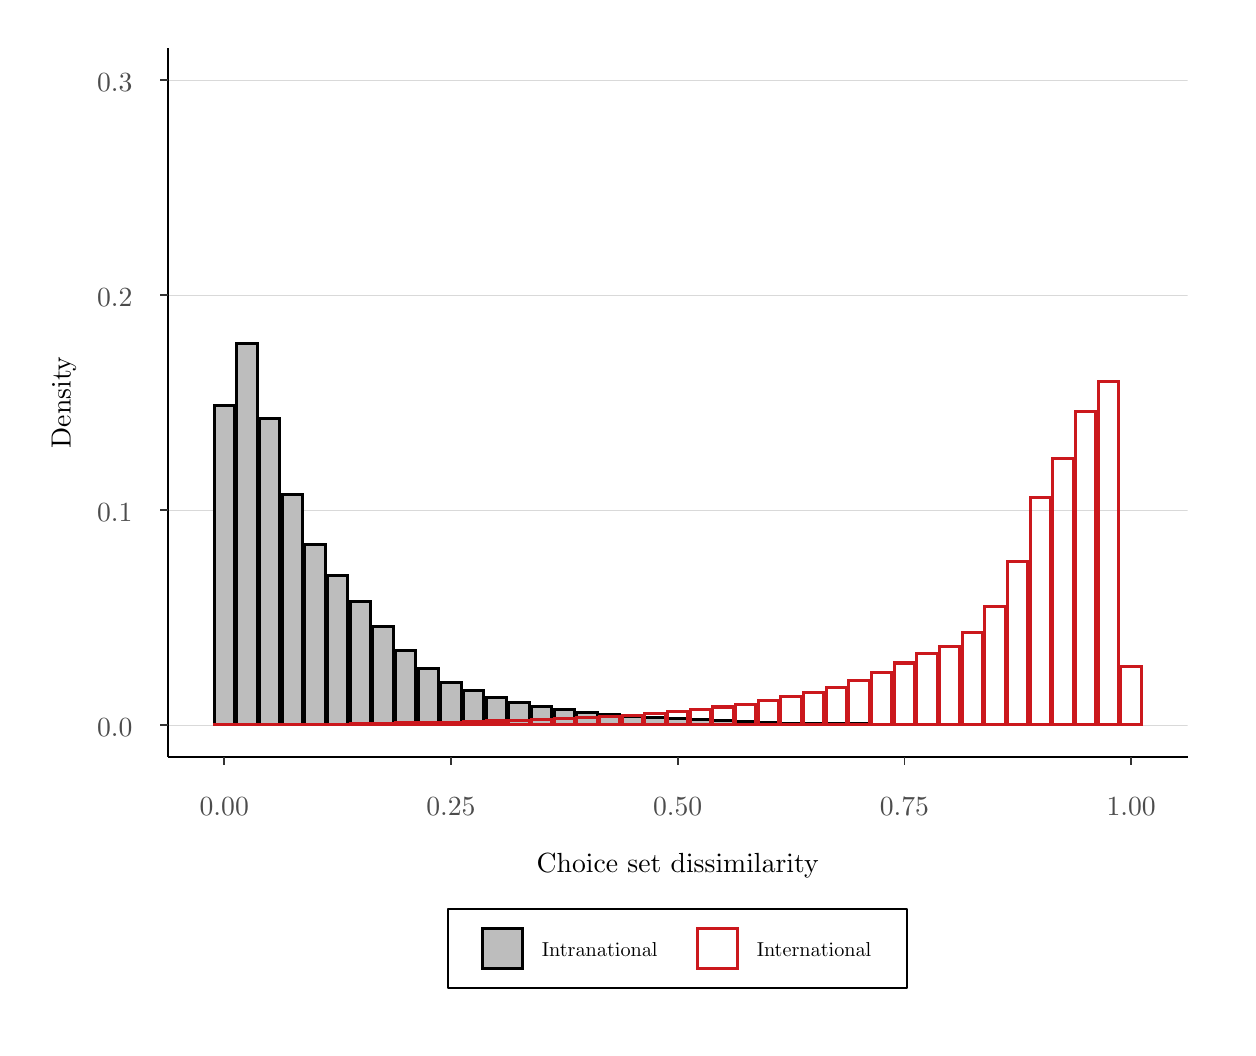
\begin{tikzpicture}[x=1pt,y=1pt]
\definecolor{fillColor}{RGB}{255,255,255}
\path[use as bounding box,fill=fillColor,fill opacity=0.00] (0,0) rectangle (433.62,361.35);
\begin{scope}
\path[clip] (  0.00,  0.00) rectangle (433.62,361.35);
\definecolor{drawColor}{RGB}{255,255,255}
\definecolor{fillColor}{RGB}{255,255,255}

\path[draw=drawColor,line width= 0.6pt,line join=round,line cap=round,fill=fillColor] (  0.00,  0.00) rectangle (433.62,361.35);
\end{scope}
\begin{scope}
\path[clip] ( 50.59, 97.75) rectangle (419.17,354.12);
\definecolor{drawColor}{RGB}{255,255,255}

\path[draw=drawColor,line width= 0.3pt,line join=round] ( 50.59,148.25) --
	(419.17,148.25);

\path[draw=drawColor,line width= 0.3pt,line join=round] ( 50.59,225.94) --
	(419.17,225.94);

\path[draw=drawColor,line width= 0.3pt,line join=round] ( 50.59,303.62) --
	(419.17,303.62);

\path[draw=drawColor,line width= 0.3pt,line join=round] (111.99, 97.75) --
	(111.99,354.12);

\path[draw=drawColor,line width= 0.3pt,line join=round] (193.92, 97.75) --
	(193.92,354.12);

\path[draw=drawColor,line width= 0.3pt,line join=round] (275.84, 97.75) --
	(275.84,354.12);

\path[draw=drawColor,line width= 0.3pt,line join=round] (357.76, 97.75) --
	(357.76,354.12);
\definecolor{drawColor}{gray}{0.85}

\path[draw=drawColor,line width= 0.1pt,line join=round] ( 50.59,109.40) --
	(419.17,109.40);

\path[draw=drawColor,line width= 0.1pt,line join=round] ( 50.59,187.09) --
	(419.17,187.09);

\path[draw=drawColor,line width= 0.1pt,line join=round] ( 50.59,264.78) --
	(419.17,264.78);

\path[draw=drawColor,line width= 0.1pt,line join=round] ( 50.59,342.47) --
	(419.17,342.47);
\definecolor{drawColor}{RGB}{0,0,0}
\definecolor{fillColor}{gray}{0.74}

\path[draw=drawColor,line width= 1.1pt,line cap=rect,fill=fillColor] ( 67.34,109.40) rectangle ( 74.72,224.75);
\definecolor{drawColor}{RGB}{203,24,29}

\path[draw=drawColor,line width= 1.1pt,line cap=rect] ( 67.34,109.40) rectangle ( 74.72,109.41);
\definecolor{drawColor}{RGB}{0,0,0}

\path[draw=drawColor,line width= 1.1pt,line cap=rect,fill=fillColor] ( 75.54,109.40) rectangle ( 82.91,247.28);
\definecolor{drawColor}{RGB}{203,24,29}

\path[draw=drawColor,line width= 1.1pt,line cap=rect] ( 75.54,109.40) rectangle ( 82.91,109.48);
\definecolor{drawColor}{RGB}{0,0,0}

\path[draw=drawColor,line width= 1.1pt,line cap=rect,fill=fillColor] ( 83.73,109.40) rectangle ( 91.10,220.14);
\definecolor{drawColor}{RGB}{203,24,29}

\path[draw=drawColor,line width= 1.1pt,line cap=rect] ( 83.73,109.40) rectangle ( 91.10,109.52);
\definecolor{drawColor}{RGB}{0,0,0}

\path[draw=drawColor,line width= 1.1pt,line cap=rect,fill=fillColor] ( 91.92,109.40) rectangle ( 99.29,192.63);
\definecolor{drawColor}{RGB}{203,24,29}

\path[draw=drawColor,line width= 1.1pt,line cap=rect] ( 91.92,109.40) rectangle ( 99.29,109.58);
\definecolor{drawColor}{RGB}{0,0,0}

\path[draw=drawColor,line width= 1.1pt,line cap=rect,fill=fillColor] (100.11,109.40) rectangle (107.49,174.64);
\definecolor{drawColor}{RGB}{203,24,29}

\path[draw=drawColor,line width= 1.1pt,line cap=rect] (100.11,109.40) rectangle (107.49,109.63);
\definecolor{drawColor}{RGB}{0,0,0}

\path[draw=drawColor,line width= 1.1pt,line cap=rect,fill=fillColor] (108.31,109.40) rectangle (115.68,163.34);
\definecolor{drawColor}{RGB}{203,24,29}

\path[draw=drawColor,line width= 1.1pt,line cap=rect] (108.31,109.40) rectangle (115.68,109.71);
\definecolor{drawColor}{RGB}{0,0,0}

\path[draw=drawColor,line width= 1.1pt,line cap=rect,fill=fillColor] (116.50,109.40) rectangle (123.87,153.97);
\definecolor{drawColor}{RGB}{203,24,29}

\path[draw=drawColor,line width= 1.1pt,line cap=rect] (116.50,109.40) rectangle (123.87,109.83);
\definecolor{drawColor}{RGB}{0,0,0}

\path[draw=drawColor,line width= 1.1pt,line cap=rect,fill=fillColor] (124.69,109.40) rectangle (132.06,144.86);
\definecolor{drawColor}{RGB}{203,24,29}

\path[draw=drawColor,line width= 1.1pt,line cap=rect] (124.69,109.40) rectangle (132.06,109.92);
\definecolor{drawColor}{RGB}{0,0,0}

\path[draw=drawColor,line width= 1.1pt,line cap=rect,fill=fillColor] (132.88,109.40) rectangle (140.26,136.40);
\definecolor{drawColor}{RGB}{203,24,29}

\path[draw=drawColor,line width= 1.1pt,line cap=rect] (132.88,109.40) rectangle (140.26,110.09);
\definecolor{drawColor}{RGB}{0,0,0}

\path[draw=drawColor,line width= 1.1pt,line cap=rect,fill=fillColor] (141.08,109.40) rectangle (148.45,129.74);
\definecolor{drawColor}{RGB}{203,24,29}

\path[draw=drawColor,line width= 1.1pt,line cap=rect] (141.08,109.40) rectangle (148.45,110.27);
\definecolor{drawColor}{RGB}{0,0,0}

\path[draw=drawColor,line width= 1.1pt,line cap=rect,fill=fillColor] (149.27,109.40) rectangle (156.64,124.84);
\definecolor{drawColor}{RGB}{203,24,29}

\path[draw=drawColor,line width= 1.1pt,line cap=rect] (149.27,109.40) rectangle (156.64,110.44);
\definecolor{drawColor}{RGB}{0,0,0}

\path[draw=drawColor,line width= 1.1pt,line cap=rect,fill=fillColor] (157.46,109.40) rectangle (164.83,121.85);
\definecolor{drawColor}{RGB}{203,24,29}

\path[draw=drawColor,line width= 1.1pt,line cap=rect] (157.46,109.40) rectangle (164.83,110.65);
\definecolor{drawColor}{RGB}{0,0,0}

\path[draw=drawColor,line width= 1.1pt,line cap=rect,fill=fillColor] (165.65,109.40) rectangle (173.03,119.47);
\definecolor{drawColor}{RGB}{203,24,29}

\path[draw=drawColor,line width= 1.1pt,line cap=rect] (165.65,109.40) rectangle (173.03,110.81);
\definecolor{drawColor}{RGB}{0,0,0}

\path[draw=drawColor,line width= 1.1pt,line cap=rect,fill=fillColor] (173.85,109.40) rectangle (181.22,117.54);
\definecolor{drawColor}{RGB}{203,24,29}

\path[draw=drawColor,line width= 1.1pt,line cap=rect] (173.85,109.40) rectangle (181.22,111.01);
\definecolor{drawColor}{RGB}{0,0,0}

\path[draw=drawColor,line width= 1.1pt,line cap=rect,fill=fillColor] (182.04,109.40) rectangle (189.41,116.15);
\definecolor{drawColor}{RGB}{203,24,29}

\path[draw=drawColor,line width= 1.1pt,line cap=rect] (182.04,109.40) rectangle (189.41,111.24);
\definecolor{drawColor}{RGB}{0,0,0}

\path[draw=drawColor,line width= 1.1pt,line cap=rect,fill=fillColor] (190.23,109.40) rectangle (197.60,114.95);
\definecolor{drawColor}{RGB}{203,24,29}

\path[draw=drawColor,line width= 1.1pt,line cap=rect] (190.23,109.40) rectangle (197.60,111.56);
\definecolor{drawColor}{RGB}{0,0,0}

\path[draw=drawColor,line width= 1.1pt,line cap=rect,fill=fillColor] (198.42,109.40) rectangle (205.80,113.82);
\definecolor{drawColor}{RGB}{203,24,29}

\path[draw=drawColor,line width= 1.1pt,line cap=rect] (198.42,109.40) rectangle (205.80,111.93);
\definecolor{drawColor}{RGB}{0,0,0}

\path[draw=drawColor,line width= 1.1pt,line cap=rect,fill=fillColor] (206.61,109.40) rectangle (213.99,113.03);
\definecolor{drawColor}{RGB}{203,24,29}

\path[draw=drawColor,line width= 1.1pt,line cap=rect] (206.61,109.40) rectangle (213.99,112.33);
\definecolor{drawColor}{RGB}{0,0,0}

\path[draw=drawColor,line width= 1.1pt,line cap=rect,fill=fillColor] (214.81,109.40) rectangle (222.18,112.46);
\definecolor{drawColor}{RGB}{203,24,29}

\path[draw=drawColor,line width= 1.1pt,line cap=rect] (214.81,109.40) rectangle (222.18,112.79);
\definecolor{drawColor}{RGB}{0,0,0}

\path[draw=drawColor,line width= 1.1pt,line cap=rect,fill=fillColor] (223.00,109.40) rectangle (230.37,112.09);
\definecolor{drawColor}{RGB}{203,24,29}

\path[draw=drawColor,line width= 1.1pt,line cap=rect] (223.00,109.40) rectangle (230.37,113.39);
\definecolor{drawColor}{RGB}{0,0,0}

\path[draw=drawColor,line width= 1.1pt,line cap=rect,fill=fillColor] (231.19,109.40) rectangle (238.56,111.76);
\definecolor{drawColor}{RGB}{203,24,29}

\path[draw=drawColor,line width= 1.1pt,line cap=rect] (231.19,109.40) rectangle (238.56,114.13);
\definecolor{drawColor}{RGB}{0,0,0}

\path[draw=drawColor,line width= 1.1pt,line cap=rect,fill=fillColor] (239.38,109.40) rectangle (246.76,111.45);
\definecolor{drawColor}{RGB}{203,24,29}

\path[draw=drawColor,line width= 1.1pt,line cap=rect] (239.38,109.40) rectangle (246.76,114.89);
\definecolor{drawColor}{RGB}{0,0,0}

\path[draw=drawColor,line width= 1.1pt,line cap=rect,fill=fillColor] (247.58,109.40) rectangle (254.95,111.06);
\definecolor{drawColor}{RGB}{203,24,29}

\path[draw=drawColor,line width= 1.1pt,line cap=rect] (247.58,109.40) rectangle (254.95,115.87);
\definecolor{drawColor}{RGB}{0,0,0}

\path[draw=drawColor,line width= 1.1pt,line cap=rect,fill=fillColor] (255.77,109.40) rectangle (263.14,110.71);
\definecolor{drawColor}{RGB}{203,24,29}

\path[draw=drawColor,line width= 1.1pt,line cap=rect] (255.77,109.40) rectangle (263.14,116.89);
\definecolor{drawColor}{RGB}{0,0,0}

\path[draw=drawColor,line width= 1.1pt,line cap=rect,fill=fillColor] (263.96,109.40) rectangle (271.33,110.30);
\definecolor{drawColor}{RGB}{203,24,29}

\path[draw=drawColor,line width= 1.1pt,line cap=rect] (263.96,109.40) rectangle (271.33,118.10);
\definecolor{drawColor}{RGB}{0,0,0}

\path[draw=drawColor,line width= 1.1pt,line cap=rect,fill=fillColor] (272.15,109.40) rectangle (279.53,110.02);
\definecolor{drawColor}{RGB}{203,24,29}

\path[draw=drawColor,line width= 1.1pt,line cap=rect] (272.15,109.40) rectangle (279.53,119.55);
\definecolor{drawColor}{RGB}{0,0,0}

\path[draw=drawColor,line width= 1.1pt,line cap=rect,fill=fillColor] (280.35,109.40) rectangle (287.72,109.84);
\definecolor{drawColor}{RGB}{203,24,29}

\path[draw=drawColor,line width= 1.1pt,line cap=rect] (280.35,109.40) rectangle (287.72,121.07);
\definecolor{drawColor}{RGB}{0,0,0}

\path[draw=drawColor,line width= 1.1pt,line cap=rect,fill=fillColor] (288.54,109.40) rectangle (295.91,109.77);
\definecolor{drawColor}{RGB}{203,24,29}

\path[draw=drawColor,line width= 1.1pt,line cap=rect] (288.54,109.40) rectangle (295.91,122.96);
\definecolor{drawColor}{RGB}{0,0,0}

\path[draw=drawColor,line width= 1.1pt,line cap=rect,fill=fillColor] (296.73,109.40) rectangle (304.10,109.74);
\definecolor{drawColor}{RGB}{203,24,29}

\path[draw=drawColor,line width= 1.1pt,line cap=rect] (296.73,109.40) rectangle (304.10,125.38);
\definecolor{drawColor}{RGB}{0,0,0}

\path[draw=drawColor,line width= 1.1pt,line cap=rect,fill=fillColor] (304.92,109.40) rectangle (312.30,109.67);
\definecolor{drawColor}{RGB}{203,24,29}

\path[draw=drawColor,line width= 1.1pt,line cap=rect] (304.92,109.40) rectangle (312.30,128.24);
\definecolor{drawColor}{RGB}{0,0,0}

\path[draw=drawColor,line width= 1.1pt,line cap=rect,fill=fillColor] (313.12,109.40) rectangle (320.49,109.60);
\definecolor{drawColor}{RGB}{203,24,29}

\path[draw=drawColor,line width= 1.1pt,line cap=rect] (313.12,109.40) rectangle (320.49,131.77);
\definecolor{drawColor}{RGB}{0,0,0}

\path[draw=drawColor,line width= 1.1pt,line cap=rect,fill=fillColor] (321.31,109.40) rectangle (328.68,109.53);
\definecolor{drawColor}{RGB}{203,24,29}

\path[draw=drawColor,line width= 1.1pt,line cap=rect] (321.31,109.40) rectangle (328.68,135.07);
\definecolor{drawColor}{RGB}{0,0,0}

\path[draw=drawColor,line width= 1.1pt,line cap=rect,fill=fillColor] (329.50,109.40) rectangle (336.87,109.49);
\definecolor{drawColor}{RGB}{203,24,29}

\path[draw=drawColor,line width= 1.1pt,line cap=rect] (329.50,109.40) rectangle (336.87,137.80);
\definecolor{drawColor}{RGB}{0,0,0}

\path[draw=drawColor,line width= 1.1pt,line cap=rect,fill=fillColor] (337.69,109.40) rectangle (345.07,109.47);
\definecolor{drawColor}{RGB}{203,24,29}

\path[draw=drawColor,line width= 1.1pt,line cap=rect] (337.69,109.40) rectangle (345.07,142.70);
\definecolor{drawColor}{RGB}{0,0,0}

\path[draw=drawColor,line width= 1.1pt,line cap=rect,fill=fillColor] (345.89,109.40) rectangle (353.26,109.49);
\definecolor{drawColor}{RGB}{203,24,29}

\path[draw=drawColor,line width= 1.1pt,line cap=rect] (345.89,109.40) rectangle (353.26,152.13);
\definecolor{drawColor}{RGB}{0,0,0}

\path[draw=drawColor,line width= 1.1pt,line cap=rect,fill=fillColor] (354.08,109.40) rectangle (361.45,109.47);
\definecolor{drawColor}{RGB}{203,24,29}

\path[draw=drawColor,line width= 1.1pt,line cap=rect] (354.08,109.40) rectangle (361.45,168.54);
\definecolor{drawColor}{RGB}{0,0,0}

\path[draw=drawColor,line width= 1.1pt,line cap=rect,fill=fillColor] (362.27,109.40) rectangle (369.64,109.44);
\definecolor{drawColor}{RGB}{203,24,29}

\path[draw=drawColor,line width= 1.1pt,line cap=rect] (362.27,109.40) rectangle (369.64,191.48);
\definecolor{drawColor}{RGB}{0,0,0}

\path[draw=drawColor,line width= 1.1pt,line cap=rect,fill=fillColor] (370.46,109.40) rectangle (377.84,109.42);
\definecolor{drawColor}{RGB}{203,24,29}

\path[draw=drawColor,line width= 1.1pt,line cap=rect] (370.46,109.40) rectangle (377.84,205.67);
\definecolor{drawColor}{RGB}{0,0,0}

\path[draw=drawColor,line width= 1.1pt,line cap=rect,fill=fillColor] (378.65,109.40) rectangle (386.03,109.41);
\definecolor{drawColor}{RGB}{203,24,29}

\path[draw=drawColor,line width= 1.1pt,line cap=rect] (378.65,109.40) rectangle (386.03,222.62);

\path[draw=drawColor,line width= 1.1pt,line cap=rect] (386.85,109.40) rectangle (394.22,233.49);

\path[draw=drawColor,line width= 1.1pt,line cap=rect] (395.04,109.40) rectangle (402.41,130.40);
\end{scope}
\begin{scope}
\path[clip] (  0.00,  0.00) rectangle (433.62,361.35);
\definecolor{drawColor}{RGB}{0,0,0}

\path[draw=drawColor,line width= 0.6pt,line join=round] ( 50.59, 97.75) --
	( 50.59,354.12);
\end{scope}
\begin{scope}
\path[clip] (  0.00,  0.00) rectangle (433.62,361.35);
\definecolor{drawColor}{gray}{0.30}

\node[text=drawColor,anchor=base east,inner sep=0pt, outer sep=0pt, scale=  1.00] at ( 37.84,105.27) {0.0};

\node[text=drawColor,anchor=base east,inner sep=0pt, outer sep=0pt, scale=  1.00] at ( 37.84,182.96) {0.1};

\node[text=drawColor,anchor=base east,inner sep=0pt, outer sep=0pt, scale=  1.00] at ( 37.84,260.65) {0.2};

\node[text=drawColor,anchor=base east,inner sep=0pt, outer sep=0pt, scale=  1.00] at ( 37.84,338.34) {0.3};
\end{scope}
\begin{scope}
\path[clip] (  0.00,  0.00) rectangle (433.62,361.35);
\definecolor{drawColor}{gray}{0.20}

\path[draw=drawColor,line width= 0.6pt,line join=round] ( 47.84,109.40) --
	( 50.59,109.40);

\path[draw=drawColor,line width= 0.6pt,line join=round] ( 47.84,187.09) --
	( 50.59,187.09);

\path[draw=drawColor,line width= 0.6pt,line join=round] ( 47.84,264.78) --
	( 50.59,264.78);

\path[draw=drawColor,line width= 0.6pt,line join=round] ( 47.84,342.47) --
	( 50.59,342.47);
\end{scope}
\begin{scope}
\path[clip] (  0.00,  0.00) rectangle (433.62,361.35);
\definecolor{drawColor}{RGB}{0,0,0}

\path[draw=drawColor,line width= 0.6pt,line join=round] ( 50.59, 97.75) --
	(419.17, 97.75);
\end{scope}
\begin{scope}
\path[clip] (  0.00,  0.00) rectangle (433.62,361.35);
\definecolor{drawColor}{gray}{0.20}

\path[draw=drawColor,line width= 0.6pt,line join=round] ( 71.03, 95.00) --
	( 71.03, 97.75);

\path[draw=drawColor,line width= 0.6pt,line join=round] (152.95, 95.00) --
	(152.95, 97.75);

\path[draw=drawColor,line width= 0.6pt,line join=round] (234.88, 95.00) --
	(234.88, 97.75);

\path[draw=drawColor,line width= 0.6pt,line join=round] (316.80, 95.00) --
	(316.80, 97.75);

\path[draw=drawColor,line width= 0.6pt,line join=round] (398.73, 95.00) --
	(398.73, 97.75);
\end{scope}
\begin{scope}
\path[clip] (  0.00,  0.00) rectangle (433.62,361.35);
\definecolor{drawColor}{gray}{0.30}

\node[text=drawColor,anchor=base,inner sep=0pt, outer sep=0pt, scale=  1.00] at ( 71.03, 76.73) {0.00};

\node[text=drawColor,anchor=base,inner sep=0pt, outer sep=0pt, scale=  1.00] at (152.95, 76.73) {0.25};

\node[text=drawColor,anchor=base,inner sep=0pt, outer sep=0pt, scale=  1.00] at (234.88, 76.73) {0.50};

\node[text=drawColor,anchor=base,inner sep=0pt, outer sep=0pt, scale=  1.00] at (316.80, 76.73) {0.75};

\node[text=drawColor,anchor=base,inner sep=0pt, outer sep=0pt, scale=  1.00] at (398.73, 76.73) {1.00};
\end{scope}
\begin{scope}
\path[clip] (  0.00,  0.00) rectangle (433.62,361.35);
\definecolor{drawColor}{RGB}{0,0,0}

\node[text=drawColor,anchor=base,inner sep=0pt, outer sep=0pt, scale=  1.00] at (234.88, 56.13) {Choice set dissimilarity};
\end{scope}
\begin{scope}
\path[clip] (  0.00,  0.00) rectangle (433.62,361.35);
\definecolor{drawColor}{RGB}{0,0,0}

\node[text=drawColor,rotate= 90.00,anchor=base,inner sep=0pt, outer sep=0pt, scale=  1.00] at ( 15.49,225.94) {Density};
\end{scope}
\begin{scope}
\path[clip] (  0.00,  0.00) rectangle (433.62,361.35);
\definecolor{drawColor}{RGB}{0,0,0}
\definecolor{fillColor}{RGB}{255,255,255}

\path[draw=drawColor,line width= 0.6pt,line join=round,line cap=round,fill=fillColor] (151.97, 14.45) rectangle (317.79, 42.80);
\end{scope}
\begin{scope}
\path[clip] (  0.00,  0.00) rectangle (433.62,361.35);

\path[] (162.97, 19.95) rectangle (180.32, 37.30);
\end{scope}
\begin{scope}
\path[clip] (  0.00,  0.00) rectangle (433.62,361.35);
\definecolor{drawColor}{RGB}{0,0,0}
\definecolor{fillColor}{gray}{0.74}

\path[draw=drawColor,line width= 1.1pt,line cap=rect,fill=fillColor] (164.39, 21.38) rectangle (178.89, 35.88);
\end{scope}
\begin{scope}
\path[clip] (  0.00,  0.00) rectangle (433.62,361.35);

\path[] (240.62, 19.95) rectangle (257.96, 37.30);
\end{scope}
\begin{scope}
\path[clip] (  0.00,  0.00) rectangle (433.62,361.35);
\definecolor{drawColor}{RGB}{203,24,29}

\path[draw=drawColor,line width= 1.1pt,line cap=rect] (242.04, 21.38) rectangle (256.54, 35.88);
\end{scope}
\begin{scope}
\path[clip] (  0.00,  0.00) rectangle (433.62,361.35);
\definecolor{drawColor}{RGB}{0,0,0}

\node[text=drawColor,anchor=base west,inner sep=0pt, outer sep=0pt, scale=  0.73] at (185.82, 25.60) {Intranational};
\end{scope}
\begin{scope}
\path[clip] (  0.00,  0.00) rectangle (433.62,361.35);
\definecolor{drawColor}{RGB}{0,0,0}

\node[text=drawColor,anchor=base west,inner sep=0pt, outer sep=0pt, scale=  0.73] at (263.46, 25.60) {International};
\end{scope}
\end{tikzpicture}
}
     \end{subfigure} \\
     \begin{subfigure}[t]{.49\textwidth}
        \centering
        \caption{$N^{F,ll'}_{p,t}$}
        \label{fig: redform_firm_c}
        \scalebox{0.45}{% Created by tikzDevice version 0.12.3.1 on 2022-10-03 21:47:02
% !TEX encoding = UTF-8 Unicode
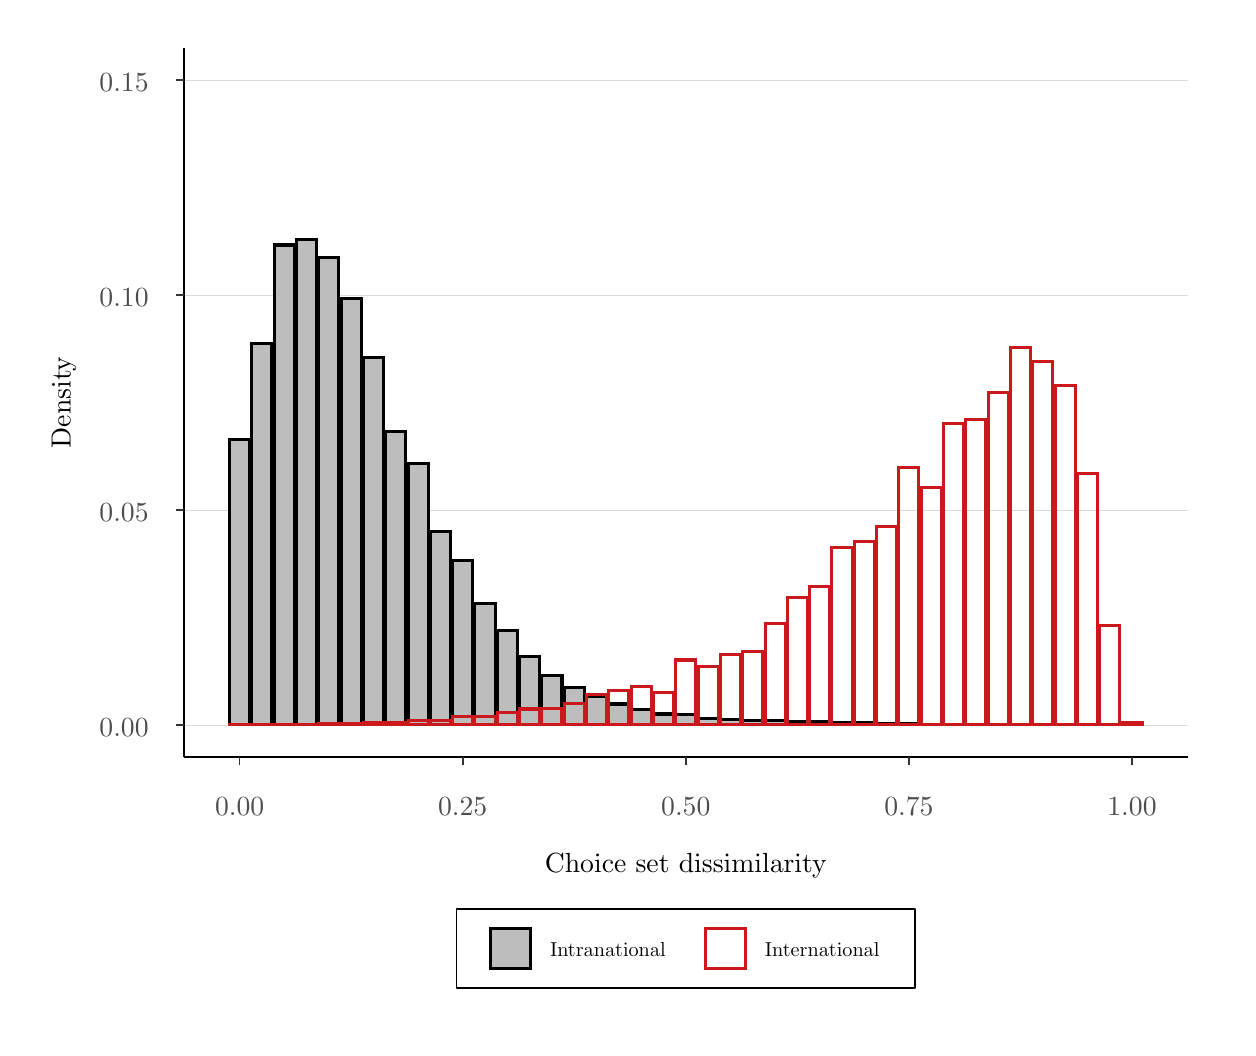
\begin{tikzpicture}[x=1pt,y=1pt]
\definecolor{fillColor}{RGB}{255,255,255}
\path[use as bounding box,fill=fillColor,fill opacity=0.00] (0,0) rectangle (433.62,361.35);
\begin{scope}
\path[clip] (  0.00,  0.00) rectangle (433.62,361.35);
\definecolor{drawColor}{RGB}{255,255,255}
\definecolor{fillColor}{RGB}{255,255,255}

\path[draw=drawColor,line width= 0.6pt,line join=round,line cap=round,fill=fillColor] ( -0.00,  0.00) rectangle (433.62,361.35);
\end{scope}
\begin{scope}
\path[clip] ( 56.47, 97.75) rectangle (419.17,354.12);
\definecolor{drawColor}{RGB}{255,255,255}

\path[draw=drawColor,line width= 0.3pt,line join=round] ( 56.47,148.25) --
	(419.17,148.25);

\path[draw=drawColor,line width= 0.3pt,line join=round] ( 56.47,225.94) --
	(419.17,225.94);

\path[draw=drawColor,line width= 0.3pt,line join=round] ( 56.47,303.62) --
	(419.17,303.62);

\path[draw=drawColor,line width= 0.3pt,line join=round] (116.89, 97.75) --
	(116.89,354.12);

\path[draw=drawColor,line width= 0.3pt,line join=round] (197.51, 97.75) --
	(197.51,354.12);

\path[draw=drawColor,line width= 0.3pt,line join=round] (278.12, 97.75) --
	(278.12,354.12);

\path[draw=drawColor,line width= 0.3pt,line join=round] (358.74, 97.75) --
	(358.74,354.12);
\definecolor{drawColor}{gray}{0.85}

\path[draw=drawColor,line width= 0.1pt,line join=round] ( 56.47,109.40) --
	(419.17,109.40);

\path[draw=drawColor,line width= 0.1pt,line join=round] ( 56.47,187.09) --
	(419.17,187.09);

\path[draw=drawColor,line width= 0.1pt,line join=round] ( 56.47,264.78) --
	(419.17,264.78);

\path[draw=drawColor,line width= 0.1pt,line join=round] ( 56.47,342.47) --
	(419.17,342.47);
\definecolor{drawColor}{RGB}{0,0,0}
\definecolor{fillColor}{gray}{0.74}

\path[draw=drawColor,line width= 1.1pt,line cap=rect,fill=fillColor] ( 72.95,109.40) rectangle ( 80.21,212.41);
\definecolor{drawColor}{RGB}{203,24,29}

\path[draw=drawColor,line width= 1.1pt,line cap=rect] ( 72.95,109.40) rectangle ( 80.21,109.61);
\definecolor{drawColor}{RGB}{0,0,0}

\path[draw=drawColor,line width= 1.1pt,line cap=rect,fill=fillColor] ( 81.01,109.40) rectangle ( 88.27,247.07);
\definecolor{drawColor}{RGB}{203,24,29}

\path[draw=drawColor,line width= 1.1pt,line cap=rect] ( 81.01,109.40) rectangle ( 88.27,109.44);
\definecolor{drawColor}{RGB}{0,0,0}

\path[draw=drawColor,line width= 1.1pt,line cap=rect,fill=fillColor] ( 89.08,109.40) rectangle ( 96.33,282.81);
\definecolor{drawColor}{RGB}{203,24,29}

\path[draw=drawColor,line width= 1.1pt,line cap=rect] ( 89.08,109.40) rectangle ( 96.33,109.49);
\definecolor{drawColor}{RGB}{0,0,0}

\path[draw=drawColor,line width= 1.1pt,line cap=rect,fill=fillColor] ( 97.14,109.40) rectangle (104.39,284.78);
\definecolor{drawColor}{RGB}{203,24,29}

\path[draw=drawColor,line width= 1.1pt,line cap=rect] ( 97.14,109.40) rectangle (104.39,109.65);
\definecolor{drawColor}{RGB}{0,0,0}

\path[draw=drawColor,line width= 1.1pt,line cap=rect,fill=fillColor] (105.20,109.40) rectangle (112.45,278.15);
\definecolor{drawColor}{RGB}{203,24,29}

\path[draw=drawColor,line width= 1.1pt,line cap=rect] (105.20,109.40) rectangle (112.45,109.75);
\definecolor{drawColor}{RGB}{0,0,0}

\path[draw=drawColor,line width= 1.1pt,line cap=rect,fill=fillColor] (113.26,109.40) rectangle (120.52,263.56);
\definecolor{drawColor}{RGB}{203,24,29}

\path[draw=drawColor,line width= 1.1pt,line cap=rect] (113.26,109.40) rectangle (120.52,109.95);
\definecolor{drawColor}{RGB}{0,0,0}

\path[draw=drawColor,line width= 1.1pt,line cap=rect,fill=fillColor] (121.32,109.40) rectangle (128.58,242.08);
\definecolor{drawColor}{RGB}{203,24,29}

\path[draw=drawColor,line width= 1.1pt,line cap=rect] (121.32,109.40) rectangle (128.58,110.14);
\definecolor{drawColor}{RGB}{0,0,0}

\path[draw=drawColor,line width= 1.1pt,line cap=rect,fill=fillColor] (129.38,109.40) rectangle (136.64,215.30);
\definecolor{drawColor}{RGB}{203,24,29}

\path[draw=drawColor,line width= 1.1pt,line cap=rect] (129.38,109.40) rectangle (136.64,110.32);
\definecolor{drawColor}{RGB}{0,0,0}

\path[draw=drawColor,line width= 1.1pt,line cap=rect,fill=fillColor] (137.45,109.40) rectangle (144.70,203.86);
\definecolor{drawColor}{RGB}{203,24,29}

\path[draw=drawColor,line width= 1.1pt,line cap=rect] (137.45,109.40) rectangle (144.70,111.14);
\definecolor{drawColor}{RGB}{0,0,0}

\path[draw=drawColor,line width= 1.1pt,line cap=rect,fill=fillColor] (145.51,109.40) rectangle (152.76,179.30);
\definecolor{drawColor}{RGB}{203,24,29}

\path[draw=drawColor,line width= 1.1pt,line cap=rect] (145.51,109.40) rectangle (152.76,110.97);
\definecolor{drawColor}{RGB}{0,0,0}

\path[draw=drawColor,line width= 1.1pt,line cap=rect,fill=fillColor] (153.57,109.40) rectangle (160.83,168.90);
\definecolor{drawColor}{RGB}{203,24,29}

\path[draw=drawColor,line width= 1.1pt,line cap=rect] (153.57,109.40) rectangle (160.83,112.55);
\definecolor{drawColor}{RGB}{0,0,0}

\path[draw=drawColor,line width= 1.1pt,line cap=rect,fill=fillColor] (161.63,109.40) rectangle (168.89,153.19);
\definecolor{drawColor}{RGB}{203,24,29}

\path[draw=drawColor,line width= 1.1pt,line cap=rect] (161.63,109.40) rectangle (168.89,112.51);
\definecolor{drawColor}{RGB}{0,0,0}

\path[draw=drawColor,line width= 1.1pt,line cap=rect,fill=fillColor] (169.69,109.40) rectangle (176.95,143.53);
\definecolor{drawColor}{RGB}{203,24,29}

\path[draw=drawColor,line width= 1.1pt,line cap=rect] (169.69,109.40) rectangle (176.95,113.98);
\definecolor{drawColor}{RGB}{0,0,0}

\path[draw=drawColor,line width= 1.1pt,line cap=rect,fill=fillColor] (177.76,109.40) rectangle (185.01,134.16);
\definecolor{drawColor}{RGB}{203,24,29}

\path[draw=drawColor,line width= 1.1pt,line cap=rect] (177.76,109.40) rectangle (185.01,115.15);
\definecolor{drawColor}{RGB}{0,0,0}

\path[draw=drawColor,line width= 1.1pt,line cap=rect,fill=fillColor] (185.82,109.40) rectangle (193.07,127.32);
\definecolor{drawColor}{RGB}{203,24,29}

\path[draw=drawColor,line width= 1.1pt,line cap=rect] (185.82,109.40) rectangle (193.07,115.32);
\definecolor{drawColor}{RGB}{0,0,0}

\path[draw=drawColor,line width= 1.1pt,line cap=rect,fill=fillColor] (193.88,109.40) rectangle (201.13,123.07);
\definecolor{drawColor}{RGB}{203,24,29}

\path[draw=drawColor,line width= 1.1pt,line cap=rect] (193.88,109.40) rectangle (201.13,117.26);
\definecolor{drawColor}{RGB}{0,0,0}

\path[draw=drawColor,line width= 1.1pt,line cap=rect,fill=fillColor] (201.94,109.40) rectangle (209.20,119.67);
\definecolor{drawColor}{RGB}{203,24,29}

\path[draw=drawColor,line width= 1.1pt,line cap=rect] (201.94,109.40) rectangle (209.20,120.43);
\definecolor{drawColor}{RGB}{0,0,0}

\path[draw=drawColor,line width= 1.1pt,line cap=rect,fill=fillColor] (210.00,109.40) rectangle (217.26,116.95);
\definecolor{drawColor}{RGB}{203,24,29}

\path[draw=drawColor,line width= 1.1pt,line cap=rect] (210.00,109.40) rectangle (217.26,121.75);
\definecolor{drawColor}{RGB}{0,0,0}

\path[draw=drawColor,line width= 1.1pt,line cap=rect,fill=fillColor] (218.06,109.40) rectangle (225.32,115.04);
\definecolor{drawColor}{RGB}{203,24,29}

\path[draw=drawColor,line width= 1.1pt,line cap=rect] (218.06,109.40) rectangle (225.32,123.14);
\definecolor{drawColor}{RGB}{0,0,0}

\path[draw=drawColor,line width= 1.1pt,line cap=rect,fill=fillColor] (226.13,109.40) rectangle (233.38,113.34);
\definecolor{drawColor}{RGB}{203,24,29}

\path[draw=drawColor,line width= 1.1pt,line cap=rect] (226.13,109.40) rectangle (233.38,121.24);
\definecolor{drawColor}{RGB}{0,0,0}

\path[draw=drawColor,line width= 1.1pt,line cap=rect,fill=fillColor] (234.19,109.40) rectangle (241.44,113.02);
\definecolor{drawColor}{RGB}{203,24,29}

\path[draw=drawColor,line width= 1.1pt,line cap=rect] (234.19,109.40) rectangle (241.44,132.86);
\definecolor{drawColor}{RGB}{0,0,0}

\path[draw=drawColor,line width= 1.1pt,line cap=rect,fill=fillColor] (242.25,109.40) rectangle (249.51,111.89);
\definecolor{drawColor}{RGB}{203,24,29}

\path[draw=drawColor,line width= 1.1pt,line cap=rect] (242.25,109.40) rectangle (249.51,130.44);
\definecolor{drawColor}{RGB}{0,0,0}

\path[draw=drawColor,line width= 1.1pt,line cap=rect,fill=fillColor] (250.31,109.40) rectangle (257.57,111.48);
\definecolor{drawColor}{RGB}{203,24,29}

\path[draw=drawColor,line width= 1.1pt,line cap=rect] (250.31,109.40) rectangle (257.57,134.96);
\definecolor{drawColor}{RGB}{0,0,0}

\path[draw=drawColor,line width= 1.1pt,line cap=rect,fill=fillColor] (258.37,109.40) rectangle (265.63,111.02);
\definecolor{drawColor}{RGB}{203,24,29}

\path[draw=drawColor,line width= 1.1pt,line cap=rect] (258.37,109.40) rectangle (265.63,135.92);
\definecolor{drawColor}{RGB}{0,0,0}

\path[draw=drawColor,line width= 1.1pt,line cap=rect,fill=fillColor] (266.44,109.40) rectangle (273.69,110.96);
\definecolor{drawColor}{RGB}{203,24,29}

\path[draw=drawColor,line width= 1.1pt,line cap=rect] (266.44,109.40) rectangle (273.69,146.09);
\definecolor{drawColor}{RGB}{0,0,0}

\path[draw=drawColor,line width= 1.1pt,line cap=rect,fill=fillColor] (274.50,109.40) rectangle (281.75,110.75);
\definecolor{drawColor}{RGB}{203,24,29}

\path[draw=drawColor,line width= 1.1pt,line cap=rect] (274.50,109.40) rectangle (281.75,155.61);
\definecolor{drawColor}{RGB}{0,0,0}

\path[draw=drawColor,line width= 1.1pt,line cap=rect,fill=fillColor] (282.56,109.40) rectangle (289.81,110.54);
\definecolor{drawColor}{RGB}{203,24,29}

\path[draw=drawColor,line width= 1.1pt,line cap=rect] (282.56,109.40) rectangle (289.81,159.45);
\definecolor{drawColor}{RGB}{0,0,0}

\path[draw=drawColor,line width= 1.1pt,line cap=rect,fill=fillColor] (290.62,109.40) rectangle (297.88,110.34);
\definecolor{drawColor}{RGB}{203,24,29}

\path[draw=drawColor,line width= 1.1pt,line cap=rect] (290.62,109.40) rectangle (297.88,173.57);
\definecolor{drawColor}{RGB}{0,0,0}

\path[draw=drawColor,line width= 1.1pt,line cap=rect,fill=fillColor] (298.68,109.40) rectangle (305.94,110.19);
\definecolor{drawColor}{RGB}{203,24,29}

\path[draw=drawColor,line width= 1.1pt,line cap=rect] (298.68,109.40) rectangle (305.94,175.65);
\definecolor{drawColor}{RGB}{0,0,0}

\path[draw=drawColor,line width= 1.1pt,line cap=rect,fill=fillColor] (306.74,109.40) rectangle (314.00,110.05);
\definecolor{drawColor}{RGB}{203,24,29}

\path[draw=drawColor,line width= 1.1pt,line cap=rect] (306.74,109.40) rectangle (314.00,181.01);
\definecolor{drawColor}{RGB}{0,0,0}

\path[draw=drawColor,line width= 1.1pt,line cap=rect,fill=fillColor] (314.81,109.40) rectangle (322.06,109.88);
\definecolor{drawColor}{RGB}{203,24,29}

\path[draw=drawColor,line width= 1.1pt,line cap=rect] (314.81,109.40) rectangle (322.06,202.38);
\definecolor{drawColor}{RGB}{0,0,0}

\path[draw=drawColor,line width= 1.1pt,line cap=rect,fill=fillColor] (322.87,109.40) rectangle (330.12,109.72);
\definecolor{drawColor}{RGB}{203,24,29}

\path[draw=drawColor,line width= 1.1pt,line cap=rect] (322.87,109.40) rectangle (330.12,195.21);
\definecolor{drawColor}{RGB}{0,0,0}

\path[draw=drawColor,line width= 1.1pt,line cap=rect,fill=fillColor] (330.93,109.40) rectangle (338.19,109.58);
\definecolor{drawColor}{RGB}{203,24,29}

\path[draw=drawColor,line width= 1.1pt,line cap=rect] (330.93,109.40) rectangle (338.19,218.47);
\definecolor{drawColor}{RGB}{0,0,0}

\path[draw=drawColor,line width= 1.1pt,line cap=rect,fill=fillColor] (338.99,109.40) rectangle (346.25,109.51);
\definecolor{drawColor}{RGB}{203,24,29}

\path[draw=drawColor,line width= 1.1pt,line cap=rect] (338.99,109.40) rectangle (346.25,219.61);
\definecolor{drawColor}{RGB}{0,0,0}

\path[draw=drawColor,line width= 1.1pt,line cap=rect,fill=fillColor] (347.05,109.40) rectangle (354.31,109.43);
\definecolor{drawColor}{RGB}{203,24,29}

\path[draw=drawColor,line width= 1.1pt,line cap=rect] (347.05,109.40) rectangle (354.31,229.64);
\definecolor{drawColor}{RGB}{0,0,0}

\path[draw=drawColor,line width= 1.1pt,line cap=rect,fill=fillColor] (355.12,109.40) rectangle (362.37,109.41);
\definecolor{drawColor}{RGB}{203,24,29}

\path[draw=drawColor,line width= 1.1pt,line cap=rect] (355.12,109.40) rectangle (362.37,245.76);
\definecolor{drawColor}{RGB}{0,0,0}

\path[draw=drawColor,line width= 1.1pt,line cap=rect,fill=fillColor] (363.18,109.40) rectangle (370.43,109.40);
\definecolor{drawColor}{RGB}{203,24,29}

\path[draw=drawColor,line width= 1.1pt,line cap=rect] (363.18,109.40) rectangle (370.43,240.77);

\path[draw=drawColor,line width= 1.1pt,line cap=rect] (371.24,109.40) rectangle (378.49,232.18);

\path[draw=drawColor,line width= 1.1pt,line cap=rect] (379.30,109.40) rectangle (386.56,200.40);

\path[draw=drawColor,line width= 1.1pt,line cap=rect] (387.36,109.40) rectangle (394.62,145.29);

\path[draw=drawColor,line width= 1.1pt,line cap=rect] (395.42,109.40) rectangle (402.68,110.18);
\end{scope}
\begin{scope}
\path[clip] (  0.00,  0.00) rectangle (433.62,361.35);
\definecolor{drawColor}{RGB}{0,0,0}

\path[draw=drawColor,line width= 0.6pt,line join=round] ( 56.47, 97.75) --
	( 56.47,354.12);
\end{scope}
\begin{scope}
\path[clip] (  0.00,  0.00) rectangle (433.62,361.35);
\definecolor{drawColor}{gray}{0.30}

\node[text=drawColor,anchor=base east,inner sep=0pt, outer sep=0pt, scale=  1.00] at ( 43.72,105.27) {0.00};

\node[text=drawColor,anchor=base east,inner sep=0pt, outer sep=0pt, scale=  1.00] at ( 43.72,182.96) {0.05};

\node[text=drawColor,anchor=base east,inner sep=0pt, outer sep=0pt, scale=  1.00] at ( 43.72,260.65) {0.10};

\node[text=drawColor,anchor=base east,inner sep=0pt, outer sep=0pt, scale=  1.00] at ( 43.72,338.34) {0.15};
\end{scope}
\begin{scope}
\path[clip] (  0.00,  0.00) rectangle (433.62,361.35);
\definecolor{drawColor}{gray}{0.20}

\path[draw=drawColor,line width= 0.6pt,line join=round] ( 53.72,109.40) --
	( 56.47,109.40);

\path[draw=drawColor,line width= 0.6pt,line join=round] ( 53.72,187.09) --
	( 56.47,187.09);

\path[draw=drawColor,line width= 0.6pt,line join=round] ( 53.72,264.78) --
	( 56.47,264.78);

\path[draw=drawColor,line width= 0.6pt,line join=round] ( 53.72,342.47) --
	( 56.47,342.47);
\end{scope}
\begin{scope}
\path[clip] (  0.00,  0.00) rectangle (433.62,361.35);
\definecolor{drawColor}{RGB}{0,0,0}

\path[draw=drawColor,line width= 0.6pt,line join=round] ( 56.47, 97.75) --
	(419.17, 97.75);
\end{scope}
\begin{scope}
\path[clip] (  0.00,  0.00) rectangle (433.62,361.35);
\definecolor{drawColor}{gray}{0.20}

\path[draw=drawColor,line width= 0.6pt,line join=round] ( 76.58, 95.00) --
	( 76.58, 97.75);

\path[draw=drawColor,line width= 0.6pt,line join=round] (157.20, 95.00) --
	(157.20, 97.75);

\path[draw=drawColor,line width= 0.6pt,line join=round] (237.82, 95.00) --
	(237.82, 97.75);

\path[draw=drawColor,line width= 0.6pt,line join=round] (318.43, 95.00) --
	(318.43, 97.75);

\path[draw=drawColor,line width= 0.6pt,line join=round] (399.05, 95.00) --
	(399.05, 97.75);
\end{scope}
\begin{scope}
\path[clip] (  0.00,  0.00) rectangle (433.62,361.35);
\definecolor{drawColor}{gray}{0.30}

\node[text=drawColor,anchor=base,inner sep=0pt, outer sep=0pt, scale=  1.00] at ( 76.58, 76.73) {0.00};

\node[text=drawColor,anchor=base,inner sep=0pt, outer sep=0pt, scale=  1.00] at (157.20, 76.73) {0.25};

\node[text=drawColor,anchor=base,inner sep=0pt, outer sep=0pt, scale=  1.00] at (237.82, 76.73) {0.50};

\node[text=drawColor,anchor=base,inner sep=0pt, outer sep=0pt, scale=  1.00] at (318.43, 76.73) {0.75};

\node[text=drawColor,anchor=base,inner sep=0pt, outer sep=0pt, scale=  1.00] at (399.05, 76.73) {1.00};
\end{scope}
\begin{scope}
\path[clip] (  0.00,  0.00) rectangle (433.62,361.35);
\definecolor{drawColor}{RGB}{0,0,0}

\node[text=drawColor,anchor=base,inner sep=0pt, outer sep=0pt, scale=  1.00] at (237.82, 56.13) {Choice set dissimilarity};
\end{scope}
\begin{scope}
\path[clip] (  0.00,  0.00) rectangle (433.62,361.35);
\definecolor{drawColor}{RGB}{0,0,0}

\node[text=drawColor,rotate= 90.00,anchor=base,inner sep=0pt, outer sep=0pt, scale=  1.00] at ( 15.49,225.94) {Density};
\end{scope}
\begin{scope}
\path[clip] (  0.00,  0.00) rectangle (433.62,361.35);
\definecolor{drawColor}{RGB}{0,0,0}
\definecolor{fillColor}{RGB}{255,255,255}

\path[draw=drawColor,line width= 0.6pt,line join=round,line cap=round,fill=fillColor] (154.91, 14.45) rectangle (320.72, 42.80);
\end{scope}
\begin{scope}
\path[clip] (  0.00,  0.00) rectangle (433.62,361.35);

\path[] (165.91, 19.95) rectangle (183.25, 37.30);
\end{scope}
\begin{scope}
\path[clip] (  0.00,  0.00) rectangle (433.62,361.35);
\definecolor{drawColor}{RGB}{0,0,0}
\definecolor{fillColor}{gray}{0.74}

\path[draw=drawColor,line width= 1.1pt,line cap=rect,fill=fillColor] (167.33, 21.38) rectangle (181.83, 35.88);
\end{scope}
\begin{scope}
\path[clip] (  0.00,  0.00) rectangle (433.62,361.35);

\path[] (243.56, 19.95) rectangle (260.90, 37.30);
\end{scope}
\begin{scope}
\path[clip] (  0.00,  0.00) rectangle (433.62,361.35);
\definecolor{drawColor}{RGB}{203,24,29}

\path[draw=drawColor,line width= 1.1pt,line cap=rect] (244.98, 21.38) rectangle (259.48, 35.88);
\end{scope}
\begin{scope}
\path[clip] (  0.00,  0.00) rectangle (433.62,361.35);
\definecolor{drawColor}{RGB}{0,0,0}

\node[text=drawColor,anchor=base west,inner sep=0pt, outer sep=0pt, scale=  0.73] at (188.75, 25.60) {Intranational};
\end{scope}
\begin{scope}
\path[clip] (  0.00,  0.00) rectangle (433.62,361.35);
\definecolor{drawColor}{RGB}{0,0,0}

\node[text=drawColor,anchor=base west,inner sep=0pt, outer sep=0pt, scale=  0.73] at (266.40, 25.60) {International};
\end{scope}
\end{tikzpicture}
}
    \end{subfigure}
    \begin{subfigure}[t]{.49\textwidth}
        \centering
        \caption{$\lambda^{F,ll'}_{p,t}$}
        \label{fig: redform_firm_e}
        \scalebox{0.45}{\input{figures/descriptives/P1_2_3_4_1_firm_n_s_na.tex}}
    \end{subfigure}
     \parbox{\textwidth}{
        \begin{spacing}{1} 
            {\footnotesize 
            \textit{Notes}: This figure plots the distribution for the count-based dissimilarity measures across NUTS2-region pairs. The unit of observation is at the product category-region $l$-region $l'$-year level. The grey bars plot the distribution for intranational pairs and the red bars do the same for international pairs. Panel (a) plots the count-based dissimilarity measure and panel (b) plots the expenditure-based dissimilarity measure for product varieties. Panel (c) and (d) do the same for firm-level dissimilarity measures. Note that panel (d) has two y-axes: the left y-axis scales with the different country region pairs and the right y-axis scales with the same country region pairs. }
        \end{spacing}}
\end{figure} 
To control for increased geographic differences across international region pairs, we re-estimate equation \ref{eq:border_effect_prices} for the four dissimilarity measures: 
\begin{linenomath*}
\begin{equation}\label{eq:border_effect_barcodes}
    y_{pll',t} = \beta B_{ll'} + \gamma d_{ll'} + \theta_l + \theta_{l'} +
                    \lambda_{p,t} + \varepsilon_{p(i)ll',t}
\end{equation}
\end{linenomath*}
where $y_{pll',t} = \left\{N^{B,ll'}_{p,t},\lambda^{B,ll'}_{p,t},N^{F,ll'}_{p,t},\lambda^{F,ll'}_{p,t}\right\}$. As before, we include a border dummy $B_{ll'}$ which is one when NUTS2-region $l$ and NUTS2-region $l'$ are an international region pair and zero otherwise, $d_{ll'}$, the log of the population-weighted distance between NUTS2-region $l$ and NUTS2-region $l'$ and product category-year $\lambda_{p,t}$ and region fixed effects $\theta_l$ and $\theta_{l'}$. 

Table \ref{tab: border_effects_choice} presents the baseline OLS estimates. First, columns (1), (4), (7) and (10) show that more distant regions are characterized by larger choice set differences independent of the dissimilarity measure used. Even if the distance coefficient considerably drops when conditioning on national borders in columns (2), (5), (7) and (11), it remains positive and significantly different from zero. For instance, column (2) shows that a 100\% increase in distance or a doubling of the distance between two regions increases choice set differences in terms of product variety counts by 5.1\%. Second, in line with Figures \ref{fig: redform_bar_c} and \ref{fig: redform_bar_e} we estimate large border effects for the product variety level dissimilarity measures. Within product category - years, column (2) illustrates that the overlap in choice sets decreases by more than 71.7ppt for international pairs. In other words, intranational pairs have more than five times as many product varieties in common compared to international pairs.\footnote{This number is obtained from the following calculation: $\frac{0.178+0.717}{0.178} = 5.028$} The border effect for expenditure-based choice set differences in column (5) is similarly estimated at 73.8ppt. Although there is cross-country heterogeneity in the average choice set dissimilarity for intranational pairs, columns (3) and (6) confirm that the border effects are positive, independent of the chosen baseline country. Third, the border effects for the dissimilarity measures at the firm level are lower relative to the ones at the product variety level. Column (8) shows that intranational pairs have more than five times as many firms in common compared to international pairs.\footnote{This number is obtained from the following calculation: $\frac{0.149+0.649}{0.149} = 5.35$} However, consistent with Figure \ref{fig: redform_firm_e} the firm-level border effects in terms of expenditure are substantially lower. Column (10) illustrates that consumers across international pairs spend on average more than 50\% on product varieties provided by firms common to both regions. Nevertheless, large differences remain as consumers in intranational pairs spend on average more than 97\% on product varieties provided by common firms. Columns (9) and (12) confirm that these results are robust to accounting for cross-country heterogeneity in differences for intranational pairs. \footnote{Throughout the analysis, Belgium seems to consistently have lower estimated border effects. The country dummy indicates that variation across Belgian region pairs is consistently higher compared to other countries. Therefore, the border effects from the Belgian perspective are lower.}

\begin{landscape}
    \begin{table}
        \centering
        \caption{Border effect: Choice set dissimilarity}
        \label{tab: border_effects_choice}
        \begin{spacing}{1.1}
            \scalebox{0.8}{
            \begin{tabular}{lcccccccccccc} \toprule
                & \multicolumn{3}{c}{$N^{B,ll'}_{p,t}$} & \multicolumn{3}{c}{$\lambda^{B,ll'}_{p,t}$}   
                & \multicolumn{3}{c}{$N^{F,ll'}_{p,t}$} & \multicolumn{3}{c}{$\lambda^{F,ll'}_{p,t}$} \\ 
                \cmidrule(lr){2-4} \cmidrule(lr){5-7} \cmidrule(lr){8-10} \cmidrule(lr){11-13}
                $y_{p(i)ll',t}$ & (1) & (2) & (3) & (4) & (5) & (6) & (7) & (8) & (9) & (10) & (11) & (12) \\ 
                \midrule
                $d_{ll'}$&$.426^{***}$&$.051^{***}$&$.058^{***}$&$.449^{***}$&$.062^{***}$&$.068^{***}$&$.376^{***}$&$.037^{***}$&$.048^{***}$&$.255^{***}$&$.035^{***}$&$.043^{***}$\\
&$(.009)$&$(.003)$&$(.002)$&$(.01)$&$(.003)$&$(.002)$&$(.008)$&$(.003)$&$(.002)$&$(.006)$&$(.003)$&$(.002)$\\
$B_{ll'}$&&$.717^{***}$&$.767^{***}$&&$.738^{***}$&$.778^{***}$&&$.649^{***}$&$.754^{***}$&&$.421^{***}$&$.474^{***}$\\
&&$(.003)$&$(.004)$&&$(.003)$&$(.004)$&&$(.004)$&$(.004)$&&$(.004)$&$(.004)$\\
$\mathbbm{1}\left(c(l) = c(l') = \text{BEL}\right)$&&&$.285^{***}$&&&$.251^{***}$&&&$.398^{***}$&&&$.362^{***}$\\
&&&$(.009)$&&&$(.009)$&&&$(.008)$&&&$(.008)$\\
$\mathbbm{1}\left(c(l) = c(l') = \text{FRA}\right)$&&&$.037^{***}$&&&$.002$&&&$.147^{***}$&&&$-.005^{*}$\\
&&&$(.007)$&&&$(.008)$&&&$(.008)$&&&$(.008)$\\
$\mathbbm{1}\left(c(l) = c(l') = \text{NLD}\right)$&&&$.138^{***}$&&&$.16^{***}$&&&$.256^{***}$&&&$.221^{***}$\\
&&&$(.007)$&&&$(.009)$&&&$(.007)$&&&$(.007)$\\
\midrule
$\theta_{l}$&$\checkmark$&$\checkmark$&$\checkmark$&$\checkmark$&$\checkmark$&$\checkmark$&$\checkmark$&$\checkmark$&$\checkmark$&$\checkmark$&$\checkmark$&$\checkmark$\\
$\theta_{l'}$&$\checkmark$&$\checkmark$&$\checkmark$&$\checkmark$&$\checkmark$&$\checkmark$&$\checkmark$&$\checkmark$&$\checkmark$&$\checkmark$&$\checkmark$&$\checkmark$\\
$\lambda_{c(i),t}$&$\checkmark$&$\checkmark$&$\checkmark$&$\checkmark$&$\checkmark$&$\checkmark$&$\checkmark$&$\checkmark$&$\checkmark$&$\checkmark$&$\checkmark$&$\checkmark$\\

$\hat{\mathbb{E}}\left(y_{c(i)ll',t}|\text{same}\right)$&.178&.178&.191&.117&.117&.129&.149&.149&.142&.023&.023&.025\\

$\beta - \gamma_{\text{BEL}}$&-&-&$.482^{***}$&-&-&$.526^{***}$&-&-&$.356^{***}$&-&-&$.112^{***}$\\
$\beta - \gamma_{\text{FRA}}$&-&-&$.73^{***}$&-&-&$.776^{***}$&-&-&$.607^{***}$&-&-&$.479^{***}$\\
$\beta - \gamma_{\text{NLD}}$&-&-&$.629^{***}$&-&-&$.617^{***}$&-&-&$.498^{***}$&-&-&$.253^{***}$\\

Nr. obs&4,627,670&4,627,670&4,627,670&4,627,670&4,627,670&4,627,670&4,627,670&4,627,670&4,627,670&4,627,670&4,627,670&4,627,670\\
$\text{Within R}^2$&0.51&0.94&0.94&0.50&0.91&0.92&0.47&0.88&0.90&0.35&0.64&0.66\\
\bottomrule

            \end{tabular}}
        \end{spacing}
        \parbox{1.2\textwidth}{
        \begin{spacing}{1} 
            {\footnotesize 
            \textit{Notes}: This table presents the OLS estimates from equation \label{eq:border_effect_barcodes}. Columns (1) - (3) and columns (4) - (6) estimate the results for the count-based and expenditure dissimilarity measure on the product variety level respectively. Columns (7) - (9) and columns (10) - (12) estimate the results for the count-based and expenditure dissimilarity measure on the firm level respectively. $\hat{\mathbb{E}}\left(y_{p(i)ll',t}|\text{same}\right)$ represents the average value of the left-hand side variable for the same country region pairs in all columns, expect in columns (3), (6), (9) and (12). In these columns, this number represents the average for the baseline country which is Germany. We cluster standard errors at the region pairs and present them in brackets below the coefficient estimates. Reported significance levels are at the $p<0.1^{*}$,$p<0.05^{**}$ and $p<0.01^{***}$ levels.} 
        \end{spacing}}
     \end{table}
\end{landscape}

In line with the results for the standard deviation of log price differences, there is much more heterogeneity across product categories compared to the time series. Figure \ref{fig: app_redform_choice_years} shows that the border effects are very stable for the count- and expenditure-based dissimilarity measures, independent of whether they are computed at the product variety or the firm level. In contrast, Figures \ref{fig: app_redform_choice_bar_cats_n} - \ref{fig: app_redform_choice_firm_cats_e} illustrate that, consistently across all the dissimilarity measures, there is substantial variation across product categories. For instance, Figure \ref{fig: app_redform_choice_firm_cats_e}, which plots the expenditure-based dissimilarity measure at the firm level, shows that choice set overlap varies from a little under 20ppt for deodorants to 60ppt for toilet paper all the while both product categories have a very similar choice set overlap for intranational pairs.

% Theoretical framework
\section{Theoretical Framework}\label{sec:theory}
The previous section showed that both LOP deviations and choice set differences are larger across international region pairs compared to intranational pairs. To jointly analyze both margins of geographic market segmentation, we now specify a flexible model of consumer preferences that provides a theoretically-grounded expression for regional cost-of-living differences. We use the structure of the model to decompose this expression into (1) LOP deviations, corrected for substitution effects, (2) pure taste differences and (3) choice set differences. 

\subsection{Consumer preferences}
As mentioned before, we model preferences as a nested CES utility system for three reasons. First, nested CES utility systems have shown the ability to fit empirical patterns in international economics while maintaining empirical tractability. In particular, \citet{Atkeson2008} and \citet{Hottman2016} show that nested CES system can rationalize the positive correlations between markups and firm size uncovered in \citet{Deloecker2012} and \citet{Deloecker2016} and between markup elasticities and firm size (see \citet{Berman2012, Amiti2019}). At the same, with data on prices and quantities, the elasticities of substitution are the only structural parameters one needs to estimate. Second, the nested CES utility system is part of a family of preference systems that admits an intuitive way to appraise the importance of taste differences for cost-of-living differences. \citet{Redding2020} show how, given a normalization of the average taste level across regions, the importance of taste differences can be uncovered by comparing cost-of-living differences obtained from the general nested CES price index to the Sato-Vartia CES price index, which restricts tastes to be equal across regions. Finally, CES systems are the workhorse model to understand differences in product variety in international trade (e.g. \citet{Feenstra1994,Broda2006}), urban economics (e.g. \citet{Handbury2015}) and macroeconomics (e.g. \citet{Romer1990,Jaravel2019}). To gauge the role of choice set differences, it intuitively depends on expenditure shares on the common set of product varieties and firms and estimates of the elasticities of substitution at each level of aggregation. 

\paragraph{Preferences}   Within each region consumers derive utility from a triple nested utility system. We assume that the final good aggregator is separable across the set of product categories $\mathcal{P}$, but we leave its particular functional form unspecified:
\begin{linenomath*}
    \begin{equation*}
        U(C_{l,t}) =  \mathit{F}_{l,t} \left(\left\{C_{pl,t}\right\}_{p = 1}^{\mathcal{P}}\right)
    \end{equation*}
\end{linenomath*}
\noindent where $\mathit{F}_{l,t}(\cdot)$ is the final good aggregator which can be region-specific and time-varying.\footnote{A Cobb-Douglas aggregator would satisfy this condition.} $C_{pl,t}$ is the real consumption level in region $l$ of product category $p$ at time $t$. Each product category-level consumption bundle $C_{pl,t}$ comprises two CES-utility nests that sequentially aggregate consumption of individual product varieties. In the middle nest, consumers allocate $C_{pl,t}$ across different firms that supply at least one product variety in that product category and region subject to the following aggregator: 
\begin{linenomath*}
    \begin{equation*}
        C_{pl,t} = \left(\sum_{f\in\mathcal{F}_{pl,t}}
                        \left(\phi_{fplt}C_{fpl,t}\right)^{\frac{\eta_p-1}{\eta_p}}
                    \right)^{\frac{\eta_p}{\eta_p-1}}
    \end{equation*} 
\end{linenomath*}
\noindent where $\mathcal{F}_{pl,t}$ is the set of firms that supply at least one product variety in product category $p$ in region $l$ at time $t$. $\phi_{fpl,t}$ represents consumer taste for product varieties supplied by firm $f$ in product category $p$ in region $l$ at time $t$ and $\eta_p$ denotes the constant elasticity of substitution across firms which is allowed to vary across product categories. In the lower nest, consumers allocate $C_{fpl,t}$ across product varieties, denoted by $i$ subject to another CES-utility aggregator: 
\begin{linenomath*}
    \begin{equation*}
        C_{il,t} = \left(\sum_{i\in\mathcal{B}_{fpl,t}}
                    \left(\phi_{il,t}C_{il,t}\right)^{\frac{\sigma_p-1}{\sigma_p}}
                  \right)^{\frac{\sigma_p}{\sigma_p-1}}
    \end{equation*} 
\end{linenomath*}
\noindent where $\mathcal{B}_{fpl,t}$ is the set of product varieties supplied by firm $f$ in product category $p$ in region $l$ at time $t$. $\phi_{il,t}$ captures consumer taste for product variety and $\sigma_p$ is the elasticity of substitution across product varieties which is also allowed to vary across product categories. $C_{il,t}$ is the corresponding consumption level of variety $i$ in region $l$ at time $t$.

\paragraph{Cost-of-living} Given the preference structure and the assumption that consumers maximize utility subject to their budget constraint $P_{l,t}C_{l,t} \leq I_{l,t}$, the product category-level cost-of-living for consumers in region $l$ at time $t$ is given by: 
\begin{linenomath*}
    \begin{equation*}
        P_{pl,t} = \left(\sum_{f\in\mathcal{F}_{pl,t}}
                        \left(\frac{P_{fpl,t}}{\phi_{fpl,t}}\right)^{1-\eta_p}\right)
                    ^{\frac{1}{1-\eta_p}}, \qquad \qquad \text{where} \qquad
        P_{fpl,t} = \left(\sum_{i\in\mathcal{B}_{fpl,t}}
                        \left(\frac{P_{il,t}}{\phi_{il,t}}\right)^{1-\sigma_p}\right)
                    ^{\frac{1}{1-\sigma_p}} 
    \end{equation*}
\end{linenomath*}
\noindent and where $P_{il,t}$ is the price of product variety $i$ in region $l$ at time $t$. 

%\subsection{Market Structure}
%We specify a parsimonious market structure in which we take the current set of firms and product varieties as given and in which firms set prices under Bertrand competition within countries and product categories. We choose this market structure for a couple of reasons. First, firms are allowed to be large relative to the market but they cannot affect the overall price level in the economy given the separable final good aggregator. Second, firms can have markups above one, but we abstract from retail markups which are subsumed in the marginal cost term. We do this because we want to stay close to the literature on international price differences which typically abstract from differences in retail markups (e.g. \citet{Verboven1996, Goldberg2001}) and because the international trade literature has often considered retail markups to be part of the distribution costs necessary to enter markets (\citet{Anderson2004}). Third, we assume that firms set prices at the country level. In this way, our market structure is in line with the mounting evidence that firms set prices uniformly across regions within countries (see \citet{Dellavigna2019}). Firms' profit maximization problem is given by: 
%\begin{linenomath*}
%    \begin{equation*}
%        \max_{P_{il,t}} \quad \Pi_{npl,t} = 
%            \sum_{l \in \mathcal{L}_n} \sum_{i \in \mathcal{B}_{fpl,t}} 
%            \left(P_{il,t} - MC_{il,t}\right)C_{il,t}
%    \end{equation*}
%\end{linenomath*}
%where $\mathcal{L}_n$ is the set of regions in country $n$, $P_{il,t}$ and $C_{il,t}$ are the unit price and quantity demanded of product variety $i$ in location $l$  and $MC_{il,t}$ is the marginal cost of providing product variety $i$ to region $l$, which we assume to be constant.\footnote{Assuming that marginal costs are constant is not without loss of generality. In this way, demand shocks in one region do not lead to price increases in other regions by affecting marginal costs. Nonetheless, assuming constant marginal costs is a common assumption to gain tractability over the spatial pricing problem with non-constant elasticities of substitution (e.g.\citet{Feenstra2020, Faber2021})}. This market structure gives rise to the following pricing rule (see Appendix XXX):
%\begin{linenomath*}
%    \begin{equation}\label{eq:pricing_rule}
%        P_{il,t} = \frac{\varepsilon_{fnp,t}}{\varepsilon_{fnp,t} - 1}MC_{il,t},
%        \qquad \text{where} \qquad
%        \varepsilon_{fnp,t} \equiv \eta_p - \left(\eta_p - 1 \right)S_{fpn,t} 
%    \end{equation}
%\end{linenomath*}
%The pricing rule for nested demand systems typically does not depend on the elasticity of substitution at the lowest nest. \citet{Hottman2016} illustrate that, within each firm nest, the firm is the monopoly supplier of the product varieties in that nest. Therefore, the profit maximization problem boils down to choosing the optimal firm-level price $P_{fpl,t}$ and to supplying the associated firm-level quantity at the lowest possible costs. Supplying at the lowest possible costs requires setting relative prices of the product varieties equal to their marginal costs. Consequently, markups do not vary across product varieties within the nests. Still, markups can differ across product categories, countries and time. Markups depend on the firm-level elasticity of substitution $\eta_p$ and the country-level market share $S_{fpn,t}$. Intuitively, higher firm-level elasticities of substitution reflect easier substitution across firms leading to lower markups. As the market share approaches zero,  firms have less and less influence on the product category level price, the elasticity of demand converges to the elasticity of substitution $\eta_p$ and markups are the same as under monopolistic competition. Conversely, as the market share grows the elasticity of demand falls and optimal markups increase. 
%
\subsection{Decomposing Cost-of-living Differences}
We decompose cost-of-living differences across two regions $l$ and $l'$ into three structural components: (1) LOP deviations, corrected for substitution effects (2) pure taste differences and (3) choice set differences. To this end, we define the share spent in region $l$ at time $t$ on firms that sell both in region $l$ and region $l'$ in product category $p$, $\lambda^{F,ll'}_{pl,t}$, and the share spent in region $l$ in at time $t$ on common product varieties sold by firm $f$ between region $l$ and region $l'$ in product category $p$, $\lambda^{B,ll'}_{fpl,t}$, as: 
\begin{linenomath*}
    \begin{equation*}
        \lambda^{F,ll'}_{pl,t} \equiv  
            \frac{\sum_{f \in \mathcal{F}^{ll'}_p}P_{fpl,t}C_{fpl,t}}
                 {\sum_{f \in \mathcal{F}_{pl,t}} P_{fpl,t}C_{fpl,t}}, \qquad 
        \lambda^{B,ll'}_{fpl,t} \equiv  
                 \frac{\sum_{i \in \mathcal{B}^{ll'}_{fp}}P_{il,t}C_{il,t}}
                      {\sum_{i \in \mathcal{B}_{fpl,t}} P_{il,t}C_{il,t}}
    \end{equation*}
\end{linenomath*}
\noindent where $\mathcal{F}^{ll'}_p$ is the set of firms that sell both to region $l$ and region $l'$ in product category $p$, $\mathcal{F}_{pl,t}$ is the set of all firms selling to region $l$ in product category $p$ at time $t$. Likewise, $\mathcal{B}^{ll'}_{fp}$ is the set of product varieties sold by firm $f$ that are available in region $l$ and region $l'$ in product category $p$ and $\mathcal{B}_{fpl,t}$ is the set of all product varieties that are available in region $l$ sold by firm $f$ in product category $p$ at time $t$. In addition, define for all firms and for all product varieties that sell in region $l$ and $l'$ in product category $p$ and the common market share in region $l$ at time $t$ as: 
\begin{linenomath*}
    \begin{equation*}
        S^{ll'}_{fpl,t} \equiv  
            \frac{P_{fpl,t}C_{fpl,t}}
                 {\sum_{f \in \mathcal{F}^{ll'}_{p}} P_{fpl,t}C_{fpl,t}}, \qquad 
        S^{ll'}_{il,t} \equiv  
                 \frac{P_{il,t}C_{il,t}}
                      {\sum_{i \in \mathcal{B}^{ll'}_{fp}} P_{il,t}C_{il,t}}
    \end{equation*}
\end{linenomath*}
\noindent This allows us to write the market shares of firms and product varieties that are available in region $l$ and region $l^{'}$ at time $t$ as a combination of their common market share and the share spent on common firms and product varieties in region $l$ at time $t$: 
\begin{linenomath*}
    \begin{equation*}
        S_{fpl,t} = S^{ll'}_{fpl,t} \lambda^{F,ll'}_{pl,t}
            \quad \forall f \in \mathcal{F}^{ll'}_{p}, \qquad \qquad 
        S_{il,t}  = S^{ll'}_{il,t} \lambda^{B,ll'}_{fpl,t}
            \quad \forall i \in \mathcal{B}^{ll'}_{fp}
    \end{equation*}
\end{linenomath*}

Using the definitions of the common market shares and the definitions of the expenditure shares on common firms and product varieties, we can write the difference in the cost-of-living between region $l'$ and $l$ for product category $p$ as the sum of two parts: 
\begin{linenomath*}
    \begin{equation*}
        \text{ln}\left(\frac{P_{pl',t}}{P_{pl,t}}\right)
            =   \frac{1}{N^{F,ll'}_{p}}
                \sum_{f \in \mathcal{F}^{ll'}_{p}} 
                \left[
                    \text{ln}\left(\frac{P_{fpl',t}}{P_{fpl,t}}\right)
                        -   \text{ln}\left(\frac{\varphi_{fpl',t}}{\varphi_{fpl,t}}\right)
                        +   \frac{1}{\eta_p-1}\text{ln}
                            \left(
                                \frac{S^{ll'}_{fpl',t}}{S^{ll'}_{fpl,t}}
                            \right)
                \right]
                + \frac{1}{\eta_p-1}
                    \text{ln}
                    \left(
                        \frac{\lambda^{F,ll'}_{pl',t}}{\lambda^{F,ll'}_{pl,t}}
                    \right)
    \end{equation*}
\end{linenomath*}
\noindent where $N^{F,ll'}_{p} \equiv |\mathcal{F}^{ll'}_{p}|$ is the number of firms in product category $p$ that sell to region $l'$ and $l$. The first part captures cost-of-living differences between the two regions that stem from price and expenditure differences within the set of firms that sell to both regions. This term intuitively depends on the differences in the unweighted geometric average price level across region $l^{'}$ and region $l$. This term is given by $\prod_{f \in \mathcal{F}^{ll'}_{p}} \left[P_{fpl',t}\bigg /P_{fpl,t}\right]^{\frac{1}{N^{F,ll'}_{p}}}$ and captures the fact that if firm-level prices are on average higher in region $l^{'}$, the cost-of-living in region $l^{'}$ should be higher.\footnote{This price index is also known as the Jevons price index.} However, to translate average price level differences into welfare-relevant numbers, two correction terms are required. The first is the difference in the unweighted geometric average taste levels across regions. Still, as in \citet{Redding2020}, we rule out cost-of-living differences that solely reflect differences in the average taste level across regions. The reason for this normalization is related to the fact we only observe choices and not the underlying utility levels. Hence, to avoid arbitrary shifts in cost-of-living levels, the cost-of-living levels should be the same across regions if prices and market shares are identical across regions. In practice, we make the following normalization: 
\begin{linenomath*}
    \begin{equation*}
    \tilde{\varphi}_{pl',t} \equiv 
        \prod_{f \in \mathcal{F}_{pl',t}} 
        \left[\varphi_{fpl,t} \right]^{\frac{1}{N^{ll'}_{p}}} 
    = 
        \prod_{f \in \mathcal{F}_{pl,t}} 
        \left[\varphi_{fpl,t} \right]^{\frac{1}{N^{ll'}_{p}}}
    \equiv  \tilde{\varphi}_{pl,t} 
\end{equation*}
\end{linenomath*}
\noindent Importantly, the normalization does not rule out taste differences across regions altogether. This is because the second correction term $\prod_{f \in \mathcal{F}^{ll'}_{p}} \left[\left(S^{ll'}_{fpl',t}\bigg / S^{ll'}_{fpl,t}\right)^{\frac{1}{\eta_p-1}}\right]^{\frac{1}{N^{F,ll'}_p}}$, which is the difference in the unweighted geometric average of the firm-level common market share across regions, represents a substitution effect and differences in consumer taste. The substitution effect captures the idea that in the presence of LOP deviations, consumers in different regions will have different expenditure shares as they substitute away from expensive bundles to bundles with lower relative prices. To reflect the relative importance of each product in total expenditure in each region, we need to correct the average price differences with a term that is a function of the market shares on common firms in each region.\footnote{Note that this is also the effect that gives rise to the traditionally-used Sato-Vartia weights. However, these weights are only the correct weights for CES preferences under the assumption that there are no differences in consumer taste: $\varphi_{fpl',t} = \varphi_{fpl,t} \quad \forall f \mathcal{F}^{ll'}_{p,t}$. The Sato-Vartia price index is, for instance, used by \citet{Handbury2015} to study cost-of-living differences across US cities.} To see why the second correction term also captures taste differences across regions, suppose that consumer tastes are more dispersed in region $l'$ relative to region $l$ and that there are no LOP deviations. Such a difference in dispersion in consumer taste leads consumers in $l^{'}$ to allocate a greater share of expenditure firms for which they have a high taste which results in a lower cost-of-living level for consumers in region $l^{'}$. As the greater dispersion in consumer taste also increases the dispersion in firm-level common market shares, it lowers the geometric average of common market shares reflecting the lower cost-of-living level. In addition to the difference in geometric average common market shares, the second correction term also depends on the firm-level elasticity of substitution. To see how, consider the limit when goods are perfect substitutes, $\eta_p \rightarrow\infty$. In this case, goods are perfect substitutes and common market shares are completely detached from taste-adjusted relative prices. Therefore, changes in taste-adjusted prices, originating from LOP deviations or taste differences, do not matter anymore for cost-of-living differences. In contrast, when firm-level bundles are very differentiated,  $\eta_p \rightarrow 1$, consumers value taste-adjusted price differences which translates into a much larger correction term given the same difference in the geometric average common market share.

The second term in the expression, $\left(\lambda^{F,ll'}_{pl',t}\bigg /\lambda^{F,ll'}_{pl,t}\right)^{\frac{1}{\eta_p-1}}$, accounts for choice set differences across regions. This term is the cross-sectional firm-level equivalent of the product variety term derived in \citet{Feenstra1994} and \citet{Broda2006} and depends on two moments of the data. For a given elasticity of substitution, the expenditure share on common firms in region $l^{'}$ region relative to region $l$ captures the relative importance of common firms in total expenditure. If the expenditure share on common firms is lower in region $l'$ it must mean that consumers in region $l^{'}$ have a better option outside of the set of common firms compared to consumers in region $l$ which translates into a lower cost of living in region $l^{'}$. The extent to which relative differences in expenditure on common firms lead to a lower cost of living depends on the firm-level elasticity of substitution. If this elasticity of substitution is high, bundles offered by firms are considered close substitutes. In this case, an increase in the choice set adds little additional substitution possibilities and the effect on the cost of living should be small.

The differences in the unweighted geometric average price level still depend on $P_{fpl,t}$ which are firm-level aggregators across product varieties part of the sets $\mathcal{B}_{fpl,t}$. To eliminate these firm-level price indices, we further decompose them like before:
\begin{linenomath*}
    \begin{equation}\label{eq:cle_decomp}
        \begin{aligned}
        \text{ln}\left(\frac{P_{pl',t}}{P_{pl,t}}\right)
            &=  \underbrace{
                    \frac{1}{N^{F,ll'}_{p}}
                    \sum_{f \in \mathcal{F}^{ll'}_{p}} 
                        \left[
                            \frac{1}{N^{B,ll'}_{p}}
                            \sum_{i \in \mathcal{B}^{ll'}_{p}} 
                            \text{ln}
                            \left(
                                \frac{P_{il',t}}{P_{il,t}}
                            \right)
                        \right]
                }_{\text{LOP deviations}} \\
                & \qquad + 
                \underbrace{
                    \frac{1}{N^{F,ll'}_{p}}
                    \sum_{f \in \mathcal{F}^{ll'}_{p}} 
                    \left[
                        \frac{1}{\eta_p-1}
                        \text{ln}
                        \left(
                            \frac{S^{ll'}_{fpl',t}}{S^{ll'}_{fpl,t}}
                        \right)
                        +
                        \frac{1}{\sigma_p-1}
                        \frac{1}{N^{B,ll'}_{p}}
                        \sum_{i \in \mathcal{B}^{ll'}_{p}} 
                            \text{ln}
                            \left(
                                \frac{S^{ll'}_{il',t}}{S^{ll'}_{il',t}}
                            \right)
                    \right]
                }_{\text{Common expenditure share differences}} \\
                & \qquad +
                \underbrace{
                    \frac{1}{\eta_p-1}
                    \text{ln}
                    \left(
                        \frac{\lambda^{ll'}_{pl',t}}{\lambda^{ll'}_{pl',t}}
                    \right)
                    + 
                    \frac{1}{\sigma_p-1}
                    \frac{1}{N^{F,ll'}_{p}}
                    \sum_{f \in \mathcal{F}^{ll'}_{p}} 
                        \text{ln}
                        \left(
                            \frac{\lambda^{ll'}_{fpl',t}}{\lambda^{ll'}_{fpl',t}}
                        \right)}_{\text{Choice set differences}}
    \end{aligned}
    \end{equation}
\end{linenomath*}
\noindent Equation \ref{eq:cle_decomp} illustrates that we can express cost-of-living differences across regions into three terms: (1) LOP deviations (2) common expenditure share differences and (3) choice set differences. Like before, we have normalized the unweighted geometric average of product variety-level taste differences such that cost-of-living levels are the same if prices, expenditure shares and choice sets are the same across regions: 
\begin{linenomath*}
    \begin{equation*}
        \tilde{\varphi}_{fpl',t} \equiv 
            \prod_{i \in \mathcal{B}_{fpl',t}} \left[\varphi_{il,t} \right]^{\frac{1}{N^{ll'}_{fp}}} 
        = 
            \prod_{i \in \mathcal{B}_{fpl,t}} \left[\varphi_{fpl,t} \right]^{\frac{1}{N^{ll'}_{fp}}}
        \equiv  \tilde{\varphi}_{fpl,t} 
    \end{equation*}
\end{linenomath*}

The common firm-level and product variety-level market share terms capture both substitution effects and taste differences. Isolating taste differences from LOP deviations, choice set differences and substitution effects is needed for the following reason. In a world without geographic market segmentation, LOP deviations and choice set differences only occur because the cost of physically moving goods to specific regions differs. Conversely, once the cost of physically moving goods is appropriately controlled for, LOP deviations and choice set differences should vanish. Importantly, also substitution effects zero in the absence of LOP deviations, but differences in taste differences remain. 

To isolate taste differences from the other terms, we follow \citet{Redding2020} and add and subtract: $\sum_{f \in \mathcal{F}^{ll'}_{p}} 
\omega_{fpl,t}
\left[
    \sum_{i \in \mathcal{B}^{ll'}_{p}} 
    \omega_{il,t}
    \text{ln}
    \left(
        \frac{P_{il',t}}{P_{il,t}}
    \right)
\right]$ from equation \ref{eq:cle_decomp}: 
\begin{linenomath*}
    \begin{equation}\label{eq:cle_decomp2}
        \begin{aligned}
        \text{ln}\left(\frac{P_{pl',t}}{P_{pl,t}}\right)
            &=  \underbrace{
                \sum_{f \in \mathcal{F}^{ll'}_{p}} 
                    \omega_{fpl,t}
                    \left[
                        \sum_{i \in \mathcal{B}^{ll'}_{p}} 
                        \omega_{il,t}
                        \text{ln}
                        \left(
                            \frac{P_{il',t}}{P_{il,t}}
                        \right)
                    \right]
                }_{\text{LOP deviations + Substitution Effect}} \\
                & \qquad + 
                \underbrace{
                    \frac{1}{N^{F,ll'}_{p}}
                    \sum_{f \in \mathcal{F}^{ll'}_{p}} 
                        \left[
                            \frac{1}{N^{B,ll'}_{p}}
                            \sum_{i \in \mathcal{B}^{ll'}_{p}} 
                            \left(
                                \frac{P_{il',t}}{P_{il,t}}
                            \right)
                        \right]
                    -
                    \sum_{f \in \mathcal{F}^{ll'}_{p}} 
                    \omega_{fpl,t}
                    \left[
                        \sum_{i \in \mathcal{B}^{ll'}_{p}} 
                        \omega_{il,t}
                        \text{ln}
                        \left(
                            \frac{P_{il',t}}{P_{il,t}}
                        \right)
                    \right]
                }_{\text{Taste differences}} \\
                & \qquad \qquad + 
                \underbrace{
                    \frac{1}{N^{F,ll'}_{p}}
                    \sum_{f \in \mathcal{F}^{ll'}_{p}} 
                    \left[
                        \frac{1}{\eta_p-1}
                        \text{ln}
                        \left(
                            \frac{S^{ll'}_{fpl',t}}{S^{ll'}_{fpl,t}}
                        \right)
                        +
                        \frac{1}{\sigma_p-1}
                        \frac{1}{N^{B,ll'}_{p}}
                        \sum_{i \in \mathcal{B}^{ll'}_{p}} 
                            \text{ln}
                            \left(
                                \frac{S^{ll'}_{il',t}}{S^{ll'}_{il',t}}
                            \right)
                    \right]
                }_{\text{Taste differences (ctd.)}} \\
                & \qquad +
                \underbrace{
                    \frac{1}{\eta_p-1}
                    \text{ln}
                    \left(
                        \frac{\lambda^{ll'}_{pl',t}}{\lambda^{ll'}_{pl',t}}
                    \right)
                    + 
                    \frac{1}{\sigma_p-1}
                    \frac{1}{N^{F,ll'}_{p}}
                    \sum_{f \in \mathcal{F}^{ll'}_{p}} 
                        \text{ln}
                        \left(
                            \frac{\lambda^{ll'}_{fpl',t}}{\lambda^{ll'}_{fpl',t}}
                        \right)}_{\text{Choice set differences}}
    \end{aligned}
    \end{equation}
\end{linenomath*}
where 
\begin{linenomath*}
    \begin{equation*}
        \omega_{fpl,t} 
            \equiv  \frac{
                        \frac{S^{ll'}_{fpl',t} - S^{ll'}_{fpl,t}}
                             {\text{ln }S^{ll'}_{fpl',t} - \text{ln }S^{ll'}_{fpl,t}}}
                         {\sum_{f \in \mathcal{F}^{ll'}_{p}} 
                            \frac{S^{ll'}_{fpl',t} - S^{ll'}_{fpl,t}}
                            {\text{ln }S^{ll'}_{fpl',t} - \text{ln }S^{ll'}_{fpl,t}}}, 
        \qquad 
        \omega_{il,t} 
            \equiv  \frac{
                        \frac{S^{ll'}_{il',t} - S^{ll'}_{il,t}}
                             {\text{ln }S^{ll'}_{il',t} - \text{ln }S^{ll'}_{il,t}}}
                         {\sum_{i \in \mathcal{B}^{ll'}_{fp}} 
                            \frac{S^{ll'}_{il',t} - S^{ll'}_{il,t}}
                            {\text{ln }S^{ll'}_{il',t} - \text{ln }S^{ll'}_{il,t}}}, 
    \end{equation*}
\end{linenomath*}
This expression decomposes cost-of-living differences into (1) LOP deviations, corrected for substitution effects, (2) pure taste differences and (3) choice set differences. The first part is the Sato-Vartia price index and captures only LOP deviations and substitution effects. The reason why it captures LOP deviations and substitution effects and not taste differences is that it is the ideal price index for common firms and product varieties for our nested CES preference system in the absence of taste differences.\footnote{This follows immediately from the derivation of the common market share terms when setting $\varphi_{fpl',t} = \varphi_{fpl,t} \quad \forall f \mathcal{F}^{ll'}_{p,t}$ and $\varphi_{il',t} = \varphi_{il,t} \quad \forall i \mathcal{B}^{ll'}_{fp,t}$} The second part captures pure taste differences. This is because this term is defined as the difference between the generalized price index, which allows for pure taste differences, and the Sato-Vartia price index, which abstracts from taste differences. This term is the cross-sectional analog to the taste-bias term derived in \citet{Redding2020}. The final part is the same as the one in equation \ref{eq:cle_decomp} and therefore still captures differences in choice sets between region $l'$ and $l$. This expression forms the basis to detect geographic market segmentation in section \ref{sec:border_effects_eu} and to separate taste differences from LOP deviations and choice set differences.

% Structural Estimation 
%%%%%%%%%%%%%%%%%%%%%%%%%%%%%%%%%%%%%%%%%%%%%%%%%%%%%%%%%%%%%%%%%%%%%%%%%%%%%%%%%%%%%%%%%%%%%%%%%%%%%%%%
%%%%%%%%%%%%%%%%%%%%%%%%%%%%%%%%%%%%%%%%%%%%%%%%%%%%%%%%%%%%%%%%%%%%%%%%%%%%%%%%%%%%%%%%%%%%%%%%%%%%%%%%
											   % Structural Estimation
%%%%%%%%%%%%%%%%%%%%%%%%%%%%%%%%%%%%%%%%%%%%%%%%%%%%%%%%%%%%%%%%%%%%%%%%%%%%%%%%%%%%%%%%%%%%%%%%%%%%%%%%
%%%%%%%%%%%%%%%%%%%%%%%%%%%%%%%%%%%%%%%%%%%%%%%%%%%%%%%%%%%%%%%%%%%%%%%%%%%%%%%%%%%%%%%%%%%%%%%%%%%%%%%%
\section{Structural Estimation}\label{sec:struc_est}
The expressions to compute the terms capturing taste and choice set differences crucially depend on the product variety- and firm-level elasticities of substitution. This section starts with estimating the product variety level elasticities of substitution and uses these estimates to construct firm-level price and quantity indices used to estimate the firm-level elasticities of substitution. In turn, we use these elasticities of substitution to construct cost-of-living differences and provide a first look into the size of cost-of-living differences and the importance of the three terms of the decomposition. 

\subsection{Elasticities of Substitution}
\subsubsection{Product variety-level elasticities - $\sigma_p$}
\paragraph{Estimation strategy}
To estimate the variety-level elasticity of substitution, we return to the product variety-level demand system. Demand for product variety $i$ in region $l$ at time $t$ is given by: 
\begin{linenomath*}
    \begin{equation*}
        C_{il,t} = \varphi_{il,t}^{\sigma_p-1}\left(\frac{P_{il,t}}{P_{fpl,t}}\right)^{-\sigma_p}C_{fpl,t}  
    \end{equation*}
\end{linenomath*}
\noindent as before $C_{il,t}$ is the consumed quantity in terms of metric units, $\varphi_{il,t}$ is the taste parameter and $P_{il,t}$ is the unit price for product variety $i$ in region $l$ at time $t$. In addition, $P_{fpl,t}$ and $C_{fpl,t}$ are the firm-level price index and consumption index in region $l$ at time $t$ and $\sigma_p$ is the product variety-level elasticity of substitution. Taking logs, we have: 
\begin{linenomath*}
    \begin{equation*}
        c_{il,t} = - \sigma_p p_{il,t} + \sigma_p p_{fpl,t} + c_{fpl,t} + (\sigma_p-1)\text{ln}\left(\varphi_{il,t}\right)
    \end{equation*} 
\end{linenomath*}
\noindent where small letters indicate logarithmic transformations of the level variables, e.g. $c_{il,t} \equiv \text{ln}\left(C_{il,t}\right)$. To estimate elasticities of substitution, we rely on the fact that after collapsing the household dimension in the transaction data the unit of observation is at the product variety-region-retail chain-time level. In practice, we consider the following model: 
\begin{linenomath*}
    \begin{equation}\label{eq:struc_est_elas_bar}
        c_{icl,t} = - \sigma_{p} p_{icl,t} + \theta_{icn(l),y(t)} + \theta_{icn(l),w(t)} + \lambda_{fpcl,t} + \varepsilon_{icl,t}
    \end{equation}
\end{linenomath*}
\noindent where $\varepsilon_{icl,t}$ subsumes the structural residual $\varphi_{il,t}$. Estimating the elasticities of substitution is subject to two endogeneity concerns. First, the price and consumption index $P_{fpl,t}$ and $C_{fpl,t}$ depend on the structural residuals that determine the quantity level. Second, if price variation is due to temporary discounts and promotions, product variety-level prices are likely correlated with the structural residual as well. We deal with the first issue by including firm-category-chain-NUTS2-time fixed effects $\lambda_{fpcl,t}$. The inclusion of a full set of fixed effects at the level of the indices is a common strategy to soak up this variation (e.g. \citet{Atkin2018, Fajgelbaum2020}). Moreover, the addition of $\lambda_{fpcl,t}$ also controls for any time-varying region-chain-specific demand shock that affects the product varieties of a specific firm in the same way. Collapsing the data at the variety-region-chain-time dimension is important to deal with the second identification concern. \citet{Dellavigna2019} illustrates that retail chains tend to follow uniform pricing strategies in which they frequently change prices over time through temporary discounts while limiting spatial variation to a minimum.\footnote{\citet{Dellavigna2019} point to managerial inertia, agency costs and threats to brand image as possible explanations for why retail chains adopt (potentially suboptimal) uniform pricing strategy.} The idea behind the identification strategy is that once we condition on the seasonal variation in prices and quantities, the lower-frequency variation in prices and quantities should reflect variation due to cost factors. To this end, we include highly-detailed product variety-chain-country-year fixed effects, $\theta_{icn(l),y(t)}$, and product variety-chain-country-week-of-the-year fixed effects, $\theta_{icn(l),w(t)}$. By interacting product variety-retail chain-country fixed effects with week-of-the-year and year effects, we capture seasonal variation in prices and quantities across variety-store cells at the weekly frequency and allow this pattern to shift across the years. However, even conditional on these fixed effects, there might still be price variation that is potentially correlated with occasional local demand shocks outside of this recurring seasonal pattern at the country level. Therefore, we instrument product variety-chain level prices with the average within-chain product variety level price across the other regions. The suitability of this \citet{Hausman1996}-type instrument relies on the exclusion restriction that chain-level pricing strategies are assumed not to be correlated anymore with local demand shocks after conditioning on the seasonal pattern of promotions and discounts.\footnote{In the estimation, we rely on the following moment condition $\mathbb{E}_{t}\left[{\varepsilon_{icl,t}|\bar{p}_{ic-l,t},\boldsymbol{\theta},\boldsymbol{\lambda}}\right] = 0$ and minimize the following GMM-objective function to obtain: 
\begin{equation*}
    \widehat{\sigma_p} = \argmin_{\sigma_p} \boldsymbol{M}(\sigma_p)'\boldsymbol{W}\boldsymbol{M}(\sigma_p) \qquad \forall p \in \mathcal{P} 
\end{equation*}
where 
\begin{equation*}
    M_{icl}(\sigma_p) = \mathbb{E}_{t}\left[\bar{p}_{ic-l,t}\varepsilon_{icl,t}(\sigma_p)\right], \qquad 
    \bar{p}_{ic-l,t} \equiv \frac{1}{N_{lc}} \sum_{k \in \mathcal{L}_c\setminus l} p_{ick,t}  
\end{equation*}
and $\boldsymbol{W}$ is a weighting matrix that weights the product variety-region moment conditions using the number of transactions associated with that product variety in that region. For this reason, our estimator is very similar to the one developed in \citet{Dellavigna2019} but different from \citet{Faber2021} which estimates brand-level elasticities in the US using only regional variation and no variation across retail chains and different from \citet{Atkin2018} which use it to estimate store-level elasticities in Mexico by collapsing the product variety dimension.}

\paragraph{Baseline results}    We estimate the elasticities using data at the product variety-retail chain-NUTS2-week level. We restrict the sample by placing restrictions on the frequency by which product varieties appear with positive sales. This is because there is widespread evidence of the existence of many zeros in scanner data which might potentially downwardly bias the elasticity estimates (e.g. \citet{Dube2021, Gandhi2022}). Given our broad focus on many product categories, it is hard to obtain exogenous variation in choice set determination for each product category as in \citet{Dube2021}. Instead, we choose to only include product varieties that are frequently purchased and thus suffer less from zero market shares. Below, we discuss the sensitivity of the estimates to alternative sample restrictions. Figure \ref{fig: app_elas_sigma_cats_weekly_50ptt} and Table \ref{tab: app_elas_sigma_cats_weekly} present the baseline OLS and IV estimates and report clustered standard errors at the product variety level. As expected, all OLS estimates have a negative sign and are precisely estimated but also represent quite inelastic residual demand curves. Their distribution is centered around $-1.02$ and has a 10\%-90\% spread of $[-1.96,-0.22]$. As the OLS estimates may still suffer from the simultaneous determination of prices and quantities, we instrument prices with the Hausman-type instrument. Figure \ref{fig: app_elas_sigma_cats_weekly_50ptt} shows that the IV-estimates are quite precisely estimated.\footnote{The precision of the IV-estimates is due to the generally high first-stage F-statistics. The Kleibergen-Paap statistic has an unreported 10\%-90\% range of $[12.35, 1098.44]$ across product categories.} In addition, they are almost always more negative compared to the OLS estimates. The IV estimates have a 10\%-90\% spread of $[-4.77,-1.15]$ with a median estimate of $-2.77$. While this product variety level estimates are more inelastic than the ones reported in \citet{Hottman2016}, the estimates are quantitatively in line with the estimates reported in different strands of literature. For instance, \citet{Dellavigna2019}, \citet{Faber2021} and \citet{Dopper2022} (for comparable US scanner data) and \citet{Fajgelbaum2020} (for US trade data at the product variety level) estimate very similar median estimates.\footnote{These papers report median elasticities of -2.6, -2.2, slightly below -2 and -2.53 respectively} In addition, we reject the null hypothesis that the elasticities are equal to the theoretical constraint of $-1$ for all but two product categories.\footnote{Unfortunately, we are unable to estimate elasticities of substitution for the Skincare - Makeup and Infant food categories because they have too few observations, conditional on the fixed effects. However, failing to obtain IV-estimates is common (see e.g. \citet{Hottman2016, Jaravel2019}) and we explain in section \ref{sec:border_effects_eu} how we deal with this to obtain the structural components.} Nevertheless, when estimating cost-of-living differences we experiment with more elastic elasticities of substitution that are closer to the ones from \citet{Hottman2016} and show that qualitative conclusions are robust.

\paragraph{Robustness}      We consider three different robustness checks. First, the baseline results are obtained by placing restrictions on how frequently positive sales are observed across weeks in a given year. Table \ref{tab: app_elas_sigma_cats_weekly} shows that the IV estimates are less elastic when we do not place any restrictions on the sample. In this case, the distribution of IV estimates has a 10\%-90\% range of $[-3.45,0.52]$. By placing ever stricter restrictions on the sample in terms of the frequency of positive sales and on the actual importance of different product varieties, the elasticity estimates become more elastic. When we restrict the frequency at 26 weeks and the product variety-level market share at 0.1\%, the distribution of elasticities is almost identical. Hence, we view the restriction on the frequency of more than or equal to 50\% as striking a good balance. Second, the baseline specification uses data at the weekly frequency. Figure \ref{fig: app_elas_sigma_cats_monthly_50ptt} and Table \ref{tab: app_elas_sigma_cats_monthly} shows the results when we estimate the elasticities using monthly data. The monthly IV estimates are almost always precisely estimated but they are also generally more inelastic. In addition, Table \ref{tab: app_elas_sigma_cats_monthly} indicates that there are slightly more product categories for which the theoretical constraint is not satisfied. For this reason, we stick with the weekly estimates as input for the subsequent analyses. Finally, the theoretical framework does not have a retail chain dimension and therefore there is some leeway as to how we deal with regional time-varying demand shocks. Table \ref{tab: app_elas_sigma_cats_weekly} provides an overview of the results when we experiment with alternative fixed effects. When we replace the firm-chain-category-region-time fixed effects with firm-chain-category-country-time fixed effects, we recover a more elastic median demand elasticity of $-3.89$, but also with a much wider range of $[-8.89;4.20]$.\footnote{One potential explanation for the more elastic demand estimates when including time-varying fixed effects at the country level is that if promotional activities come with temporary price reductions and if there is regional variation in promotional activity, only including time-varying fixed effects at the country level will overestimate the elasticity of demand. This is because in this case the increase in consumption and the fall in the price are both driven by the same promotion. As $\sigma_{c,prom} > 0$ and  $\sigma_{p,prom} < 0$ the elasticity of substitution would be downward biased.} In addition, the number of product categories where the theoretical restriction is not satisfied rises from 2 to 10. When we only include firm-category-region-time fixed effects instead of the firm-chain-category-region-time fixed effects, the 10\%-90\% range is $[-5.01,-1.15]$ centered around $-3.12$. This specification also leads to more estimates that violate the theoretical constraint. The robustness exercise of cost-of-living differences to alternative elasticities includes the implied elasticities with country-level fixed effects and the results presented below are also robust to using alternative fixed effects in the estimation of the elasticities.

\subsubsection{Firm-level elasticities - $\eta_p$}
\paragraph{Estimation strategy}     To estimate the firm-level elasticities of substitution, consider the residual demand curve for firm $f$ in product category $p$ in region $l$ at time $t$: 
\begin{linenomath*}
    \begin{equation*}
        C_{fpl,t} = \varphi_{pfl,t}^{\eta_p-1}\left(\frac{P_{fpl,t}}{P_{pl,t}}\right)^{-\eta_p}C_{pl,t}  
    \end{equation*}
\end{linenomath*}
\noindent where $C_{pfl,t}$ and  $P_{fpl,t}$ are the firm-level quantity and price level, $P_{pl,t}$ and $C_{pl,t}$ are the aggregate price and consumption index and $\eta_p$ governs how consumers substitute across firms in product category $p$. $\varphi_{pfl,t}$ is the firm-level taste parameter that shifts demand across all product varieties in product category $p$ offered by firm $f$. At any level of aggregation, the utility functions are homogeneous of degree 1 in the taste parameters. Therefore, without an additional normalization, it is impossible to distinguish between the firm-level tastes $\phi_{fpl,t}$ and the aggregated product-variety level taste parameters within each product category-firm-region-time combination. For this reason, we follow \cite{Hottman2016} and make two useful normalizations regarding the taste parameters: 
\begin{linenomath*}
    \begin{equation*}
        \tilde{\varphi}_{fpl,t} 
            \equiv  \left(\prod_{i \in \mathcal{B}_{fpl,t}} \varphi_{il,t} \right)^{\frac{1}{N_{fpl,t}}}
            =       \left(\prod_{f \in \mathcal{F}_{fpl,t+1}} \varphi_{fpl,t+1} \right)^{\frac{1}{N_{fpl,t+1}}}
            \equiv \tilde{\varphi}_{pl,t+1}
    \end{equation*}
\end{linenomath*}
\noindent where $N_{fpl,t}$ is the number of product varieties that firm $f$ sells in product category $p$ in region $l$ at time $t$ and $N_{pl,t}$ is the associated number of firms. We normalize the product variety level taste parameters $\varphi_{il,t}$ such that the geometric mean of the product variety level taste parameters within each product category-firm-region-time does not change over time.\footnote{Note that this normalization is without loss of generality as any geometric aggregator would be suitable (see \cite{Redding2020}). In addition, this normalization is different from the normalization we performed in the derivation of the cost-of-living differences across regions in two ways. First, the previous normalization was about ruling out that pure changes in tastes at the firm or product variety level across regions can induce changes in cost-of-living differences. In this case, the normalization is about how the product variety- en firm-level shifters are related within each region and is based on the fact that the utility aggregators are homogeneous of degree 1 in the taste parameters. Second, this normalization is about the full set of product varieties offered in region $l$. The previous normalization only covers the set of product varieties that is common across the two regions.} In this way, we ensure that differences in firm-level consumption levels conditional on relative prices and aggregate consumption are captured by $\varphi_{pfl,t}$ and any shifts in product variety-level consumption levels conditional on relative prices and firm-level consumption levels is captured by the $\varphi_{il,t}$'s. Consider the log transformation of the firm-level residual demand curve: 
\begin{linenomath*}
    \begin{equation*}
        c_{fpl,t} = - \eta_p p_{fpl,t} + \eta_p p_{pl,t} + c_{pl,t} + (\eta_p-1)\text{ln}\left(\varphi_{pfl,t}\right)
    \end{equation*} 
\end{linenomath*}

\noindent and its empirical counterpart are given by: 

\begin{linenomath*}
    \begin{equation}\label{eq:struc_est_elas_firm}
        c_{pfl,t} = - \eta_{p} p_{pfl,t} + \theta_{pfl} + \lambda_{pl,t} + \varepsilon_{pfl,t}
    \end{equation}
\end{linenomath*}
\noindent where $\varepsilon_{pfl,t}$ subsumes $\varphi_{pfl,t}$. We take the following steps to estimate equation \ref{eq:struc_est_elas_firm}. First, we obtain the firm-level consumption and price indices by aggregating product variety-level quantity and price using the baseline product-variety level elasticities of substitution and the backed-out product variety-level taste parameters.\footnote{We back out the product variety level demand shifters using: $$\varphi_{il,t} =  \frac{P_{il,t}}{\tilde{P}_{fpl,t}}\left(\frac{S_{il,t}}{\tilde{S}_{fpl,t}}\right)^{\frac{1}{\sigma_p-1}}\tilde{\varphi}_{fpl,t}$$ where $\tilde{P}_{fpl,t} \equiv \left(\prod_{i \in \mathcal{B}_{fpl,t}} P_{il,t}\right)^{\frac{1}{N_{fpl,t}}}$ and $\tilde{S}_{fpl,t} \equiv \left(\prod_{i \in \mathcal{B}_{fpl,t}} S_{il,t}\right)^{\frac{1}{N_{fpl,t}}}$.} We include two sets of fixed effects to deal with omitted variables and use an instrument to construct moment conditions. First, including the product category-region-time fixed effects $\lambda_{pl,t}$ captures variation stemming from the unobserved product category-level price and consumption indices, given by $p_{pl,t}$ and $c_{pl,t}$ respectively. In addition, these fixed effects pick up time-varying regional demand shocks that affect all firms similarly in product category $p$ in region $l$. Second, $\theta_{pfl}$ are category-firm-region fixed effects and pick up persistent differences in firm-level tastes across regions, such as the unweighted average product variety-level taste parameters $\varphi_{pfl,t}$. As the local demand shocks might still drive both consumption and prices, we rely on an instrument that follows from the structure of the demand system and the normalization imposed on the average product variety-level demand shifters. In particular, the firm-level price index can be written as a product of two intuitive terms (see Appendix \ref{app:theory_residuals_instrument} and \citet{Hottman2016}): 
\begin{linenomath*}
    \begin{equation*}
        P_{fpl,t} = \tilde{P}_{fpl,t} 
                    \left(
                        \sum_{i \in \mathcal{B}_{fpl,t}} \frac{S_{il,t}}{\tilde{S}_{fpl,t}} \tilde{\varphi}_{fpl,t}^{\sigma_p-1}
                    \right)^{\frac{1}{1-\sigma_p}}
    \end{equation*}
\end{linenomath*}
\noindent The first part is the unweighted geometric average across product variety-level prices offered by firm $f$ in product category $p$, region $l$ at time $t$. When firms simultaneously set the average firm-level price and taste parameter, this first part is correlated with the firm-level taste shifter $\varphi_{pfl,t}$. The second part of this expression depends on the dispersion in product variety level market shares within each product category-firm-region-time cell. Intuitively, more dispersion in market shares, reflecting greater dispersion in taste-adjusted prices, leads to a fall in the geometric average and thus an increase in the sum of market shares relative to their geometric average. However, as this sum is raised to a negative power ($1-\sigma_p$) greater dispersion within product category-firm-region-time cells leads to a fall in the firm-level price index. As the relative within product category-firm-region-time market shares do not depend on the firm-level taste shifter and the unweighted geometric average across product varieties is partialled out with the inclusion of $\theta_{pfl}$, the second part is uncorrelated with the firm-level taste parameter and therefore a suitable instrument.\footnote{This instrument relies on the presence of multi-product firms and imperfect substitutability across product varieties which. When only one product is supplied, the dispersion in market share is zero. If product varieties are perfect substitutes ($\sigma_p \rightarrow \infty$), market shares are disconnected from taste-adjusted prices leading to no dispersion in market shares. In the estimation, we rely on the following moment condition $\mathbb{E}_{t}\left[{\varepsilon_{fpl,t}|p^{D}_{fpl,t},\boldsymbol{\theta},\boldsymbol{\lambda}}\right] = 0$ and minimize the following GMM-objective function to obtain: 
\begin{equation*}
    \widehat{\eta_p} = \argmin_{\eta_p} \boldsymbol{M}(\eta_p)'\boldsymbol{W}\boldsymbol{M}(\eta_p) \qquad \forall p \in \mathcal{P} 
\end{equation*}
where 
\begin{equation*}
    M_{pfl}(\eta_p) = \mathbb{E}_{t}\left[p^{D}_{fpl,t}\varepsilon_{fpl,t}(\eta)\right], \qquad 
    p^{D}_{fpl,t} \equiv 
        \frac{1}{1-\hat{\sigma}_p}
        \text{ln}\left(\sum_{i \in \mathcal{B}_{fpl,t}}\frac{S_{il,t}}{\tilde{S}_{fpl,t}} \tilde{\varphi}_{fpl,t}^{\hat{\sigma_p}-1}\right)
\end{equation*}
and $\boldsymbol{W}$ is a weighting matrix that weights the product variety-region moment conditions using the number of transactions associated with that firm in that region.}

\paragraph{Baseline results}    We estimate the elasticities using data at the firm-NUTS2-week level and restrict the baseline sample to include all purchases on product varieties that register positive sales in more than 50\% of the time within a year. We present the baseline in Figure \ref{fig: app_elas_eta_cats_weekly_50ptt} and report an overview of all specifications in Table \ref{tab: app_elas_eta_cats_weekly_q} with clustered standard errors at the firm level. The OLS estimates are all negative, precisely estimated and almost always fall within the $[-2,-1]$ range. Given that firm-level prices conditional on the fixed effects might still be correlated with the structural residual, we turn to the IV estimates. First, the instruments are strong as the F-statistics of the first-stage regressions are almost always larger than the conventional rejection levels for weak instruments.\footnote{More precisely, the first-stage Kleibergergen-Paap F-statistics have a 10\%-90\% range of $[15.60;5,830.67]$ while the smallest F-statistics is $7.24$.} Second, the IV estimates imply more elastic residual demand curves as they are centered around $-3.10$ and have a 10\%-90\% range of $[-4.84,-1.71]$.\footnote{The range of firm-level elasticities is very close to the range of product-variety level elasticities. Given that we do not impose any restriction on their relative magnitude, this does not pose a problem for our analysis per se.} This range is still lower, but comparatively closer to the estimates in \citet{Hottman2016} which estimate firm-level elasticities between $[-7.3,-2.6]$ centered around $-3.9$. The estimation routine successfully ends for all product categories and we reject the null hypothesis that the elasticities are different from the theoretical constraint of $-1$ for all the product categories.

\paragraph{Robustness} We consider four robustness checks. First, Table \ref{tab: app_elas_eta_cats_weekly_q} shows that the elasticities are very similar across different sample restrictions. The reason for this is that the data becomes much less sparse when collapsing both retail chain and product variety dimensions such that imposing the same sample restrictions does not result in markedly different samples. At this level of aggregation, it does not matter whether we consider the full sample or the frequent sample. Second, similar to the product-variety estimates, the distribution of monthly firm-level elasticities is shifted upwards when we collapse the data at the monthly level. While the elasticities are still precisely estimated, Table \ref{tab: app_elas_eta_cats_monthly_q} shows that the distribution of monthly estimates is centered around $-1.66$ with a range $[-3.20,-1.32]$. Third, the baseline estimation includes product category-firm-region fixed effects and thus only controls for persistent differences across firms within regions. However, if retail chains and firms coordinate on seasonal price changes and promotion, a better identification strategy could be to use time variation conditional on seasonal shocks. For this reason, we re-estimate equation \ref{eq:struc_est_elas_firm} by replacing the $\theta_{pfl}$ fixed effects with product category-firm-region-yer fixed effects, $\theta_{pfl,y(t)}$, and product category-firm-region fixed effects-week-of-the-year $\theta_{pfl,w(t)}$. This set of fixed effects also flexibly controls for seasonal demand shocks that could drive both firm-level demand and prices. Nevertheless, Table \ref{tab: app_elas_eta_cats_weekly_q} shows that the distribution of elasticities is largely unaffected.

\paragraph{Cross-country Heterogeneity} The assumption that elasticities of substitution are common across countries is necessary to exactly decompose cost-of-living differences across regions. To check the validity of this assumption for the firm-level elasticities of substitution, we estimate country-level elasticities of substitution by interacting the price variable in equation \ref{eq:struc_est_elas_firm} with country dummies. Tables \ref{tab: app_elas_eta_cats_weekly_q_BE} - \ref{tab: app_elas_eta_cats_weekly_q_DE} present the elasticity of substitution estimates at the country level and Table \ref{tab: app_elas_eta_cats_weekly_q_comp} provides a comparison of the distribution of the IV-estimates across the different countries. Tables \ref{tab: app_elas_eta_cats_weekly_q_BE} - \ref{tab: app_elas_eta_cats_weekly_q_DE} confirm that the elasticities are still precisely estimated and satisfy the theoretical constraint in almost all cases. Even though there is some variation across countries for a couple of product categories, Table \ref{tab: app_elas_eta_cats_weekly_q_comp} shows that these differences do not imply large systematic differences in the country-level distributions. Therefore, the assumption of equal elasticities does not seem to be very restrictive.

\paragraph{Implied markups}    An additional check on the estimated elasticities of substitution is to see whether they imply firm-level markups when combined with an assumption on how firms set prices. If we assume that firms set prices in a simultaneous move Bertrand game, firm-level markups depend on the firm-level elasticity of substitution and on the firm-level market share in location $l$ at time $t$.\footnote{In particular, under Bertrand competition in prices, markups are given by: 
    \begin{equation}\label{eq:pricing_rule}
        P_{il,t} = \frac{\varepsilon_{fnp,t}}{\varepsilon_{fnp,t} - 1}MC_{il,t},
        \qquad \text{where} \qquad
        \varepsilon_{fnp,t} \equiv \eta_p - \left(\eta_p - 1 \right)S_{fpn,t} 
    \end{equation}} 
Figure \ref{fig: struct_est_markups} shows the full distribution of recovered firm-level markups across product category-firm-country-year observations. We recover a median firm-level markup of 1.5 which implies that the median firm charges a 50\% price premium over its marginal costs.

How sensible are these markup estimates? Because there is little empirical evidence on the level of firm-level markups for a comparable set of product categories in Europe, we benchmark our estimates to the broader literature on markup estimation. There are two broad strands in this literature. First, the demand approach estimates markups by specifying a model of demand and market structure. Markups are computed based on the estimated demand parameters and the optimal markup function as implied by the assumed market structure. Our approach falls in this strand. Other papers that take the demand approach to estimate markups for a broad set of product categories are \citet{Hottman2016} and \citet{Dopper2022}. While \citet{Hottman2016} finds a median markup of 1.31, \citet{Dopper2022} reports a median markup of 2.08.\footnote{These papers report different measures of the markup. \citet{Hottman2016} report a median $\frac{P-MC}{MC}$ of 0.31, which results in a median $\frac{P}{MC}$ of 1.31. \citet{Dopper2022} report a median Lerner index $\frac{P-MC}{P}$ of 0.48 which results in a median $\frac{P}{MC}$ of 2.08.} Second, \citet{Deloecker2012} pioneered the production approach in which the combination of cost minimization and an estimated output elasticity on a completely variable input in production yields markup estimates. \citet{Deloecker2016} and \citet{Deloecker2020} report a median elasticity of 1.6 for Indian manufacturing firms and an average markup of 1.6 for public US companies. Given that our estimates are close to estimates from both of these strands in the literature, we consider our markup estimates as sensible.  

\begin{figure}[H]
    \centering
    \caption{Firm-level markup distribution}
    \label{fig: struct_est_markups}
    % Created by tikzDevice version 0.12.3.1 on 2022-09-12 13:44:44
% !TEX encoding = UTF-8 Unicode
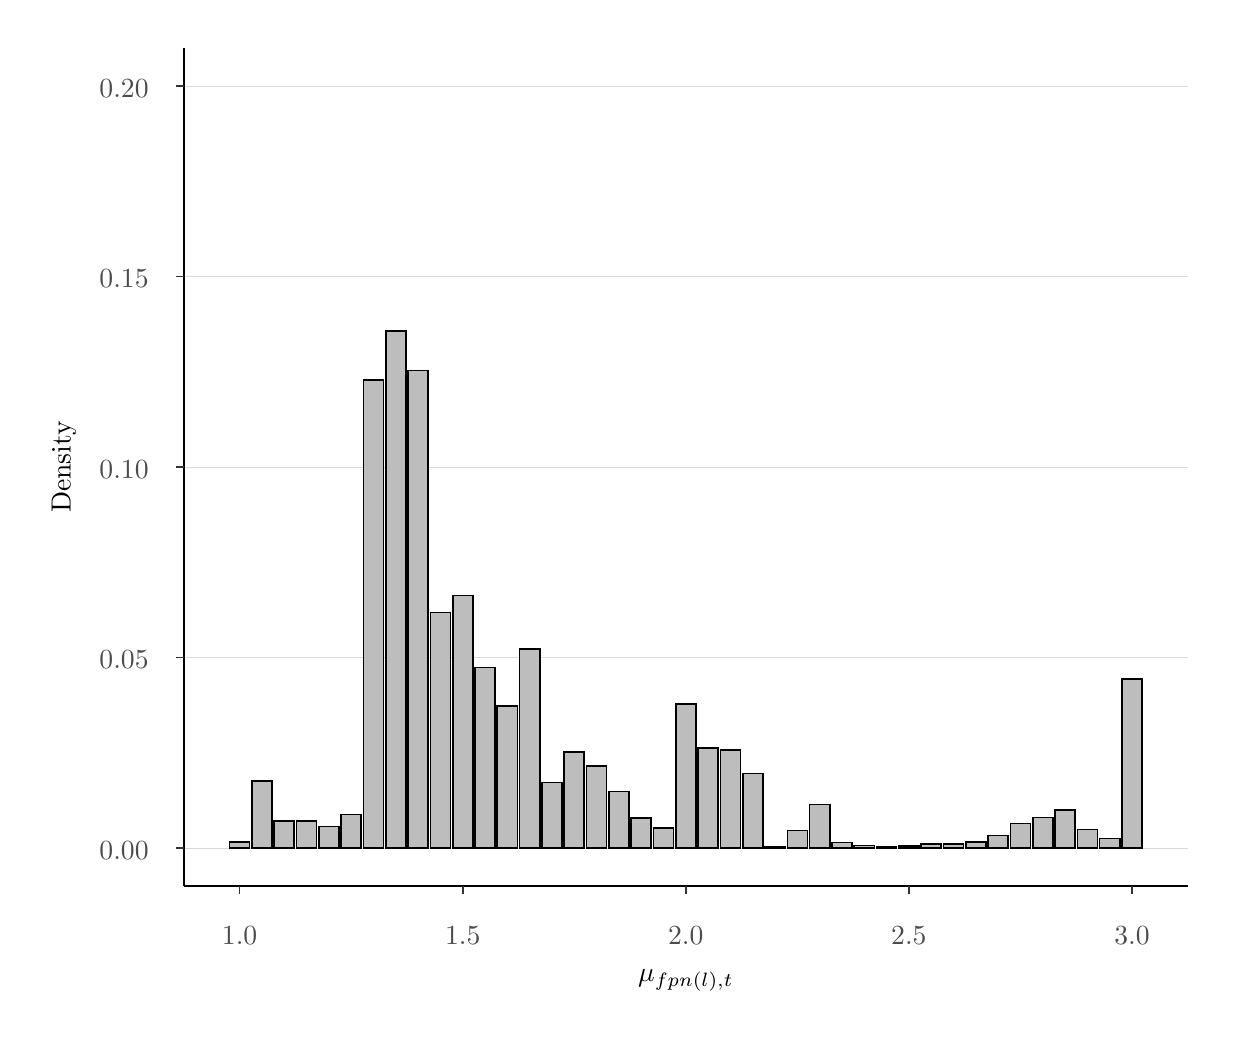
\begin{tikzpicture}[x=1pt,y=1pt]
\definecolor{fillColor}{RGB}{255,255,255}
\path[use as bounding box,fill=fillColor,fill opacity=0.00] (0,0) rectangle (433.62,361.35);
\begin{scope}
\path[clip] (  0.00,  0.00) rectangle (433.62,361.35);
\definecolor{drawColor}{RGB}{255,255,255}
\definecolor{fillColor}{RGB}{255,255,255}

\path[draw=drawColor,line width= 0.6pt,line join=round,line cap=round,fill=fillColor] ( -0.00,  0.00) rectangle (433.62,361.35);
\end{scope}
\begin{scope}
\path[clip] ( 56.47, 51.15) rectangle (419.17,354.12);
\definecolor{drawColor}{RGB}{255,255,255}

\path[draw=drawColor,line width= 0.3pt,line join=round] ( 56.47, 99.35) --
	(419.17, 99.35);

\path[draw=drawColor,line width= 0.3pt,line join=round] ( 56.47,168.21) --
	(419.17,168.21);

\path[draw=drawColor,line width= 0.3pt,line join=round] ( 56.47,237.07) --
	(419.17,237.07);

\path[draw=drawColor,line width= 0.3pt,line join=round] ( 56.47,305.92) --
	(419.17,305.92);

\path[draw=drawColor,line width= 0.3pt,line join=round] (116.89, 51.15) --
	(116.89,354.12);

\path[draw=drawColor,line width= 0.3pt,line join=round] (197.51, 51.15) --
	(197.51,354.12);

\path[draw=drawColor,line width= 0.3pt,line join=round] (278.12, 51.15) --
	(278.12,354.12);

\path[draw=drawColor,line width= 0.3pt,line join=round] (358.74, 51.15) --
	(358.74,354.12);
\definecolor{drawColor}{gray}{0.85}

\path[draw=drawColor,line width= 0.1pt,line join=round] ( 56.47, 64.92) --
	(419.17, 64.92);

\path[draw=drawColor,line width= 0.1pt,line join=round] ( 56.47,133.78) --
	(419.17,133.78);

\path[draw=drawColor,line width= 0.1pt,line join=round] ( 56.47,202.64) --
	(419.17,202.64);

\path[draw=drawColor,line width= 0.1pt,line join=round] ( 56.47,271.49) --
	(419.17,271.49);

\path[draw=drawColor,line width= 0.1pt,line join=round] ( 56.47,340.35) --
	(419.17,340.35);
\definecolor{drawColor}{RGB}{0,0,0}
\definecolor{fillColor}{gray}{0.74}

\path[draw=drawColor,line width= 0.6pt,line cap=rect,fill=fillColor] ( 72.95, 64.92) rectangle ( 80.21, 67.13);

\path[draw=drawColor,line width= 0.6pt,line cap=rect,fill=fillColor] ( 81.01, 64.92) rectangle ( 88.27, 89.09);

\path[draw=drawColor,line width= 0.6pt,line cap=rect,fill=fillColor] ( 89.08, 64.92) rectangle ( 96.33, 74.76);

\path[draw=drawColor,line width= 0.6pt,line cap=rect,fill=fillColor] ( 97.14, 64.92) rectangle (104.39, 74.76);

\path[draw=drawColor,line width= 0.6pt,line cap=rect,fill=fillColor] (105.20, 64.92) rectangle (112.45, 72.65);

\path[draw=drawColor,line width= 0.6pt,line cap=rect,fill=fillColor] (113.26, 64.92) rectangle (120.52, 77.04);

\path[draw=drawColor,line width= 0.6pt,line cap=rect,fill=fillColor] (121.32, 64.92) rectangle (128.58,234.00);

\path[draw=drawColor,line width= 0.6pt,line cap=rect,fill=fillColor] (129.38, 64.92) rectangle (136.64,251.84);

\path[draw=drawColor,line width= 0.6pt,line cap=rect,fill=fillColor] (137.45, 64.92) rectangle (144.70,237.44);

\path[draw=drawColor,line width= 0.6pt,line cap=rect,fill=fillColor] (145.51, 64.92) rectangle (152.76,149.99);

\path[draw=drawColor,line width= 0.6pt,line cap=rect,fill=fillColor] (153.57, 64.92) rectangle (160.83,156.13);

\path[draw=drawColor,line width= 0.6pt,line cap=rect,fill=fillColor] (161.63, 64.92) rectangle (168.89,130.18);

\path[draw=drawColor,line width= 0.6pt,line cap=rect,fill=fillColor] (169.69, 64.92) rectangle (176.95,116.13);

\path[draw=drawColor,line width= 0.6pt,line cap=rect,fill=fillColor] (177.76, 64.92) rectangle (185.01,136.78);

\path[draw=drawColor,line width= 0.6pt,line cap=rect,fill=fillColor] (185.82, 64.92) rectangle (193.07, 88.57);

\path[draw=drawColor,line width= 0.6pt,line cap=rect,fill=fillColor] (193.88, 64.92) rectangle (201.13, 99.71);

\path[draw=drawColor,line width= 0.6pt,line cap=rect,fill=fillColor] (201.94, 64.92) rectangle (209.20, 94.55);

\path[draw=drawColor,line width= 0.6pt,line cap=rect,fill=fillColor] (210.00, 64.92) rectangle (217.26, 85.33);

\path[draw=drawColor,line width= 0.6pt,line cap=rect,fill=fillColor] (218.06, 64.92) rectangle (225.32, 75.81);

\path[draw=drawColor,line width= 0.6pt,line cap=rect,fill=fillColor] (226.13, 64.92) rectangle (233.38, 72.23);

\path[draw=drawColor,line width= 0.6pt,line cap=rect,fill=fillColor] (234.19, 64.92) rectangle (241.44,117.04);

\path[draw=drawColor,line width= 0.6pt,line cap=rect,fill=fillColor] (242.25, 64.92) rectangle (249.51,101.06);

\path[draw=drawColor,line width= 0.6pt,line cap=rect,fill=fillColor] (250.31, 64.92) rectangle (257.57,100.38);

\path[draw=drawColor,line width= 0.6pt,line cap=rect,fill=fillColor] (258.37, 64.92) rectangle (265.63, 91.84);

\path[draw=drawColor,line width= 0.6pt,line cap=rect,fill=fillColor] (266.44, 64.92) rectangle (273.69, 65.42);

\path[draw=drawColor,line width= 0.6pt,line cap=rect,fill=fillColor] (274.50, 64.92) rectangle (281.75, 71.24);

\path[draw=drawColor,line width= 0.6pt,line cap=rect,fill=fillColor] (282.56, 64.92) rectangle (289.81, 80.67);

\path[draw=drawColor,line width= 0.6pt,line cap=rect,fill=fillColor] (290.62, 64.92) rectangle (297.88, 66.91);

\path[draw=drawColor,line width= 0.6pt,line cap=rect,fill=fillColor] (298.68, 64.92) rectangle (305.94, 65.83);

\path[draw=drawColor,line width= 0.6pt,line cap=rect,fill=fillColor] (306.74, 64.92) rectangle (314.00, 65.52);

\path[draw=drawColor,line width= 0.6pt,line cap=rect,fill=fillColor] (314.81, 64.92) rectangle (322.06, 65.67);

\path[draw=drawColor,line width= 0.6pt,line cap=rect,fill=fillColor] (322.87, 64.92) rectangle (330.12, 66.29);

\path[draw=drawColor,line width= 0.6pt,line cap=rect,fill=fillColor] (330.93, 64.92) rectangle (338.19, 66.31);

\path[draw=drawColor,line width= 0.6pt,line cap=rect,fill=fillColor] (338.99, 64.92) rectangle (346.25, 66.98);

\path[draw=drawColor,line width= 0.6pt,line cap=rect,fill=fillColor] (347.05, 64.92) rectangle (354.31, 69.44);

\path[draw=drawColor,line width= 0.6pt,line cap=rect,fill=fillColor] (355.12, 64.92) rectangle (362.37, 73.74);

\path[draw=drawColor,line width= 0.6pt,line cap=rect,fill=fillColor] (363.18, 64.92) rectangle (370.43, 76.00);

\path[draw=drawColor,line width= 0.6pt,line cap=rect,fill=fillColor] (371.24, 64.92) rectangle (378.49, 78.66);

\path[draw=drawColor,line width= 0.6pt,line cap=rect,fill=fillColor] (379.30, 64.92) rectangle (386.56, 71.62);

\path[draw=drawColor,line width= 0.6pt,line cap=rect,fill=fillColor] (387.36, 64.92) rectangle (394.62, 68.37);

\path[draw=drawColor,line width= 0.6pt,line cap=rect,fill=fillColor] (395.42, 64.92) rectangle (402.68,125.96);
\end{scope}
\begin{scope}
\path[clip] (  0.00,  0.00) rectangle (433.62,361.35);
\definecolor{drawColor}{RGB}{0,0,0}

\path[draw=drawColor,line width= 0.6pt,line join=round] ( 56.47, 51.15) --
	( 56.47,354.12);
\end{scope}
\begin{scope}
\path[clip] (  0.00,  0.00) rectangle (433.62,361.35);
\definecolor{drawColor}{gray}{0.30}

\node[text=drawColor,anchor=base east,inner sep=0pt, outer sep=0pt, scale=  1.00] at ( 43.72, 60.79) {0.00};

\node[text=drawColor,anchor=base east,inner sep=0pt, outer sep=0pt, scale=  1.00] at ( 43.72,129.65) {0.05};

\node[text=drawColor,anchor=base east,inner sep=0pt, outer sep=0pt, scale=  1.00] at ( 43.72,198.51) {0.10};

\node[text=drawColor,anchor=base east,inner sep=0pt, outer sep=0pt, scale=  1.00] at ( 43.72,267.36) {0.15};

\node[text=drawColor,anchor=base east,inner sep=0pt, outer sep=0pt, scale=  1.00] at ( 43.72,336.22) {0.20};
\end{scope}
\begin{scope}
\path[clip] (  0.00,  0.00) rectangle (433.62,361.35);
\definecolor{drawColor}{gray}{0.20}

\path[draw=drawColor,line width= 0.6pt,line join=round] ( 53.72, 64.92) --
	( 56.47, 64.92);

\path[draw=drawColor,line width= 0.6pt,line join=round] ( 53.72,133.78) --
	( 56.47,133.78);

\path[draw=drawColor,line width= 0.6pt,line join=round] ( 53.72,202.64) --
	( 56.47,202.64);

\path[draw=drawColor,line width= 0.6pt,line join=round] ( 53.72,271.49) --
	( 56.47,271.49);

\path[draw=drawColor,line width= 0.6pt,line join=round] ( 53.72,340.35) --
	( 56.47,340.35);
\end{scope}
\begin{scope}
\path[clip] (  0.00,  0.00) rectangle (433.62,361.35);
\definecolor{drawColor}{RGB}{0,0,0}

\path[draw=drawColor,line width= 0.6pt,line join=round] ( 56.47, 51.15) --
	(419.17, 51.15);
\end{scope}
\begin{scope}
\path[clip] (  0.00,  0.00) rectangle (433.62,361.35);
\definecolor{drawColor}{gray}{0.20}

\path[draw=drawColor,line width= 0.6pt,line join=round] ( 76.58, 48.40) --
	( 76.58, 51.15);

\path[draw=drawColor,line width= 0.6pt,line join=round] (157.20, 48.40) --
	(157.20, 51.15);

\path[draw=drawColor,line width= 0.6pt,line join=round] (237.82, 48.40) --
	(237.82, 51.15);

\path[draw=drawColor,line width= 0.6pt,line join=round] (318.43, 48.40) --
	(318.43, 51.15);

\path[draw=drawColor,line width= 0.6pt,line join=round] (399.05, 48.40) --
	(399.05, 51.15);
\end{scope}
\begin{scope}
\path[clip] (  0.00,  0.00) rectangle (433.62,361.35);
\definecolor{drawColor}{gray}{0.30}

\node[text=drawColor,anchor=base,inner sep=0pt, outer sep=0pt, scale=  1.00] at ( 76.58, 30.14) {1.0};

\node[text=drawColor,anchor=base,inner sep=0pt, outer sep=0pt, scale=  1.00] at (157.20, 30.14) {1.5};

\node[text=drawColor,anchor=base,inner sep=0pt, outer sep=0pt, scale=  1.00] at (237.82, 30.14) {2.0};

\node[text=drawColor,anchor=base,inner sep=0pt, outer sep=0pt, scale=  1.00] at (318.43, 30.14) {2.5};

\node[text=drawColor,anchor=base,inner sep=0pt, outer sep=0pt, scale=  1.00] at (399.05, 30.14) {3.0};
\end{scope}
\begin{scope}
\path[clip] (  0.00,  0.00) rectangle (433.62,361.35);
\definecolor{drawColor}{RGB}{0,0,0}

\node[text=drawColor,anchor=base,inner sep=0pt, outer sep=0pt, scale=  1.00] at (237.82, 16.79) {$\mu_{fpn(l),t}$};
\end{scope}
\begin{scope}
\path[clip] (  0.00,  0.00) rectangle (433.62,361.35);
\definecolor{drawColor}{RGB}{0,0,0}

\node[text=drawColor,rotate= 90.00,anchor=base,inner sep=0pt, outer sep=0pt, scale=  1.00] at ( 15.49,202.64) {Density};
\end{scope}
\end{tikzpicture}

     \parbox{\textwidth}{
        \begin{spacing}{1} 
            {\footnotesize 
            \textit{Notes}: This figure plots the distribution of firm-level markups. To account for the sampling variation in the elasticities of substitution, we bootstrap the markup distribution. In practice, we draw from the limiting distribution of the firm-level elasticities of substitution and for each bootstrap sample, we compute firm-level markups at the product category-firm-country-year level. Hereafter, we bin the absolute markup estimates into 40 separate bins and compute for each bin the number of observations that fall into each bin. Finally, we winsorize the markup distribution at a markup of 3.}
        \end{spacing}}
 \end{figure} 


\subsection{Regional Cost-of-living Differences}
We construct regional cost-of-living differences by computing each product category-region pair-year cell the log cost-of-living differences according to Equation \ref{eq:cle_decomp2}. To obtain a measure of variation in regional cost-of-living differences, we take the variance of log cost-of-living differences across product categories for each region pair-year. Table \ref{tab: var_decomp_cle} shows the mean and 95\% bootstrapped interval of the estimated variance of cost-of-living differences for intranational and international region pairs separately.\footnote{Bootstrapped confidence intervals are obtained by drawing blocks of households within regions with replacement and computing the cost-of-living differences for each of 100 bootstrap samples. To account for estimation in the elasticities of substitution, sampling and design-based uncertainty, we construct block-bootstrapped confidence intervals. In practice, we first draw region pairs with replacement and within each region pair, we draw a sample of consumers with replacement as well. Then, we draw firm- and product variety-level elasticities of substitution from their respective empirical distributions. Finally, for each bootstrap sample, we compute the overall cost-of-living differences, the different margins and their contribution.} Table \ref{tab: var_decomp_cle} also provides the mean and 95\% bootstrapped intervals of the three structural components presented in equation \ref{eq:cle_decomp2}. To construct each of these components, we rely on Equation \ref{eq:cle_decomp} and note that log cost-of-living differences can be written as the sum of three structural components. Therefore, the variance can be written as the sum of the variances of three terms and the covariances between them. As there is ex-ante no reason to favor any of the three terms, we then decompose the overall variance into these three terms by allocating the covariance terms equally.\footnote{\citet{Hottman2016} decomposes differences in sales or sales growth across firms into structural components by successive OLS estimations of the component on total sales. By doing so, the variance decomposition distributes the covariance terms equally across the different components.}.

First, consistent with the reduced-form evidence, cost-of-living differences for international pairs are larger compared to intranational pairs. On average, cost-of-living differences are eight times larger for intranational region pairs. While cost-of-living differences for international region pairs have a more dispersed distribution compared to international region pairs, it is mostly a shift in the conditional mean that drives the elevated cost-of-living differences. Nevertheless, even within countries, cost-of-living differences exist which is consistent with the results reported in \citet{Handbury2015} and in \citet{Feenstra2020} for the USA and China respectively. Second, decomposing cost-of-living differences into the three structural components provides more insight into the relevant margins for cost-of-living differences. For instance, pure taste differences have large explanatory power for regional cost-of-living differences. On average, they account for roughly 95\% and 64\% of the variation in cost-of-living differences for intranational and international region pairs respectively. This underscores the importance of filtering out taste differences when assessing the presence of geographic market segmentation. LOP deviations and choice set differences are relatively small for intranational region pairs but choice set differences matter much more for international pairs. A little over 40\% of the variation in regional cost-of-living differences across intranational region pairs is driven by choice set differences.  
 
\begin{table}
    \centering
    \caption{Variance decomposition of Cost-of-living differences}
    \label{tab: var_decomp_cle}
    \begin{spacing}{1.1}
        \scalebox{0.9}{
        \begin{tabular}{lcccc} 
            \toprule  
            $y_{ll',t}$ & $\text{CLE}_{ll',t}$ & $\text{LOP}_{ll',t}$ & $\text{Taste}_{ll',t}$ & $\text{Choice}_{ll',t}$  \\
            \cmidrule(lr){2-2} \cmidrule(lr){3-5} 
            & (1) & (2) & (3) & (4) \\ \midrule
            \multicolumn{5}{l}{\textsc{Panel A}: Intranational pairs ($B_{l'l} = 0$)} \\
            \myinput tables/estimation/P1_3_4_3_NCES_vardecomp_intra.tex \\ \midrule
            \multicolumn{5}{l}{\textsc{Panel B}: International pairs ($B_{l'l} = 1$)} \\
            \myinput tables/estimation/P1_3_4_3_NCES_vardecomp_inter.tex \\ \bottomrule
        \end{tabular}}
        \end{spacing}
    \vspace{5pt}
    \parbox{\textwidth}{
    \begin{spacing}{1} 
        {\footnotesize 
         \textit{Notes}: This table presents the overall variance and decomposition of log cost-of-living differences for intranational region pairs and international region pairs separately. Column (1) shows the average log cost-of-living difference for intranational region pairs in Panel A and for international region pairs in panel B. Below the estimate of the average log cost-of-living difference we display the 5\%-95\% confidence interval. We compute these statistics in four steps. First, within each bootstrap sample, we compute log cost-of-living differences following the expression displayed in Equation \ref{eq:cle_decomp}. Second, within each bootstrap sample, we compute the variance of log cost-of-living differences across product categories within each region pair-year cell. Third, within each bootstrap sample, we compute the average cost-of-living difference by averaging across region pair-year cells. Finally, the $\hat{\mathbb{E}}\left[\hat{\mathbb{V}}_{ll',t}\left(y_{pl'l,t}\right)\right]$ represents the average across bootstrap samples and the 5\%-95\% confidence intervals are $5^{\text{th}}$ and $95^{\text{th}}$ percentiles of the distribution across bootstrap samples. Columns (3) - columns (8) present the decomposition of the variance of log cost-of-living differences into the different margins. To compute the variance of each of the margins, we run the variance operator through the log-linear expression for log cost-of-living differences and allocate the covariance terms equally across each of the margins. In turn, we compute the average and the 5\%-95\% confidence interval for each of the components in the same way. For each margin, we also provide an estimate and a confidence interval of the share that each margin explains in the overall variance of log cost-of-living differences. For each bootstrap sample and for each margin, we compute this share as the ratio of the variance of the margin, averaged across region pair-year cells, to the variance of overall cost-of-living differences, averaged across region pair-year cells as well. In this way, $\hat{\mathbb{E}}\left[\hat{\mathbb{V}}_{ll',t}\left(y_{pl'l,t}\right)\right]\bigg/\hat{\mathbb{E}}\left[\hat{\mathbb{V}}_{ll',t}\left(\text{ln}\left(\frac{P_{pl',t}}{P_{pl,t}}\right)\right)\right]$ presents the average of this ratio across bootstrap samples and the 5\%-95\% confidence intervals are $5^{\text{th}}$ and $95^{\text{th}}$ percentiles of the distribution of this share across bootstrap samples.}
    \end{spacing}}
\end{table}

% Geographic Market segmentation 
\section{Geographic Market Segmentation in Europe}\label{sec:border_effects_eu}
There are two reasons why a simple comparison of conditional means in cost-of-living differences between international and intranational region pairs will lead to an overestimation of the level of geographic market segmentation. First, Table \ref{tab: var_decomp_cle} illustrated that the conditional distribution of pure taste differences for international pairs is shifted upwards relative to the distribution for intranational pairs. As pure taste differences are traditionally considered to be outside of market integration policies, we will filter out pure taste differences when assessing the presence of geographic market segmentation. Second, geographic differences between international pairs are larger compared to intranational pairs. As geographic differences are likely positively correlated with the cost of physically moving goods to their final destination markets, simply comparing intranational and international region pairs will lead to an overestimation of cost-of-living differences due to geographic market segmentation. For this reason, we first elaborate on an empirical design that controls for these geographic differences across region pairs. 

\subsection{Empirical design}
To condition on geographic differences across regions, we introduce a potential outcomes framework that draws heavily on the ideas developed in \citet{Santamaria2021}. 
\paragraph{Potential outcomes framework}    We consider the following potential outcomes framework 
\begin{linenomath*}
    \begin{equation*}
        \mathbb{V}_{ll'} = 
            \begin{cases}
                & \mathbb{V}_{ll'}(0) \qquad \text{if} \quad B_{ll'} = 0 \\
                & \mathbb{V}_{ll'}(1) \qquad \text{if} \quad B_{ll'} = 1
            \end{cases}
    \end{equation*} 
\end{linenomath*}
\noindent where $\mathbb{V}_{ll'}$ is the variance of cost-of-living differences between region $l$ and region $l'$. Define $\mathbb{V}_{ll'}(0)$ as the value of the variance that would have materialized if region $l$ and region $l'$ were intranational region pairs and $\mathbb{V}_{ll'}(1)$ as the variance if they were an international region pair. We define the effect of being separated by a national border as:
\begin{linenomath*}
    \begin{equation}\label{eq:estimand}
        \tau \equiv \mathbb{E}\left[\mathbb{V}(1) - \mathbb{V}(0)|B_{ll'} = 1\right]
    \end{equation}
\end{linenomath*}
\noindent  By defining the effect in this way, the border effects measure the increase in the variance of cost-of-living differences for international pairs that are currently being by a national border compared to when they would only be separated by a regional border.\footnote{In terms of the causal inference vocabulary, our estimand corresponds to an average treatment effect on the treated. We believe that considering how cost-of-living differences would have looked if there were no national border seems like a more sensible approach than an average treatment effect or an average treatment effect on the untreated. This is because in this case, we would have to impose national border assignments on certain intranational region pairs and have to take a stance on what it would do to other adjacent intranational pairs. Instead, taking the current national border assignment as given and estimating the impact of those existing national borders seems like a more reasonable thought experiment.}\footnote{In addition, the bias due to treatment effect heterogeneity as mentioned by \citet{Gorodnichenko2009} will not affect our estimates. This is because by defining the estimand as an average treatment effect on the treated (ATT) and not as an average treatment effect (ATE) differences in the treatment effect on the treated and on the untreated (ATU) do not enter the estimand anymore.} Consistent estimation of the border effect requires individualistic, probabilistic, unconfounded assignment and compliance with the assignment. We discuss the plausibility of these assumptions now. 

First, consistent estimation requires the SUTVA assumption that requires that (1) separating a region pair by a national border does not affect the potential outcomes of other region pairs and (2) that separating region pairs by a national border cannot be executed in multiple ways. The first part of this assumption requires that the national border assignment is individualistic and thus rules out that separating one region pair affects the potential outcomes of other region pairs. In general, spatial spill-overs might occur if changes in national border assignment changed the size of the relevant market. However, the size of these spill-overs might be small given the disaggregated spatial level at which we define the treatment variable. There are 3,403 region pairs we consider. If we were to allocate a Belgian region to the Netherlands, there would be 9 additional borders with Belgium and 12 fewer borders with the Netherlands. This amounts to a 0.6\% change in the number of treated units. While this number is not zero, it is small and it seems reasonable to assume that the change in the aggregate economic determinants of the market segmentation would be small. The second part requires that separating regional pairs by a national border does not vary across region pairs. Given the clear separation of national and supranational regulatory, legal and tax responsibilities between member states and the European institutions and the lack of additional bilateral agreements across member states, it seems plausible to assume that what matters up to a first-order is the separation by a national border and not the specific bilateral border.\footnote{While the border assignment is assumed to be equal across region pairs, this assumption does not rule out the possibility that border effects are heterogeneous across region pairs.}

Second, border assignment needs to be probabilistic. In other words, every region pair needs to have a probability of being separated by a border strictly different from zero and one. This assumption is likely to hold in our setting given that both contiguous regions and very spatially separated region pairs are separated by region and national borders in the data.

Third, to rule out geographic differences as a source of cost-of-living differences, we require that national border assignment was not chosen with the potential outcomes or the potential degree of market segmentation in mind. The results from section \ref{sec:reduced_form} show that conditional on a national border distance affects price dispersion and choice set differences. Hence, geographic differences are correlated with the degree of market segmentation. If national border assignment is also determined by geographic differences, a simple comparison of international and intranational regions, along the lines of \citet{Engel1996}, will not yield a reliable estimate (see \citet{Gorodnichenko2009}). To estimate a border effect that is not confounded by geographic characteristics, we follow the approach taken in \citet{Santamaria2021} and estimate the border effect by conditioning on a set of geographic covariates that are correlated with national border assignment:
\begin{linenomath*}
    \begin{equation*}
        \{\mathbb{V}_{ll'}(0),\mathbb{V}_{ll'}(1)\} \perp \!\!\! \perp B_{ll'} | \boldsymbol{X}_{ll'} 
    \end{equation*}
\end{linenomath*}
where $\boldsymbol{X}_{ll'}$ includes great-circle distance, remoteness, shared river basins and altitude differences between region $l$ and $l^{w'}$. This approach has merit for two reasons. First, geography can be considered as a pre-treatment variable that determines border assignment. It is well-known that mountainous areas and rivers have shielded nations from invasions (e.g. \citet{Nunn2012}) and more distant and larger populations are more difficult to govern \citet{Alesina1997}. Second, even if there are many potential explanations for border effects and we are unable to isolate one particularly important source, this approach eliminates geographic frictions, such as physical distance, as a potential explanation for the estimated border effects. 

Finally, in the presence of LOP deviations or choice set differences, consumers may engage in cross-border shopping. If so, this would result in non-compliance with national border assignments. To understand the importance of such non-compliance, we use the Belgian data for which the variable containing the store name indicates whether the store is located in Belgium or in one of the neighboring countries.\footnote{To be precise, the variable indicates whether the store is a Belgian, French, German, Dutch store or whether the store is a foreign one.} As previous studies have shown that Belgium appears to have higher consumer prices for the products we study (e.g. \citet{Beck2020}) and Belgium is well-connected to its neighboring countries, cross-border shopping would manifest itself, especially in Belgium. While there is some cross-border shopping, Table \ref{tab: app_border_eff_spectest_cbshopping_overall} shows that over 97\% of expenditure by Belgian households is made in stores located in Belgium. Since this table pools across all Belgian households, Figure \ref{fig: app_border_eff_spectest_cbshopping_distance} focuses on the importance of cross-border shopping close to the Belgian-French and the Belgian-Dutch border.\footnote{Cross-border shopping does not seem to be relevant for the Belgian-German border at all.} We plot the propensity that households have engaged at least once in cross-border shopping and the overall expenditure share of cross-border shopping as a function of the distance to the border. While the propensity that households engage at least once in cross-border shopping over the sample period tends to increase when we approach a border, the overall expenditure share on cross-border transactions in very close proximity to the border remains low at a little over 5\% and 10\% for the French and Dutch borders respectively. We conclude that non-compliance with national borders is not a major issue in our data. 

\paragraph{Propensity score and subclassification} Table \ref{tab: app_prop_score_sum_stats} shows the conditional distributions of the geographic variables across intranational and international pairs. The t-tests and overlap tests highlight that there exist important imbalances between these conditional distributions. To ensure that geographic differences are not responsible for the estimated border effects, we implement a two-step approach that ensures that we only use variation across region pairs equally likely to be separated by a national border. In the first step, we estimate the probability that two regions are separated by a national border based on geographic determinants. In the second step, we trim the sample and construct groups of intranational and international pairs with very similar estimated probabilities of being separated by a national border. We estimate the propensity score that two regions are separated by a national border by assuming that the probability of being separated by a national border takes the following logistic form: 
\begin{linenomath*}
    \begin{equation}\label{eq:prop_score}
        \text{P}(B_{ll'} = 1|\boldsymbol{X}_{ll^{'}}) 
            = \frac{e^{ \beta_0 + \boldsymbol{X}_{ll'}\boldsymbol{\beta}_1 + \boldsymbol{X}_{ll'}\cdot\boldsymbol{X}_{ll'}\boldsymbol{\beta}_2 + \varepsilon_{ll}}}
                   {1 + e^{\beta_0 + \boldsymbol{X}_{ll'}\boldsymbol{\beta}_1 + \boldsymbol{X}_{ll'}\cdot\boldsymbol{X}_{ll'}\boldsymbol{\beta}_2 + \varepsilon_{ll}}}
    \end{equation}
\end{linenomath*}
\noindent where $\boldsymbol{X}_{ll'} =$ \{Distance, Remoteness, Altitude difference, Shared River basin\} is the set of geographic determinants. We consider a second-order polynomial in the geographic variables as the set of possible explanatory variables. We follow \citet{Imbens2015} by iteratively selecting from this set the variables that improve the explanatory power of the model the most and stop when we cannot improve the predictive power of the model meaningfully.\footnote{In practice, we start from a first-order polynomial in the geographic variables and check which second-order term adds the most explanatory power to the model by comparing the restricted model with an augmented model that includes one second-order term. Hereafter, we add this variable to the restricted and search for the next variable that improves the explanatory power the most. We stop when we cannot further increase the explanatory power by a given threshold. This threshold is a likelihood ratio test score of 2.71 as recommended by \citet{Imbens2015}.} Table \ref{tab: app_prop_score_model_selection} presents the outcome of this iterative selection procedure and shows how we arrive at the final set of covariates. Columns (1) and (2) of Table \ref{tab: app_prop_score_estimation} present the estimation results after estimating \ref{eq:prop_score} with maximum likelihood. Adding the selected second order-terms to the restricted first-order model leads to an increase in the pseudo-$R^2$ from 0.2 to 0.28. 

Figure \ref{fig: app_prop_score_full} presents the conditional distribution of estimated propensity scores across international and intranational regions. While there is considerable overlap in the conditional distributions, there is much less overlap in the tails. This is problematic for two reasons. First, sampling variance increases when we were to compare a small number of intranational pairs with a large set of international pairs as it puts a very large weight on a few control units. To limit the contribution of region pairs in the tail ends of the distribution, we implement the algorithm developed in \citet{Crump2009} and exclude observations with an estimated propensity score outside of a critical interval of $[\alpha,1-\alpha]$.\footnote{The idea behind the algorithm is to search for the cut-off value that balances the increase in variance by reducing the sample size and the decrease in variance because of excluding observations in the tail of the distribution. Figure \ref{fig: app_prop_score_trimming_algo} shows the output of the grid search algorithm.} The algorithm reaches its critical point at $\alpha = 0.093$ such that we remove a little over 20\% of the region pairs (see Table \ref{tab: app_prop_score_estimation}). Figure \ref{fig: app_prop_score_trimmed} and Figure \ref{fig: app_prop_score_trimmed_re} show the improved overlap in the conditional distributions of the estimated propensity scores once after trimming the sample and once after trimming the sample and re-estimating the propensity scores after trimming. Second, comparing intranational pairs with low probabilities of being separated by a national border and international pairs with a high probability of being separated requires substantial extrapolation. Even after trimming the sample appropriately, we still need to ensure that we only compare intranational and international pairs with roughly equal probabilities of being separated by a national border. To this end, we subdivide the intranational and international pairs into groups in which the normalized difference in the estimated propensity between intranational and supranational is below a threshold value. We implement the algorithm developed in \citet{Imbens2015} and subdivide the region pairs into 7 groups. Table \ref{tab: app_prop_score_blocks} provides an overview of the number of international and shows that within each block the standardized differences in the estimated propensity score are small between international and intranational pairs. Given these groups, we estimate the border effect through the following estimator: 

\begin{linenomath*}
    \begin{equation}\label{eq:att_subclass}
        \hat{\tau} = \sum_{j = 1}^{J = 7} \frac{N_{\text{int}}(j)}{N_{\text{int}}(j) + N_{\text{nat}}(j)}\hat{\tau}(j), \qquad 
        \hat{\tau}(j) = 
            \argmin_{\tau(j)}
            \sum_{ll'}\mathbb{1}
            \left(ll' \in \mathcal{G}(j)\right)\cdot
            \left(\mathbb{V}_{ll'} - \beta_0 - \tau B_{ll'} - \boldsymbol{X}_{ll'}\boldsymbol{\beta}_1\right)^2
    \end{equation}
\end{linenomath*}

\noindent where $\mathcal{G}(j)$ indicates the set of region pairs included in group $j$ and $N_{\text{int}}$ and $N_{\text{int}}$ are the number of national and international region pairs in group $j$.\footnote{This weighting scheme ensures that we obtain the Average Treatment Effect on the Treated.} We include the geographic variables to improve precision and to remove the potential bias from any remaining unbalance in conditional distributions of the geographic determinants. 

\subsection{Cost-of-living Differences for Comparable Regions}
Before discussing the results in which we detect the presence of geographic market segmentation, we provide an estimate of the overall cost-of-living differences by comparing intranational and international region pairs with similar geographic differences.

\paragraph{Basline results} Table \ref{tab: border_effects_cle} presents the border effect estimates of cost-of-living differences at the baseline elasticities of substitution estimates for different specifications. We report the average variance of log cost-of-living differences for intranational pairs in the row indicated by $\mathbb{V}\left(\cdot|l,l^{''} \in \mathcal{L}_{\text{intra}} \right)$ for each of the specifications. Column (1) shows the results when we estimate the border effect as we did in section \ref{sec:reduced_form}. We regress the variance in cost-of-living differences across region pairs and years on a national border dummy and include time fixed effects. Consistent with Table \ref{tab: var_decomp_cle}, the variance of cost-of-living differences is on average over 8 times larger for international pairs relative to intranational pairs. When we control for geographic differences in column (2), cost-of-living differences are more than 7 times larger. However, these estimates potentially compare very geographically different intranational and international pairs and could overestimate the border effect. To this end, we first trim the sample by the critical value established in the previous and keep only region pairs with a propensity score in the range of $[0.093,0.907]$. In this case, the cost-of-living differences fall in magnitude for both international and intranational region pairs, but the difference in cost-of-living differences is still close to over 7 times larger for international pairs. Second, in column (4) we apply the subclassification estimator from equation \ref{eq:att_subclass} on the trimmed sample. In this way, we estimate the border effect by only comparing international and intranational pairs with very similar geographic differences. Compared to column (3), the difference in cost-of-living differences is essentially unchanged and the variance in cost-of-living differences remains 7 times larger for international pairs. Comparing the estimate in column (4) to the one in column (1), geographic differences account for around 12\% of the estimated cost-of-living differences across the countries in our sample.  

%\paragraph{Robustness}  We check the robustness of the results regarding the elasticities of substitution used and the inclusion of outliers. First, while the baseline product variety level elasticities of substitution are in line with some recent papers, they are lower in absolute value than the estimates reported in \citet{Hottman2016}. As the product variety level expenditure share and choice set differences fall with the elasticity of substitution, we check the robustness of our results when we consider higher values for the product-variety level elasticities. We re-estimate the specification used in column (4) by shifting the distribution of estimated product-variety level elasticities by 1 in column (5) and by 2 in column (6).\footnote{In this way, we respect the absolute level of heterogeneity in the estimated elasticities, but shift the location of the distribution.}. As expected the absolute size of the border effect falls when the elasticities of substitution used to compute the two product-variety level components rise. However, because the estimated cost-of-living differences for the set of intranational pairs also fall, the ratio of the two variances remains relatively stable at 7.1 and 7 in columns (5) and (6) respectively. Second, Figures \ref{fig: redform_choice} in section \ref{sec:reduced_form} and Figures \ref{fig: struc_est_rel_share} showed that the distributions of relative product variety- and firm-level expenditure shares on common product varieties and firms are very dispersed. To ensure that the border effect results are not driven by outliers, we re-estimate the specification in column (4) for different locations of the product variety level elasticities of substitution and for different levels of winsorizing applied to the distributions of the structural components before computing the variances. Table \ref{tab: app_border_effects_cle_sens} shows that the border effects vary between $0.9288$, the estimate in column (4), to $0.694$, the estimate when we winsorize all distributions at 10\%, both evaluated at the baseline elasticities. When we shift the distribution of product variety level elasticities of substitution by 2 the non-winsorized estimate is $0.619$, the estimate reported in column (6), and $0.556$ which is the estimate when we winsorize all distributions at 10\%. 

\paragraph{Robustness}  We check the robustness of the results regarding the elasticities of substitution used. While the baseline product variety level elasticities of substitution are in line with some recent papers, they are lower in absolute value than the estimates reported in \citet{Hottman2016}. As the product variety level expenditure share and choice set differences fall with the elasticity of substitution, we check the robustness of our results when we consider higher values for the product-variety level elasticities. We re-estimate the specification used in column (4) by shifting the distribution of estimated product-variety level elasticities by 1 in column (5) and by 2 in column (6).\footnote{In this way, we respect the absolute level of heterogeneity in the estimated elasticities, but shift the location of the distribution.}. As expected the absolute size of the border effect falls when the elasticities of substitution used to compute the two product-variety level components rise. However, because the estimated cost-of-living differences for the set of intranational pairs also fall, the ratio of the two variances remains relatively stable at 6.8 and 6.7 in columns (5) and (6) respectively.

\begin{table}[H]
        \centering
        \caption{Border effect: Cost-of-living}
        \label{tab: border_effects_cle}
        \begin{spacing}{1.1}
            \scalebox{0.9}{
            \begin{tabular}{lcccccc} \toprule 
                $\mathbb{\hat{V}}\left[p_{l^{'},t}-p_{l,t}\right]$ & (1) & (2) & (3) & (4) & (5) & (6) \\ 
                \midrule
                \myinput tables/estimation/P1_3_4_3_NCES_cl.tex \bottomrule \\
        \end{tabular}}
    \end{spacing}
        \parbox{\textwidth}{
        \begin{spacing}{1} 
            {\footnotesize 
            \textit{Notes}: This table presents the border effect estimates for cost-of-living differences across international and intranational pairs. Cost-of-living differences are computed based on Equation \ref{eq:cle_decomp}. Hereafter, we take a logarithmic transformation of these level differences and compute the variance across product categories within region pair-year cells. Column (1) estimates the border effect by regressing the variance of log cost-of-living differences on a border dummy and year fixed effects. Column (2) adds geographic controls. Column (3) takes the regression from column (2) and estimates the border effect on the trimmed sample (based on the admissible propensity score range). Column (4) applies the subclassification estimator on the trimmed sample. Columns (5) and (6) re-compute cost-of-living differences by shifting the product variety level elasticity of substitution distribution by 1 and 2 respectively. Hereafter, border effects are estimated using the subclassification estimator applied to the trimmed sample. Beneath each specification, we disclose the simple average of the variance of log cost-of-living differences for the intranational region pairs included in the estimation sample. We compute cluster standard errors at the region pairs and present them in brackets below the coefficient estimates. Reported significance levels are at the $p<0.1^{*}$,$p<0.05^{**}$ and $p<0.01^{***}$ levels.} 
    \end{spacing}}
 \end{table}

\subsection{Detecting Geographic Market Segmentation}  
The final step to detect the presence of geographic market segmentation is to filter out regional differences in consumer taste from overall cost-of-living differences between comparable international and intranational region pairs. Table \ref{tab: border_effects_decomp_taste} presents the results from applying the subclassification estimator to the trimmed sample of region pairs to each of the structural components from equation \ref{eq:cle_decomp2} evaluated at the baseline elasticities of substitution. Because the variance decomposition is exact, the sum of the effects for each of the individual structural components sums to the overall effect, which we replicate in column (1). To obtain the relative importance of LOP deviations and choice set differences, we compare each of their individual effects to the overall effect. We also report the mean of the variance of each of the structural components for intranational pairs in the row indicated by $\mathbb{V}\left(\cdot|l,l^{''} \in \mathcal{L}_{\text{intra}} \right)$.

First, we detect considerable geographic market segmentation across international region pairs. This is because both LOP deviations and choice set differences are significantly higher for international pairs relative to comparable intranational pairs. Taken together, they account for a little over 40\% of the overall cost-of-living differences across international region pairs. Given that overall cost-of-living differences across international regional pairs are seven times larger compared to cost-of-living differences across international region pairs, this result implies a substantial degree of geographic market segmentation across international region pairs. At the same time, intranational region pairs seem to be characterized by a limited amount of geographic market segmentation. Across intranational region pairs, LOP deviations and choice set differences jointly lead to a variance in cost-of-living differences of 0.0105. Therefore, a back-of-the-envelope calculation implies that around 70\% of cost-of-living differences for intranational region falls within a range $[-10.2\%,10.2\%]$ around its mean.\footnote{The back-of-the-envelope calculation we perform is taking the square root of 0.0115 and assuming that this distribution is approximately normal. If so, roughly 70\% of the mass then falls within one standard deviation around a zero mean.}

Second, while both LOP deviations are statistically significantly higher for international region pairs, choice set differences quantitatively dominate LOP deviations as a margin of geographic market segmentation. Out of the 40\% of regional cost-of-living differences attributable to geographic market segmentation, choice set differences explain more than 95\% of the variation. The important role of differences in choice sets to understand cost-of-living differences is qualitatively in line with \citet{Argente2021} and \citet{Cavallo2022} which decompose differences between ICP price levels and cost-of-living differences across countries.\footnote{Our exercise decomposes the variance of level differences in cost of living into different components and therefore our results do not translate one-to-one to these papers.} \citet{Argente2021} find that not accounting for choice set differences can lead to a difference of 25\% between a welfare-based price measure and the ICP measure. \citet{Cavallo2022} measure cost-of-living differences across countries by combining the number of firms and barcodes across countries with a Melitz-Pareto model to estimate the role of differences in variety (broadly defined). They find that up to 36\% of the difference in cost of living relative to a GDP-deflator can be attributed to differences in variety. Relative to these papers that focus on a set of trading partners that still have many formal trade barriers, our results show that differences in choice sets still matter greatly across trading partners that are part of both a currency and customs union. In addition, the fact that choice set differences seem a much more important margin of geographic market segmentation compared to LOP deviations is remarkable in light of the predominant focus on LOP deviations as a measure of geographic market segmentation.

Finally, column (3) confirms that more than 50\% of the overall cost-of-living differences can be accounted for by taste differences. The large role of taste differences is consistent with the evidence provided in \citet{Cosar2018}. They document that home-biased preferences are the main driver of home market advantage in terms of market shares for automobile manufacturers. So, not only do we find that taste differences are key to explaining within-country cost-of-living differences (see Table \ref{tab: border_effects_cle}), but they are also even higher across countries. This has two implications. On the one hand, this implies that even if geographic market segmentation would fall to levels seen for intranational region pairs, large cost-of-living differences across European countries would remain simply because of cross-country differences in consumer tastes. On the other hand, the existence of large taste differences across countries casts doubt on whether only relying on trade shares is very informative about geographic market segmentation. Nevertheless, while both trade shares and cost-of-living differences will yield differences between international and intranational region pairs when consumer tastes vary across countries, our decomposition allows us to separate which part of cost-of-living differences is due to taste differences and which part can be attributed to geographic market segmentation. 

\begin{table}[H]
    \centering
    \caption{Geographic Market Segmentation}
    \label{tab: border_effects_decomp_taste}
    \begin{spacing}{1.1}
        \begin{tabular}{lcccc} \toprule 
            & $\text{CLE}_{ll',t}$ & $\text{LOP}_{ll',t}$ & $\text{Taste}_{ll',t}$ & $\text{Choice}_{ll',t}$  \\
             $\mathbb{\hat{V}}_{ll',t}\left[y_{pl^{'},t}-y_{pl,t}\right]$ & (1) & (2) & (3) & (4) \\ \midrule
            \myinput tables/estimation/P1_3_4_3_NCES_decomp.tex \bottomrule \\
    \end{tabular}
\end{spacing}
    \parbox{\textwidth}{
    \begin{spacing}{1} 
        {\footnotesize 
        \textit{Notes}: This table decomposes the border effect of cost-of-living differences into the structural components. The log of cost-of-living differences is the sum of the structural components. Therefore, it can be subdivided into the variance of each of the structural components and the covariances and we allocate these covariances equally across the components. In this way, the sum of the individual border effects sums to the associated border effect overall for the variance of log cost-of-living differences. We compute each of the components at the baseline elasticities and apply the subclassification estimator at the trimmed sample of region pairs (based on the admissible propensity score range). Column (1) displays the border effects for marginal cost differences and column (2) for markup differences. Columns (3) and (4) display the border effects for expenditure share differences at the product variety level and firm level respectively. Columns (5) and (6) present the border effects for choice set differences at the product variety level and at the firm level. Below the border effects, we display the average variance for the intranational pairs included in the estimation panel and the ratio of the component-specific border effect and the border effect for overall cost-of-living differences. We compute cluster standard errors at the region pairs and present them in brackets below the coefficient estimates. Reported significance levels are at the $p<0.1^{*}$,$p<0.05^{**}$ and $p<0.01^{***}$ levels.}
\end{spacing}}
\end{table} 


% Conclusion
\section{Concluding Remarks}\label{sec:conclusion}
Understanding the margins of geographic market segmentation is central to discerning whether there is still scope for continued integration efforts across European markets and if so which margin should be targeted by policymakers. Recent studies have reiterated the continued existence of large price differences and differences in trade shares across European countries. However, only studying LOP deviations is potentially a too narrow view and solely looking at regional variation in trade shares risks convoluting taste differences with limits to geographic market integration. 

This paper combines household-level scanner data across European regions with a structural model of preferences to detect geographic market segmentation in terms of regional cost-of-living differences. By relying on an intuitive decomposition of the cost-of-living differences, we decompose cost-of-living differences into (1) LOP deviations, (2) pure taste differences and (3) choice set differences. In this way, we detect geographic market segmentation by considering whether LOP deviations and choice set differences are higher for international region pairs relative to intranational region pairs with similar geographic differences.

We find that geographic market segmentation is still large among European countries as LOP deviations and choice set differences lead to cost-of-living differences that are more than three times larger for international region pairs relative to intranational pairs. While LOP deviations contribute to these larger cost-of-living differences, they are of second-order importance. Differences in choice sets are responsible for 95\% of geographic market segmentation in Europe. 

Importantly, we estimate that roughly 60\% of the increased cost-of-living differences across international pairs are related to differences in consumer taste. This implies two things. First, large cost-of-living differences across European countries will likely remain even after the sources of geographic market segmentation have been removed. As the same implication holds for trade shares, border effects for trade shares should be interpreted with caution. 

Our results further imply that to reduce geographic market segmentation, policymakers should likely focus on stimulating cross-country entry of firms and product varieties to reduce choice differences. Unfortunately, while being very rich, our data does not allow us to relate cost-of-living differences stemming from choice set differences to specific policies. Still, our approach can rule out certain reasons for their continued existence. First, all countries we study are part of the European customs and currency union. This ensures that the remaining level of geographic market segmentation is not due to conventional barriers to trade such as tariffs, quotas or currency conversion costs. Second, the estimated level of geographic market segmentation is unlikely to be driven by transport costs as we compare quite small and homogeneous geographic regions. This leads us to speculate that certain informal barriers are still segmenting European markets, but we leave it to future work to help uncover those. 

%%% Bibliography
\newpage 
\begin{spacing}{1}
        \bibliography{sections/P1_RER_integration.bib}
\end{spacing}

\end{document}